\RequirePackage{luatex85}
\documentclass[czech]{article}

\usepackage[a4paper,left=1cm,right=1cm,top=1cm,bottom=2cm]{geometry}

\usepackage{babel}
\usepackage{graphics,graphicx}
\graphicspath{{./figs/}}
\usepackage{amsfonts,amssymb,amsmath,amsthm}
\usepackage{hyperref}
\usepackage{siunitx}
\sisetup{output-decimal-marker = {,}}
\DeclareSIUnit[number-unit-product = {}]{\inchQ}{\textquotedbl}
\DeclareSIUnit[number-unit-product = \thinspace]{\inch}{in}
\usepackage{enumitem}
\usepackage{float}
\usepackage{subcaption}

\usepackage{multirow}

\usepackage[dvipsnames]{xcolor}
\usepackage{tabularray}
\usepackage{tikz}
\usetikzlibrary{external}
\tikzexternalize

\usepackage{pgfplots}
\pgfplotsset{compat=newest}
\usepgfplotslibrary{groupplots}
\usepgfplotslibrary{polar}
\usepgfplotslibrary{smithchart}
\usepgfplotslibrary{statistics}
\usepgfplotslibrary{dateplot}
\usepgfplotslibrary{ternary}
\usetikzlibrary{arrows.meta}
\usetikzlibrary{backgrounds}
\usepgfplotslibrary{patchplots}
\usepgfplotslibrary{fillbetween}
\pgfplotsset{%
	layers/standard/.define layer set={%
			background,axis background,axis grid,axis ticks,axis lines,axis tick labels,pre main,main,axis descriptions,axis foreground%
		}{grid style= {/pgfplots/on layer=axis grid},%
			tick style= {/pgfplots/on layer=axis ticks},%
			axis line style= {/pgfplots/on layer=axis lines},%
			label style= {/pgfplots/on layer=axis descriptions},%
			legend style= {/pgfplots/on layer=axis descriptions},%
			title style= {/pgfplots/on layer=axis descriptions},%
			colorbar style= {/pgfplots/on layer=axis descriptions},%
			ticklabel style= {/pgfplots/on layer=axis tick labels},%
			axis background@ style={/pgfplots/on layer=axis background},%
			3d box foreground style={/pgfplots/on layer=axis foreground},%
		},
}

\usepackage{indentfirst}

\newcommand\E{\ensuremath{\mathrm{E}}}
\newcommand\D{\ensuremath{\mathrm{D}}}
\newtheorem*{note}{\textsl{Note:}}
\newtheorem{hypothesis}{\textsl{Hypotéza}}

\title{Pizzové řetězce v Austrálii}
\author{Martin Kunz}
\date{\vspace{-5ex}}

\begin{document}
\shorthandoff{-}
\maketitle

\section{Úvod}%
\label{sec:úvod}
Analyzovaná data jsou z marketingové kampaně firmy \emph{Eagle Boys Pizzas}, ve které firma tvrdila, že její pizzy jsou větší, než pizzy od firmy \emph{Domino's}. V marketingové kampani byly zásadní dvě tvrzení:

\begin{enumerate}[label=(\roman*)]
	\item velké pizzy od firmy \emph{Eagle Boys} jsou větší, než velké pizzy od firmy \emph{Domino's}
	\item velké pizzy od firmy \emph{Eagle Boys} mají $12$ palců v průměru
\end{enumerate}

Tedy zavedeme dvě hypotézy, které je třeba v následujících částech otestovat:
\begin{hypothesis}[Nerovnost mezi velikostmi pizz firem]
	\label{hyp:nerovnost_mezi_velikostmi_pizz_firem}
	Velké pizzy od firmy \emph{Eagle Boys} jsou větší, než velké pizzy od firmy \emph{Domino's}.
\end{hypothesis}
\begin{hypothesis}[Velikost 12 palců]
	\label{hyp:velikost_12_palcu}
	Velké pizzy od firmy \emph{Eagle Boys} mají nejméně $12$ palců ($30{,}48$ centimetrů) v průměru.
\end{hypothesis}

\subsection{Podoba dat}%
\label{sub:podoba_dat}
Máme $250$ pozorování velikostí pizz, přičemž z toho $125$ pozorování je od každé ze dvou firem. Záznamy velikostí jsou uváděny pro různé druhy pizz pro každou firmu. Druhy pizz se liší kategoricky typem \emph{kůrky} a \emph{přísadami}.
\medskip

\begin{table}[H]
	\centering
	\begin{tblr}{
		colspec={cccc},
		rowspec={cccc},
		hline{2-3}={3-4}{1pt,solid},
		vline{3-Z}={2}{1pt,solid},
		hline{3-Z}={2}{1pt,solid},
		vline{2-3}={3-4}{1pt,solid},
		vline{4-Z}={3-Z}{0.3pt,dashed},
		hline{4-Z}={3-Z}{0.3pt,dashed},
		row{Y,Z}={ht=2em},
				hspan=minimal,
				vspan=minimal}
		&                  & \multicolumn{2}{|c|}{\emph{firma}}                                       \\
		&                  & \color{RedOrange}\textbf{Eagle Boys Pizzas}            & \color{RedOrange}\textbf{Domino's}                 \\
		\multirow{2}{1em}{\rotatebox{90}{\emph{kategorie}}} & \color{TealBlue}\textbf{kůrka}   &
		DeepPan, MidCrust, ThinCrust       &
		DeepPan, ClassicCrust,   ThinNCrispy\\
		& \color{TealBlue}\textbf{přísada} &
		Hawaiian, BBQMeatlovers, SuperSupremo &
		Hawaiian, BBQMeatlovers, Supreme \\
	\end{tblr}
	\label{tab:kategorie}
	\caption{Kategorie pizz jednotlivých firem, které jsou zastoupeny v datech}
\end{table}

\section{Deskriptivní statistika}%
\label{sec:deskriptivní_statistika}

Uděláme nejprve základní analýzu dat z kampaně, abychom věděli jakými hypotézami se má smysl zabývat, kromě dvou zadaných hypotéz.

\subsection{Kontinčenční tabulky kategorií druhu pizzy}%
\label{sub:kontinčenční_tabulky_kategorii_druhu_pizzy}

Podíváme se na četnosti zastoupení jednotlivých kategorií pizz v nasbíraných datech v kontingenčních tabulkách. Nejprve jednotlivě pro firmy a obě kategorie druhu pizz, abychom ověřili, jestli určité typy kůrky určují preferenci přísad a naopak.

\begin{table}[H]
	\centering
	\begin{tblr}{
			colspec={cccccc},
			rowspec={cccccc},
			hline{2-3}={3-Y}{1pt, solid},
			vline{3-Y}={2}{1pt, solid},
			hline{3-Y}={2}{1pt, solid},
			vline{2-3}={3-Y}{1pt, solid},
			hspan=minimal,
			vspan=minimal,
		}
		& & \multicolumn{3}{|c|}{\emph{přísada}} \\
		& & \color{RedOrange} \textbf{BBQMeatlovers} & \color{RedOrange} \textbf{Hawaiian} & \color{RedOrange} \textbf{SuperSupremo} & \color{Purple} \textbf{$\Sigma$} \\
		\multirow{3}{1em}{\rotatebox{90}{\emph{kůrka}}}  &
		\color{TealBlue} \textbf{Deepan} &
		\SetCell{red!12} $15                ( 12 \%)$ &
		\SetCell{red!12.8} $16              ( 12{,}8 \%)$  &
		\SetCell{red!9.6} $12               ( 9{,}6 \%)$   &
		\SetCell{red!34.4} $43               (34{,}4 \%)$\\
		& \color{TealBlue} \textbf{MidCrust} &
		\SetCell{red!12} $15                ( 12 \%)$  &
		\SetCell{red!11.2} $14              ( 11{,}2 \%)$ &
		\SetCell{red!11.2} $14              ( 11{,}2 \%)$  &
		\SetCell{red!34.4} $43               (34{,}4 \%)$ \\
		& \color{TealBlue} \textbf{ThinCrust} &
		\SetCell{red!9.6} $12               ( 9{,}6 \%)$ &
		\SetCell{red!10.4} $13              ( 10{,}4\%)$ &
		\SetCell{red!11.2} $14              ( 11{,}2 \%)$ &
		\SetCell{red!31.2} $ 39             (31{,}2 \%) $ \\
		& \color{Purple} \textbf{$\Sigma$} &
		\SetCell{red!33.6} $42              (33{,}6 \%) $ &
		\SetCell{red!34.4} $43              (34{,}4 \%)$  &
		\SetCell{red!32} $40                (32 \%)$ & \\
	\end{tblr}
	\caption{Četnosti kůrky a přísad pro \emph{Eagle Boys Pizzas}}
\end{table}

\begin{table}[H]
	\centering
	\begin{tblr}{
			colspec={cccccc},
			rowspec={cccccc},
			hline{2-3}={3-Y}{1pt, solid},
			vline{3-Y}={2}{1pt, solid},
			hline{3-Y}={2}{1pt, solid},
			vline{2-3}={3-Y}{1pt, solid},
			hspan=minimal,
			vspan=minimal,
		}
		& & \multicolumn{3}{|c|}{\emph{přísada}} \\
		& & \color{RedOrange} \textbf{BBQMeatlovers} & \color{RedOrange} \textbf{Hawaiian} & \color{RedOrange} \textbf{Supreme} & \color{Purple} \textbf{$\Sigma$}\\
		\multirow{3}{1em}{\rotatebox{90}{\emph{kůrka}}}  &
		\color{TealBlue} \textbf{DeepPan} &
		\SetCell{red!11.2} $14                 ( 11{,}2 \%)$ &
		\SetCell{red!10.4} $13                 ( 10{,}4 \%)$ &
		\SetCell{red!10.4} $13                 ( 10{,}4 \%)$  &
		\SetCell{red!33.6} $ 42                ( 33{,}6\%)$ \\
		& \color{TealBlue} \textbf{ClassicCrust} &
		\SetCell{red!12} $15                   ( 12\%)$ &
		\SetCell{red!11.2} $14                 ( 11{,}2\%)$ &
		\SetCell{red!10.4} $13                 ( 10{,}4\%)$  &
		\SetCell{red!32} $40                ( 32\%)$ \\
		& \color{TealBlue} \textbf{ThinNCrispy} &
		\SetCell{red!11.2} $14                 ( 11{,}2 \%) $ &
		\SetCell{red!11.2} $14                 ( 11{,}2\%)$ &
		\SetCell{red!12} $15                   ( 12\%)$  &
		\SetCell{red!34.4} $43                ( 34{,}4\%)$ \\
		& \color{Purple} $\Sigma$ &
		\SetCell{red!34.4} $43                 ( 34{,}4 \%) $ &
		\SetCell{red!32.8} $41                 ( 32{,}8\%)$ &
		\SetCell{red!32.8} $ 41                  ( 32{,}8\%)$  &\\

	\end{tblr}
	\caption{Četnosti kůrky a přísad pro \emph{Domino's}}
\end{table}

Vidíme, že v polích nejsou významné výkyvy, tedy, nemáme důvod předpokládat, že typ kůrky ovlivňuje výběr přísad a naopak. Výběry typu kůrky a typu přísad považujeme za nezávislé.
\smallskip


Pro potřeby srovnání sjednotíme typy kůrek a přísad pro obě firmy v částech, kde se zabýváme oběma firmami. Budeme považovat \emph{ClassicCrust} a \emph{MidCrust} za ekvivalentní názvy stejného druhu kůrky (\emph{ClassicCrust} $\equiv$ \emph{MidCrust}) a budeme typ kůrky označovat jako \emph{Mid}. Podobně \emph{ThinCrust} $\equiv$ \emph{ThinNCrispy} označíme názvem \emph{Thin}. U přísad sjednotíme \emph{SuperSupremo} a \emph{Supreme} pod společný druh přísad, kterému dáme název \emph{Supreme}.
\smallskip

Podíváme se nyní ještě jaký má výběr firmy, ve které pizzu objednáváme, vliv na druh pizzy. Tedy na kontingenční tabulky pro firmy a každou z přísad zvlášť. Nejprve pro typy kůrky.

\begin{table}[H]
	\centering
	\begin{tblr}{
			colspec={ccccc},
			rowspec={ccccc},
			hline{2-3}={3-Z}{1pt, solid},
			vline{3-Z}={2}{1pt, solid},
			hline{3-Y}={2}{1pt, solid},
			vline{2-3}={3-Y}{1pt, solid},
			hspan=minimal,
			vspan=minimal,
		}
		& & \multicolumn{3}{|c|}{\emph{kůrka}} \\
		& & \color{RedOrange} \textbf{DeepPan} & \color{RedOrange} \textbf{Mid} & \color{RedOrange} \textbf{Thin} \\
		\multirow{2}{1em}{\rotatebox{90}{\emph{firma}}}  &
		\color{TealBlue} \textbf{Eagle Boys} &
		\SetCell{red!17.2} $43             ( 17{,}2 \%)$ &
		\SetCell{red!17.2} $43             ( 17{,}2 \%)$ &
		\SetCell{red!15.6} $39             ( 15{,}6 \%)$  \\
		& \color{TealBlue} \textbf{Domino's} &
		\SetCell{red!16} $40               ( 16\%)$ &
		\SetCell{red!16.8} $42             ( 16{,}8\%)$ &
		\SetCell{red!17.2} $43             ( 17{,}2\%)$  \\
		& \color{Purple} \textbf{$\Sigma$} &
		\SetCell{red!33.2} $83             ( 33{,}2\%)$ &
		\SetCell{red!34} $85            ( 34\%)$ &
		\SetCell{red!32.8} $82           ( 32{,}8\%)$  \\
	\end{tblr}
	\caption{Četnosti typů kůrek pro obě firmy}
\end{table}

A pro typy přísad.
\begin{table}[H]
	\centering
	\begin{tblr}{
			colspec={ccccc},
			rowspec={ccccc},
			hline{2-3}={3-Z}{1pt, solid},
			vline{3-Z}={2}{1pt, solid},
			hline{3-Y}={2}{1pt, solid},
			vline{2-3}={3-Y}{1pt, solid},
			hspan=minimal,
			vspan=minimal,
		}
		& & \multicolumn{3}{|c|}{\emph{přísada}} \\
		& & \color{RedOrange} \textbf{BBQMeatlovers} & \color{RedOrange} \textbf{Hawaiian} & \color{RedOrange} \textbf{Supreme} \\
		\multirow{2}{1em}{\rotatebox{90}{\emph{firma}}}  &
		\color{TealBlue} \textbf{Eagle Boys} &
		\SetCell{red!16.8} $42             ( 16{,}8\%)$ &
		\SetCell{red!17.2} $43             ( 17{,}2 \%)$ &
		\SetCell{red!16} $40               ( 16 \%)$  \\
		& \color{TealBlue} \textbf{Domino's} &
		\SetCell{red!17.2} $43             ( 17{,}2\%)$ &
		\SetCell{red!16.4} $41             ( 16{,}4\%)$ &
		\SetCell{red!16.4} $42             ( 16{,}4\%)$  \\
		& \color{Purple} \textbf{$\Sigma$} &
		\SetCell{red!34} $85             ( 34\%)$ &
		\SetCell{red!33.6} $84            ( 33{,}6\%)$ &
		\SetCell{red!32.4} $81           ( 32{,}4\%)$  \\
	\end{tblr}
	\caption{Četnosti typů přísad pro obě firmy}
\end{table}

Ani tady nemáme tedy důvod předpokládat závislost výběru firmy na výběru druhu (\emph{kůrky} a \emph{přísad}) pizzy.

\subsection{Základní statistiky velikosti pizzy}%
\label{sub:základní_statistiky_velikosti_pizzy}

Ověřili jsme tedy, že není důvod považovat \emph{firmy}, \emph{přísady} a \emph{kůrky} za závislé a můžeme se začít zabývat samotnou velikostí pizz, která je veličinou zájmu následných hypotéz. Nejprve se podíváme na jednoduché statistiky velikostí pizz seskupené podle druhů pizzy a firmy. Tedy na statistiky velikostí podmíněné druhem pizzy nebo firmou. Nejdříve podle \emph{kůrky} pro pizzy od \emph{Eagle Boys}.

\begin{table}[H]
	\centering
	\small
	\begin{tblr}{
			colspec={cccccc},
			rowspec={cccccc},
			hline{2-3}={3-Z}{1pt, solid},
			vline{3-Z}={2}{1pt, solid},
			hline{3-Z}={2}{1pt, solid},
			vline{2-3}={3-Z}{1pt, solid},
			hline{4-Z}={3-Z}{0.3pt, dashed},
			vline{4-Z}={3-Z}{0.3pt, dashed},
			hspan=minimal,
			vspan=minimal,
		}
		& & \multicolumn{5}{|c|}{\emph{statistika}} \\
		& & \color{RedOrange} \textbf{$\bar{D}$} & \color{RedOrange} \textbf{$s_{D}$} & \color{RedOrange} \textbf{$\widetilde{D}$} & \color{RedOrange} \textbf{$\max(D)$} & \color{RedOrange} \textbf{$\min(D)$} \\
		\multirow{3}{1em}{\rotatebox{90}{\emph{kůrka}}}  &
		\color{TealBlue} \textbf{Deepan} &
		$\SI{11.45}{\inch}\,                ( \SI{29.08}{\cm})$ &
		$\SI{0.19}{\inch} \,                ( \SI{0.48}{\cm})$ &
		$\SI{11.42}{\inch}\,                ( \SI{29.01}{\cm})$ &
		$\SI{11.96}{\inch} \,               ( \SI{30.37}{\cm})$ &
		$\SI{11.10}{\inch} \,               ( \SI{28.19}{\cm})$ \\
		& \color{TealBlue} \textbf{MidCrust} &
		$\SI{11.33}{\inch}\,                ( \SI{28.78}{\cm}) $  &
		$\SI{0.19}{\inch}\,                 ( \SI{0.48}{\cm}) $ &
		$\SI{11.34}{\inch}\,                ( \SI{28.8}{\cm}) $ &
		$\SI{11.74}{\inch}  \,              ( \SI{29.81}{\cm})$ &
		$\SI{10.46}{\inch}  \,              ( \SI{26.58}{\cm})$ \\
		& \color{TealBlue} \textbf{ThinCrust} &
		$\SI{11.69}{\inch}\,                ( \SI{29.70}{\cm})$ &
		$\SI{0.22}{\inch}\,                 ( \SI{0.55}{\cm})$  &
		$\SI{11.69}{\inch} \,               ( \SI{29.68}{\cm}) $ &
		$\SI{12.23}{\inch}\,                ( \SI{31.06}{\cm})$ &
		$\SI{11.24}{\inch}  \,              ( \SI{28.54}{\cm})$ \\
	\end{tblr}

	\caption{Základní statistiky velikosti pizz podmíněné kůrkou pro firmu \emph{Eagle Boys Pizzas}}
\end{table}

Ze statistického průměru a směrodatné odchylky můžeme usoudit, že další hypotéza, která by stála za to testovat je:

\begin{hypothesis}[Nerovnost mezi \emph{ThinCrust} a \emph{MidCrust}]
	\label{hyp:nerovnost_mezi_thincrust_a_midcrust}
	Pizzy od firmy \emph{Eagle Boys Pizzas} s kůrkou typu \emph{ThinCrust} jsou větší než pizzy s kůrkou typu \emph{MidCrust}.
\end{hypothesis}

Nyní pro \emph{přísady}.

\begin{table}[H]
	\centering
	\small
	\begin{tblr}{
			colspec={cccccc},
			rowspec={cccccc},
			hline{2-3}={3-Z}{1pt, solid},
			vline{3-Z}={2}{1pt, solid},
			hline{3-Z}={2}{1pt, solid},
			vline{2-3}={3-Z}{1pt, solid},
			hline{4-Z}={3-Z}{0.3pt, dashed},
			vline{4-Z}={3-Z}{0.3pt, dashed},
			hspan=minimal,
			vspan=minimal,
		}
		& & \multicolumn{5}{|c|}{\emph{statistika}} \\
		& & \color{RedOrange} \textbf{$\bar{D}$} & \color{RedOrange} \textbf{$s_{D}$} & \color{RedOrange} \textbf{$\widetilde{D}$} & \color{RedOrange} \textbf{$\max(D)$} & \color{RedOrange} \textbf{$\min(D)$} \\

		\multirow{3}{1em}{\rotatebox{90}{\emph{přísada}}}  &
		\color{TealBlue} \textbf{BBQMeatlovers} &
		$\SI{11.48}{\inch}\,                   ( \SI{29.16}{\cm})$ &
		$\SI{0.22}{\inch} \,                   ( \SI{0.56}{\cm})$ &
		$\SI{11.44}{\inch}\,                   ( \SI{29.06}{\cm})$  &
		$\SI{12.07}{\inch} \,                  ( \SI{30.67}{\cm})$ &
		$\SI{11.10}{\inch} \,                  ( \SI{28.19}{\cm})$ \\
		& \color{TealBlue} \textbf{Hawaiian} &
		$\SI{11.5}{\inch}\,                    ( \SI{29.21}{\cm})$ &
		$\SI{0.24}{\inch}\,                    ( \SI{0.62}{\cm})$ &
		$\SI{11.48}{\inch} \,                  ( \SI{29.16}{\cm})$ &
		$\SI{11.98}{\inch}\,                   ( \SI{30.44}{\cm})$ &
		$\SI{11.08}{\inch}  \,                 ( \SI{28.15}{\cm})$ \\
		& \color{TealBlue} \textbf{SuperSupremo} &
		$\SI{11.48}{\inch}\,                   ( \SI{29.15}{\cm}) $  &
		$\SI{0.28}{\inch}\,                    ( \SI{0.71}{\cm}) $  &
		$\SI{11.44}{\inch} \,                  ( \SI{29.06}{\cm})$ &
		$\SI{12.23}{\inch}  \,                 ( \SI{31.06}{\cm})$ &
		$\SI{10.46}{\inch}  \,                 ( \SI{26.58}{\cm})$ \\
	\end{tblr}

	\caption{Základní statistiky velikosti pizz podmíněné přísadou pro firmu \emph{Eagle Boys Pizzas}}
\end{table}

Narozdíl od statistik podle typu kůrky jsou zde rozdíly ve statistických průměrech malé. Naopak směrodatné odchylky jsou v porovnání se směrodatnými odchylkami podmíněnými typy kůrek větší a tudíž můžeme usoudit, že velikosti pizz jsou více ovlivněné volbou kůrky než volbou přísad.
\smallskip

A pro pizzy od firmy \emph{Domino's}.

\begin{table}[H]
	\centering
	\small
	\begin{tblr}{
			colspec={cccccc},
			rowspec={cccccc},
			hline{2-3}={3-Z}{1pt, solid},
			vline{3-Z}={2}{1pt, solid},
			hline{3-Z}={2}{1pt, solid},
			vline{2-3}={3-Z}{1pt, solid},
			hline{4-Z}={3-Z}{0.3pt, dashed},
			vline{4-Z}={3-Z}{0.3pt, dashed},
			hspan=minimal,
			vspan=minimal,
		}
		& & \multicolumn{5}{|c|}{\emph{statistika}} \\
		& & \color{RedOrange} \textbf{$\bar{D}$} & \color{RedOrange} \textbf{$s_{D}$} & \color{RedOrange} \textbf{$\widetilde{D}$} & \color{RedOrange} \textbf{$\max(D)$} & \color{RedOrange} \textbf{$\min(D)$} \\
		\multirow{3}{1em}{\rotatebox{90}{\emph{kůrka}}}  &
		\color{TealBlue} \textbf{Deepan} &
		$\SI{10.51}{\inch} \,                  ( \SI{26.69}{\cm})$ &
		$\SI{0.18}{\inch} \,                   ( \SI{0.46}{\cm})$  &
		$\SI{10.48}{\inch}\,                   ( \SI{26.63}{\cm})$  &
		$\SI{11.33}{\inch} \,                  ( \SI{28.79}{\cm})$ &
		$\SI{10.23}{\inch} \,                  ( \SI{25.98}{\cm})$ \\
		& \color{TealBlue} \textbf{ClassicCrust} &
		$\SI{10.53}{\inch}\,                   ( \SI{26.75}{\cm}) $  &
		$\SI{0.20}{\inch}\,                    ( \SI{0.51}{\cm}) $ &
		$\SI{10.51}{\inch}\,                   ( \SI{26.71}{\cm})$ &
		$\SI{11.38}{\inch}  \,                 ( \SI{28.9}{\cm})$ &
		$\SI{10.04}{\inch}  \,                 ( \SI{25.51}{\cm})$ \\
		& \color{TealBlue} \textbf{ThinNCrispy} &
		$\SI{11.34}{\inch}\,                   ( \SI{28.81}{\cm})$ &
		$\SI{0.32}{\inch}\,                    ( \SI{0.80}{\cm})$ &
		$\SI{11.42}{\inch} \,                  ( \SI{29.01}{\cm})$&
		$\SI{11.68}{\inch}\,                   ( \SI{29.66}{\cm})$ &
		$\SI{10.07}{\inch}  \,                 ( \SI{25.58}{\cm})$ \\
	\end{tblr}

	\caption{Základní statistiky velikosti pizz podmíněné kůrkou pro firmu \emph{Domino's}}
\end{table}

Ze statistického průměru a směrodatné odchylky můžeme podobně jako výše usoudit, že hypotéza, která by také stála za otestování je:
\begin{hypothesis}[Nerovnost mezi \emph{ThinNCrispy} a \emph{ClassicCrust}]
	\label{hyp:nerovnost_mezi_thinncrispy_a_clasiccrust}
	Pizzy od firmy \emph{Domino's} s kůrkou typu \emph{ThinNCrispy} jsou větší než pizzy s kůrkou typu \emph{ClassicCrust}.
\end{hypothesis}

\begin{table}[H]
	\centering
	\small
	\begin{tblr}{
			colspec={cccccc},
			rowspec={cccccc},
			hline{2-3}={3-Z}{1pt, solid},
			vline{3-Z}={2}{1pt, solid},
			hline{3-Z}={2}{1pt, solid},
			vline{2-3}={3-Z}{1pt, solid},
			hline{4-Z}={3-Z}{0.3pt, dashed},
			vline{4-Z}={3-Z}{0.3pt, dashed},
			hspan=minimal,
			vspan=minimal,
		}
		& & \multicolumn{5}{|c|}{\emph{statistika}} \\
		& & \color{RedOrange} \textbf{$\bar{D}$} & \color{RedOrange} \textbf{$s_{D}$} & \color{RedOrange} \textbf{$\widetilde{D}$} & \color{RedOrange} \textbf{$\max(D)$} & \color{RedOrange} \textbf{$\min(D)$} \\

		\multirow{3}{1em}{\rotatebox{90}{\emph{přísada}}}  &
		\color{TealBlue} \textbf{BBQMeatlovers} &
		$\SI{10.77}{\inch}\,               ( \SI{27.36}{\cm})$ &
		$\SI{0.46}{\inch} \,               ( \SI{1.16}{\cm})$ &
		$\SI{10.56}{\inch}\,               ( \SI{26.81}{\cm})$  &
		$\SI{11.67}{\inch} \,              ( \SI{29.63}{\cm})$ &
		$\SI{10.04}{\inch} \,              ( \SI{25.51}{\cm})$ \\
		& \color{TealBlue} \textbf{Hawaiian} &
		$\SI{10.77}{\inch}\,               ( \SI{27.36}{\cm})$ &
		$\SI{0.48}{\inch}\,                ( \SI{1.23}{\cm})$ &
		$\SI{10.53}{\inch} \,              ( \SI{26.74}{\cm})$ &
		$\SI{11.68}{\inch}\,               ( \SI{29.66}{\cm})$ &
		$\SI{10.07}{\inch}  \,             ( \SI{25.58}{\cm})$ \\
		& \color{TealBlue} \textbf{Supreme} &
		$\SI{10.87}{\inch}\,               ( \SI{27.61}{\cm}) $  &
		$\SI{0.45}{\inch}\,                ( \SI{1.13}{\cm}) $ &
		$\SI{10.68}{\inch} \,              ( \SI{27.12}{\cm})$ &
		$\SI{11.57}{\inch}  \,             ( \SI{29.4}{\cm})$ &
		$\SI{10.27}{\inch}  \,             ( \SI{26.09}{\cm})$ \\
	\end{tblr}

	\caption{Základní statistiky velikosti pizz podmíněné přísadou pro firmu \emph{Domino's}}
\end{table}

Stejně jako pro firmu \emph{Eagle Boys} se statistické průměry podmíněné druhem přísad liší pouze málo. Ještě výraznější je zde rozdíl ve směrodatných odchylkách podmíněných typem kůrky a druhem přísad. To bude pravděpodobně z části způsobené větším rozdílem mezi statistickými průměry podle typu kůrky \emph{ThinNCrispy} a osatními dvěma typy (\emph{DeepPan} a \emph{ClassicCrust}). Pokud totiž předpokládáme větší vliv výběru kůrky na velikosti pizzy a výběr přísady je nezávislý na výběru typu kůrky, tak bude rozdělení velikostí pizzy podmíněné druhem přísad aritmetickým průměrem rozdělení velikostí pizzy podmíněných typem kůrky, tedy větší rozdíly ve středních hodnotách rozdělení podmíněných kůrkou budou způsobovat větší rozptyly v rozděleních podmíněných druhy přísad.
\smallskip

Ještě se podíváme na stejné základní statistiky podmíněné firmou.

\begin{table}[H]
	\centering
	\small
	\begin{tblr}{
			colspec={cccccc},
			rowspec={cccccc},
			hline{2-3}={3-Z}{1pt, solid},
			vline{3-Z}={2}{1pt, solid},
			hline{3-Z}={2}{1pt, solid},
			vline{2-3}={3-Z}{1pt, solid},
			hline{4-Z}={3-Z}{0.3pt, dashed},
			vline{4-Z}={3-Z}{0.3pt, dashed},
			hspan=minimal,
			vspan=minimal,
		}
		& & \multicolumn{5}{|c|}{\emph{statistika}} \\
		& & \color{RedOrange} \textbf{$\bar{D}$} & \color{RedOrange} \textbf{$s_{D}$} & \color{RedOrange} \textbf{$\widetilde{D}$} & \color{RedOrange} \textbf{$\max(D)$} & \color{RedOrange} \textbf{$\min(D)$} \\
		\multirow{2}{1em}{\rotatebox{90}{\emph{firma}}}  &
		\color{TealBlue} \textbf{Eagle Boys} &
		$\SI{11.49}{\inch}       \,        ( \SI{29.17 }{\cm})$ &
		$\SI{0.25}{\inch}     \,           ( \SI{0.63}{\cm})$ &
		$\SI{11.45}{\inch}       \,        ( \SI{ 29.08 }{\cm})$ &
		$\SI{12.23}{\inch}        \,       ( \SI{31.06 }{\cm})$ &
		$\SI{10.46}{\inch}        \,       ( \SI{26.58 }{\cm})$ \\
		& \color{TealBlue} \textbf{Domino's} &
		$\SI{10.80}{\inch}  \,             ( \SI{27.44}{\cm})$ &
		$\SI{ 0.46}{\inch}  \,             ( \SI{ 1.17}{\cm})$ &
		$\SI{10.60}{\inch}  \,             ( \SI{26.93}{\cm})$ &
		$\SI{11.68}{\inch}  \,             ( \SI{29.66}{\cm})$ &
		$\SI{10.04}{\inch}  \,             ( \SI{25.51}{\cm})$ \\
	\end{tblr}

	\caption{Základní statistiky velikosti pizz firmou}
\end{table}

Vidíme, že hypotézu \ref{hyp:nerovnost_mezi_velikostmi_pizz_firem} má smysl ověřovat a podle těchto statistik je šance, že platí. Naopak o hypotéze \ref{hyp:velikost_12_palcu} o velikosti předpokládáme podle statistického průměru, že neplatí.

\subsection{Grafické znázornění velikostí podle kategorií}%
\label{sub:graficke_znazorneni_velikosti_podle_kategorii}
Hypotézy \ref{hyp:nerovnost_mezi_thincrust_a_midcrust} a \ref{hyp:nerovnost_mezi_thinncrispy_a_clasiccrust} lépe vizuálně ověříme pomocí grafů znázorňujících velikosti pizz podle kategorií. V jednom grafu si tedy znázorníme \emph{krabicový}, \emph{houslový} a \emph{tečkový} diagram velikostí pizz v dané kategorii. Nejprve pro firmu \emph{Eagle Boys Pizzas} a kategorii typu \emph{kůrky}.

\begin{figure}[H]
	\centering
	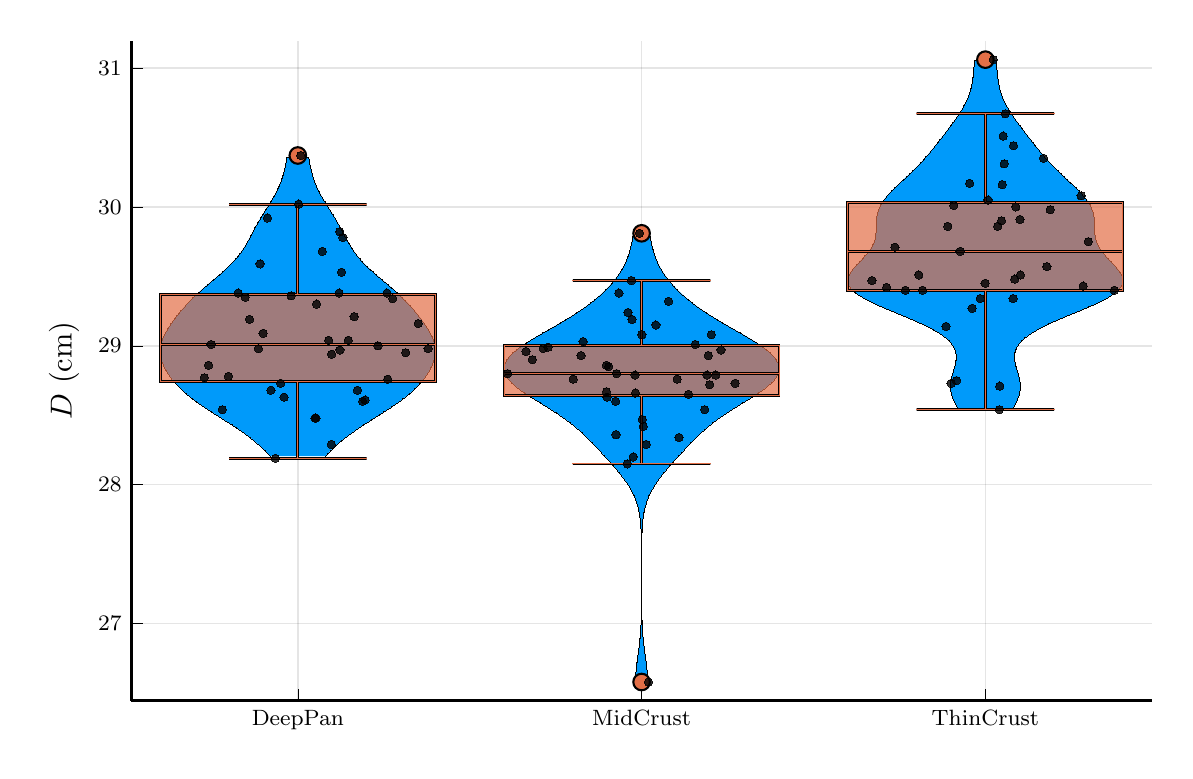
\begin{tikzpicture}[/tikz/background rectangle/.style={fill={rgb,1:red,1.0;green,1.0;blue,1.0}, draw opacity={1.0}}, show background rectangle]
\begin{axis}[point meta max={nan}, point meta min={nan}, title={}, title style={at={{(0.5,1)}}, anchor={south}, font={{\fontsize{14 pt}{18.2 pt}\selectfont}}, color={rgb,1:red,0.0;green,0.0;blue,0.0}, draw opacity={1.0}, rotate={0.0}}, legend style={color={rgb,1:red,0.0;green,0.0;blue,0.0}, draw opacity={1.0}, line width={1}, solid, fill={rgb,1:red,1.0;green,1.0;blue,1.0}, fill opacity={1.0}, text opacity={1.0}, font={{\fontsize{8 pt}{10.4 pt}\selectfont}}, text={rgb,1:red,0.0;green,0.0;blue,0.0}, cells={anchor={center}}, at={(1.02, 1)}, anchor={north west}}, axis background/.style={fill={rgb,1:red,1.0;green,1.0;blue,1.0}, opacity={1.0}}, anchor={north west}, xshift={1.0mm}, yshift={-1.0mm}, width={145.4mm}, height={99.6mm}, scaled x ticks={false}, xlabel={}, x tick style={color={rgb,1:red,0.0;green,0.0;blue,0.0}, opacity={1.0}}, x tick label style={color={rgb,1:red,0.0;green,0.0;blue,0.0}, opacity={1.0}, rotate={0}}, xlabel style={at={(ticklabel cs:0.5)}, anchor=near ticklabel, at={{(ticklabel cs:0.5)}}, anchor={near ticklabel}, font={{\fontsize{11 pt}{14.3 pt}\selectfont}}, color={rgb,1:red,0.0;green,0.0;blue,0.0}, draw opacity={1.0}, rotate={0.0}}, xmajorgrids={true}, xmin={0.01599999999999993}, xmax={2.984}, xtick={{0.5,1.5,2.5}}, xticklabels={{DeepPan,MidCrust,ThinCrust}}, xtick align={inside}, xticklabel style={font={{\fontsize{8 pt}{10.4 pt}\selectfont}}, color={rgb,1:red,0.0;green,0.0;blue,0.0}, draw opacity={1.0}, rotate={0.0}}, x grid style={color={rgb,1:red,0.0;green,0.0;blue,0.0}, draw opacity={0.1}, line width={0.5}, solid}, axis x line*={left}, x axis line style={color={rgb,1:red,0.0;green,0.0;blue,0.0}, draw opacity={1.0}, line width={1}, solid}, scaled y ticks={false}, ylabel={$D$ (cm)}, y tick style={color={rgb,1:red,0.0;green,0.0;blue,0.0}, opacity={1.0}}, y tick label style={color={rgb,1:red,0.0;green,0.0;blue,0.0}, opacity={1.0}, rotate={0}}, ylabel style={at={(ticklabel cs:0.5)}, anchor=near ticklabel, at={{(ticklabel cs:0.5)}}, anchor={near ticklabel}, font={{\fontsize{11 pt}{14.3 pt}\selectfont}}, color={rgb,1:red,0.0;green,0.0;blue,0.0}, draw opacity={1.0}, rotate={0.0}}, ymajorgrids={true}, ymin={26.4456}, ymax={31.194399999999998}, ytick={{27.0,28.0,29.0,30.0,31.0}}, yticklabels={{$27$,$28$,$29$,$30$,$31$}}, ytick align={inside}, yticklabel style={font={{\fontsize{8 pt}{10.4 pt}\selectfont}}, color={rgb,1:red,0.0;green,0.0;blue,0.0}, draw opacity={1.0}, rotate={0.0}}, y grid style={color={rgb,1:red,0.0;green,0.0;blue,0.0}, draw opacity={0.1}, line width={0.5}, solid}, axis y line*={left}, y axis line style={color={rgb,1:red,0.0;green,0.0;blue,0.0}, draw opacity={1.0}, line width={1}, solid}, colorbar={false}]
    \addplot[color={rgb,1:red,0.0;green,0.0;blue,0.0}, name path={f97bae34-bb6b-423b-aa0e-c8b635f27745}, area legend, fill={rgb,1:red,0.0;green,0.6056;blue,0.9787}, fill opacity={1.0}, draw opacity={1.0}, line width={0}, solid, forget plot]
        table[row sep={\\}]
        {
            \\
            0.5805647651104595  28.206776008421752  \\
            0.5874195409126743  28.22544077349268  \\
            0.5946620381333619  28.244105538563602  \\
            0.6023163375805013  28.26277030363453  \\
            0.6104047366150965  28.281435068705456  \\
            0.618945632012703  28.300099833776382  \\
            0.6279513109335162  28.31876459884731  \\
            0.6374258018371838  28.337429363918233  \\
            0.6473629464190047  28.35609412898916  \\
            0.6577448507086248  28.374758894060086  \\
            0.6685408578095833  28.393423659131013  \\
            0.6797071568541464  28.41208842420194  \\
            0.6911871041187776  28.430753189272863  \\
            0.7029122853444171  28.44941795434379  \\
            0.7148042963549579  28.468082719414717  \\
            0.7267771658322583  28.486747484485644  \\
            0.7387402936281958  28.505412249556567  \\
            0.7506017343028979  28.524077014627494  \\
            0.7622716223976321  28.54274177969842  \\
            0.7736655164181785  28.561406544769348  \\
            0.7847074349120176  28.580071309840275  \\
            0.7953323715966103  28.598736074911198  \\
            0.8054881072263722  28.617400839982125  \\
            0.8151361824225668  28.63606560505305  \\
            0.8242519553223646  28.65473037012398  \\
            0.8328237366389782  28.673395135194905  \\
            0.840851067485284  28.69205990026583  \\
            0.8483422762475508  28.710724665336755  \\
            0.855311513710446  28.729389430407682  \\
            0.861775514518831  28.74805419547861  \\
            0.8677503626703842  28.766718960549532  \\
            0.8732485451705458  28.78538372562046  \\
            0.8782765592253265  28.804048490691386  \\
            0.8828332946382274  28.822713255762313  \\
            0.8869093471080582  28.84137802083324  \\
            0.8904873349835141  28.860042785904163  \\
            0.8935431988720679  28.87870755097509  \\
            0.8960483689506904  28.897372316046017  \\
            0.8979725981679244  28.916037081116944  \\
            0.8992871897484948  28.934701846187867  \\
            0.8999683022123526  28.953366611258794  \\
            0.9000000000000001  28.97203137632972  \\
            0.8993767353415463  28.990696141400647  \\
            0.8981049964721136  29.009360906471574  \\
            0.8962039345454715  29.028025671542498  \\
            0.8937048794352691  29.046690436613424  \\
            0.8906497634734971  29.06535520168435  \\
            0.8870885811060291  29.084019966755278  \\
            0.8830761102701411  29.102684731826205  \\
            0.878668197835631  29.12134949689713  \\
            0.8739179586296193  29.140014261968055  \\
            0.8688722503248355  29.158679027038982  \\
            0.8635687633261775  29.17734379210991  \\
            0.8580340079966735  29.196008557180832  \\
            0.852282396871021  29.21467332225176  \\
            0.8463165155207897  29.233338087322686  \\
            0.8401285629826493  29.252002852393613  \\
            0.8337028324334075  29.27066761746454  \\
            0.8270190059492017  29.289332382535463  \\
            0.8200559630021163  29.30799714760639  \\
            0.8127957575940497  29.326661912677316  \\
            0.8052274072212591  29.345326677748243  \\
            0.797350158392027  29.36399144281917  \\
            0.7891759450500033  29.382656207890093  \\
            0.7807308319912467  29.40132097296102  \\
            0.7720553270973143  29.419985738031947  \\
            0.763203544664901  29.438650503102874  \\
            0.7542412978692841  29.457315268173797  \\
            0.7452432828535553  29.475980033244724  \\
            0.7362895831364028  29.49464479831565  \\
            0.7274617662641327  29.513309563386578  \\
            0.7188388627265583  29.531974328457505  \\
            0.7104935104898816  29.550639093528428  \\
            0.7024885197341597  29.569303858599355  \\
            0.6948740659764072  29.58796862367028  \\
            0.6876856613382545  29.60663338874121  \\
            0.6809429893856268  29.625298153812135  \\
            0.6746496246548601  29.64396291888306  \\
            0.6687935988733051  29.662627683953986  \\
            0.6633487260206731  29.681292449024912  \\
            0.6582765604137788  29.69995721409584  \\
            0.6535288371467469  29.718621979166763  \\
            0.6490502323625674  29.73728674423769  \\
            0.6447812807481452  29.755951509308616  \\
            0.6406612973179074  29.774616274379543  \\
            0.6366311675133393  29.79328103945047  \\
            0.6326358913102299  29.811945804521393  \\
            0.6286267909704067  29.83061056959232  \\
            0.6245633162604871  29.849275334663247  \\
            0.6204144038624291  29.867940099734174  \\
            0.6161593683608851  29.886604864805097  \\
            0.6117883201921511  29.905269629876024  \\
            0.6073021213135666  29.92393439494695  \\
            0.6027119024584441  29.942599160017878  \\
            0.5980381772090988  29.961263925088804  \\
            0.5933095982958028  29.979928690159728  \\
            0.5885614109394303  29.998593455230655  \\
            0.5838336669031023  30.01725822030158  \\
            0.5791692711213074  30.03592298537251  \\
            0.5746119399561161  30.054587750443435  \\
            0.5702041556555476  30.07325251551436  \\
            0.5659852046544277  30.091917280585285  \\
            0.5619893871079916  30.110582045656212  \\
            0.5582444807170939  30.12924681072714  \\
            0.5547705329561979  30.147911575798062  \\
            0.5515790420716598  30.16657634086899  \\
            0.5486725689429026  30.185241105939916  \\
            0.5460447998414496  30.203905871010843  \\
            0.5436810554959451  30.22257063608177  \\
            0.5415592162748292  30.241235401152693  \\
            0.5396510085851411  30.25990016622362  \\
            0.5379235756887198  30.278564931294547  \\
            0.5363412388734863  30.297229696365473  \\
            0.5348673437964194  30.3158944614364  \\
            0.5334660828675037  30.334559226507324  \\
            0.5321041882009158  30.35322399157825  \\
            0.4678958117990843  30.35322399157825  \\
            0.4665339171324962  30.334559226507324  \\
            0.46513265620358063  30.3158944614364  \\
            0.4636587611265138  30.297229696365473  \\
            0.4620764243112802  30.278564931294547  \\
            0.4603489914148589  30.25990016622362  \\
            0.45844078372517083  30.241235401152693  \\
            0.45631894450405486  30.22257063608177  \\
            0.4539552001585504  30.203905871010843  \\
            0.4513274310570974  30.185241105939916  \\
            0.44842095792834025  30.16657634086899  \\
            0.4452294670438021  30.147911575798062  \\
            0.44175551928290613  30.12924681072714  \\
            0.4380106128920083  30.110582045656212  \\
            0.4340147953455723  30.091917280585285  \\
            0.4297958443444524  30.07325251551436  \\
            0.4253880600438839  30.054587750443435  \\
            0.42083072887869255  30.03592298537251  \\
            0.4161663330968977  30.01725822030158  \\
            0.4114385890605697  29.998593455230655  \\
            0.40669040170419724  29.979928690159728  \\
            0.40196182279090115  29.961263925088804  \\
            0.3972880975415559  29.942599160017878  \\
            0.39269787868643335  29.92393439494695  \\
            0.3882116798078489  29.905269629876024  \\
            0.38384063163911486  29.886604864805097  \\
            0.37958559613757087  29.867940099734174  \\
            0.3754366837395129  29.849275334663247  \\
            0.37137320902959325  29.83061056959232  \\
            0.36736410868977015  29.811945804521393  \\
            0.36336883248666074  29.79328103945047  \\
            0.35933870268209256  29.774616274379543  \\
            0.3552187192518548  29.755951509308616  \\
            0.3509497676374326  29.73728674423769  \\
            0.3464711628532531  29.718621979166763  \\
            0.34172343958622126  29.69995721409584  \\
            0.3366512739793269  29.681292449024912  \\
            0.3312064011266948  29.662627683953986  \\
            0.3253503753451399  29.64396291888306  \\
            0.3190570106143732  29.625298153812135  \\
            0.31231433866174557  29.60663338874121  \\
            0.30512593402359284  29.58796862367028  \\
            0.2975114802658403  29.569303858599355  \\
            0.28950648951011837  29.550639093528428  \\
            0.2811611372734418  29.531974328457505  \\
            0.2725382337358673  29.513309563386578  \\
            0.2637104168635972  29.49464479831565  \\
            0.25475671714644466  29.475980033244724  \\
            0.245758702130716  29.457315268173797  \\
            0.23679645533509897  29.438650503102874  \\
            0.22794467290268572  29.419985738031947  \\
            0.21926916800875323  29.40132097296102  \\
            0.21082405494999673  29.382656207890093  \\
            0.202649841607973  29.36399144281917  \\
            0.19477259277874093  29.345326677748243  \\
            0.1872042424059503  29.326661912677316  \\
            0.1799440369978837  29.30799714760639  \\
            0.1729809940507983  29.289332382535463  \\
            0.16629716756659252  29.27066761746454  \\
            0.15987143701735074  29.252002852393613  \\
            0.15368348447921032  29.233338087322686  \\
            0.14771760312897897  29.21467332225176  \\
            0.14196599200332655  29.196008557180832  \\
            0.13643123667382245  29.17734379210991  \\
            0.1311277496751645  29.158679027038982  \\
            0.12608204137038076  29.140014261968055  \\
            0.12133180216436906  29.12134949689713  \\
            0.1169238897298589  29.102684731826205  \\
            0.11291141889397094  29.084019966755278  \\
            0.10935023652650289  29.06535520168435  \\
            0.10629512056473095  29.046690436613424  \\
            0.10379606545452852  29.028025671542498  \\
            0.10189500352788639  29.009360906471574  \\
            0.10062326465845367  28.990696141400647  \\
            0.09999999999999992  28.97203137632972  \\
            0.10003169778764748  28.953366611258794  \\
            0.10071281025150525  28.934701846187867  \\
            0.10202740183207559  28.916037081116944  \\
            0.10395163104930966  28.897372316046017  \\
            0.10645680112793204  28.87870755097509  \\
            0.10951266501648593  28.860042785904163  \\
            0.11309065289194176  28.84137802083324  \\
            0.1171667053617727  28.822713255762313  \\
            0.12172344077467351  28.804048490691386  \\
            0.1267514548294542  28.78538372562046  \\
            0.1322496373296158  28.766718960549532  \\
            0.13822448548116895  28.74805419547861  \\
            0.144688486289554  28.729389430407682  \\
            0.1516577237524493  28.710724665336755  \\
            0.1591489325147159  28.69205990026583  \\
            0.16717626336102176  28.673395135194905  \\
            0.17574804467763538  28.65473037012398  \\
            0.1848638175774332  28.63606560505305  \\
            0.1945118927736278  28.617400839982125  \\
            0.2046676284033897  28.598736074911198  \\
            0.21529256508798245  28.580071309840275  \\
            0.22633448358182157  28.561406544769348  \\
            0.23772837760236787  28.54274177969842  \\
            0.2493982656971021  28.524077014627494  \\
            0.2612597063718042  28.505412249556567  \\
            0.27322283416774173  28.486747484485644  \\
            0.28519570364504204  28.468082719414717  \\
            0.2970877146555829  28.44941795434379  \\
            0.3088128958812224  28.430753189272863  \\
            0.32029284314585355  28.41208842420194  \\
            0.3314591421904168  28.393423659131013  \\
            0.3422551492913753  28.374758894060086  \\
            0.35263705358099534  28.35609412898916  \\
            0.3625741981628162  28.337429363918233  \\
            0.3720486890664838  28.31876459884731  \\
            0.38105436798729697  28.300099833776382  \\
            0.38959526338490347  28.281435068705456  \\
            0.3976836624194987  28.26277030363453  \\
            0.4053379618666381  28.244105538563602  \\
            0.4125804590873256  28.22544077349268  \\
            0.4194352348895405  28.206776008421752  \\
        }
        ;
    \addplot[color={rgb,1:red,0.0;green,0.0;blue,0.0}, name path={f97bae34-bb6b-423b-aa0e-c8b635f27745}, area legend, fill={rgb,1:red,0.0;green,0.6056;blue,0.9787}, fill opacity={1.0}, draw opacity={1.0}, line width={0}, solid, forget plot]
        table[row sep={\\}]
        {
            \\
            1.5175553478731572  26.60291372579849  \\
            1.5171613996778615  26.626854872778964  \\
            1.51651705861397  26.650796019759436  \\
            1.5156512675445943  26.67473716673991  \\
            1.514601692094512  26.698678313720386  \\
            1.5134120074959487  26.72261946070086  \\
            1.5121288991469974  26.74656060768133  \\
            1.5107990622592902  26.770501754661804  \\
            1.5094664650389247  26.79444290164228  \\
            1.5081700896892087  26.818384048622754  \\
            1.5069422952614233  26.842325195603227  \\
            1.5058078671658757  26.8662663425837  \\
            1.504783741218633  26.890207489564176  \\
            1.5038793249751659  26.91414863654465  \\
            1.5030972923693646  26.938089783525122  \\
            1.5024347023616138  26.9620309305056  \\
            1.5018842879641692  26.98597207748607  \\
            1.5014357754002083  27.009913224466544  \\
            1.5010771191911763  27.033854371447017  \\
            1.5007955718748245  27.057795518427493  \\
            1.5005785413504007  27.081736665407966  \\
            1.5004142200870396  27.10567781238844  \\
            1.5002919956306835  27.129618959368912  \\
            1.5002026695582154  27.15356010634939  \\
            1.5001385221716648  27.17750125332986  \\
            1.5000932637352762  27.201442400310334  \\
            1.500061911477972  27.225383547290807  \\
            1.5000406266790518  27.249324694271284  \\
            1.5000265396044838  27.273265841251757  \\
            1.5000175832533658  27.29720698823223  \\
            1.5000123508086174  27.321148135212702  \\
            1.5000099869598948  27.34508928219318  \\
            1.5000101201172145  27.36903042917365  \\
            1.5000128409077198  27.392971576154125  \\
            1.5000187319747984  27.4169127231346  \\
            1.5000289545519878  27.440853870115074  \\
            1.5000453980273707  27.464795017095547  \\
            1.5000708991343656  27.48873616407602  \\
            1.5001095368433983  27.512677311056496  \\
            1.5001670068235575  27.53661845803697  \\
            1.5002510748918136  27.560559605017442  \\
            1.5003721017210347  27.584500751997915  \\
            1.5005436210628844  27.60844189897839  \\
            1.5007829410950007  27.632383045958864  \\
            1.5011117239997807  27.656324192939337  \\
            1.5015564839238553  27.68026533991981  \\
            1.5021489300765785  27.704206486900286  \\
            1.5029260724338214  27.72814763388076  \\
            1.5039300051022086  27.752088780861232  \\
            1.505207289509352  27.776029927841705  \\
            1.506807878225419  27.79997107482218  \\
            1.508783551245895  27.823912221802654  \\
            1.511185879227885  27.847853368783127  \\
            1.5140637798514762  27.8717945157636  \\
            1.5174607896765557  27.895735662744077  \\
            1.5214122285347749  27.91967680972455  \\
            1.5259424796750922  27.943617956705022  \\
            1.5310626395779412  27.9675591036855  \\
            1.5367688005291464  27.991500250665972  \\
            1.5430412125302027  28.015441397646445  \\
            1.5498445272953234  28.039382544626918  \\
            1.5571292572024318  28.063323691607394  \\
            1.5648344901890727  28.087264838587867  \\
            1.5728917941771254  28.11120598556834  \\
            1.581230129897468  28.135147132548813  \\
            1.5897814782500281  28.15908827952929  \\
            1.5984867872709474  28.183029426509762  \\
            1.607301763973925  28.206970573490235  \\
            1.6162019868428972  28.230911720470708  \\
            1.6251868036681174  28.254852867451184  \\
            1.634281513275134  28.278794014431657  \\
            1.6435374126364808  28.30273516141213  \\
            1.6530294235184086  28.326676308392603  \\
            1.662851191124311  28.35061745537308  \\
            1.6731077613342475  28.374558602353552  \\
            1.6839061770883916  28.398499749334025  \\
            1.695344566495264  28.422440896314498  \\
            1.7075004996134324  28.446382043294975  \\
            1.720419540670229  28.470323190275447  \\
            1.734104993518584  28.49426433725592  \\
            1.74850981297785  28.518205484236397  \\
            1.763531526476078  28.54214663121687  \\
            1.779010785260232  28.566087778197343  \\
            1.7947338621415958  28.590028925177815  \\
            1.81043906501356  28.613970072158292  \\
            1.825826681979505  28.637911219138765  \\
            1.8405717570578664  28.661852366119238  \\
            1.8543387533147864  28.68579351309971  \\
            1.8667970210936695  28.709734660080187  \\
            1.8776359663325968  28.73367580706066  \\
            1.8865789045987165  28.757616954041133  \\
            1.8933947712708707  28.781558101021606  \\
            1.8979071057830263  28.805499248002082  \\
            1.9  28.829440394982555  \\
            1.8996209599749596  28.853381541963028  \\
            1.8967808457466266  28.8773226889435  \\
            1.8915512064278153  28.901263835923977  \\
            1.8840594125702368  28.92520498290445  \\
            1.8744820128715831  28.949146129884923  \\
            1.8630367257229419  28.973087276865396  \\
            1.849973440394483  28.997028423845872  \\
            1.8355645690294113  29.020969570826345  \\
            1.8200950739327975  29.044910717806818  \\
            1.803852500334312  29.068851864787295  \\
            1.7871173682617765  29.092793011767768  \\
            1.770154305619513  29.11673415874824  \\
            1.7532043208672952  29.140675305728713  \\
            1.7364786009495499  29.16461645270919  \\
            1.7201541661046347  29.188557599689663  \\
            1.7043716135150442  29.212498746670136  \\
            1.6892350412645727  29.23643989365061  \\
            1.6748140761340773  29.260381040631085  \\
            1.6611477530150245  29.284322187611558  \\
            1.6482498325930992  29.30826333459203  \\
            1.636115018963598  29.332204481572504  \\
            1.6247254671689197  29.35614562855298  \\
            1.614056962640662  29.380086775533453  \\
            1.604084212351627  29.404027922513926  \\
            1.594784805007297  29.4279690694944  \\
            1.5861415613747658  29.451910216474875  \\
            1.5781431868851796  29.475851363455348  \\
            1.5707833348276106  29.49979251043582  \\
            1.5640583671365484  29.523733657416297  \\
            1.5579642404427225  29.54767480439677  \\
            1.5524930317047707  29.571615951377243  \\
            1.5476296407963581  29.595557098357716  \\
            1.5433491649747426  29.619498245338193  \\
            1.5396153382968263  29.643439392318665  \\
            1.536380281256143  29.66738053929914  \\
            1.5335856314492426  29.69132168627961  \\
            1.5311649475426365  29.715262833260088  \\
            1.529047119146433  29.73920398024056  \\
            1.5271603945560954  29.763145127221033  \\
            1.5254365712369904  29.787086274201506  \\
            1.4745634287630096  29.787086274201506  \\
            1.4728396054439046  29.763145127221033  \\
            1.470952880853567  29.73920398024056  \\
            1.4688350524573635  29.715262833260088  \\
            1.4664143685507574  29.69132168627961  \\
            1.463619718743857  29.66738053929914  \\
            1.4603846617031737  29.643439392318665  \\
            1.4566508350252574  29.619498245338193  \\
            1.4523703592036419  29.595557098357716  \\
            1.4475069682952293  29.571615951377243  \\
            1.4420357595572775  29.54767480439677  \\
            1.4359416328634516  29.523733657416297  \\
            1.4292166651723894  29.49979251043582  \\
            1.4218568131148204  29.475851363455348  \\
            1.4138584386252342  29.451910216474875  \\
            1.405215194992703  29.4279690694944  \\
            1.395915787648373  29.404027922513926  \\
            1.385943037359338  29.380086775533453  \\
            1.3752745328310803  29.35614562855298  \\
            1.363884981036402  29.332204481572504  \\
            1.3517501674069008  29.30826333459203  \\
            1.3388522469849755  29.284322187611558  \\
            1.3251859238659227  29.260381040631085  \\
            1.3107649587354273  29.23643989365061  \\
            1.2956283864849558  29.212498746670136  \\
            1.2798458338953653  29.188557599689663  \\
            1.2635213990504501  29.16461645270919  \\
            1.2467956791327048  29.140675305728713  \\
            1.229845694380487  29.11673415874824  \\
            1.2128826317382235  29.092793011767768  \\
            1.196147499665688  29.068851864787295  \\
            1.1799049260672025  29.044910717806818  \\
            1.1644354309705887  29.020969570826345  \\
            1.150026559605517  28.997028423845872  \\
            1.1369632742770581  28.973087276865396  \\
            1.1255179871284169  28.949146129884923  \\
            1.1159405874297632  28.92520498290445  \\
            1.1084487935721847  28.901263835923977  \\
            1.1032191542533734  28.8773226889435  \\
            1.1003790400250404  28.853381541963028  \\
            1.1  28.829440394982555  \\
            1.1020928942169737  28.805499248002082  \\
            1.1066052287291293  28.781558101021606  \\
            1.1134210954012835  28.757616954041133  \\
            1.1223640336674032  28.73367580706066  \\
            1.1332029789063305  28.709734660080187  \\
            1.1456612466852136  28.68579351309971  \\
            1.1594282429421336  28.661852366119238  \\
            1.174173318020495  28.637911219138765  \\
            1.18956093498644  28.613970072158292  \\
            1.2052661378584042  28.590028925177815  \\
            1.220989214739768  28.566087778197343  \\
            1.236468473523922  28.54214663121687  \\
            1.25149018702215  28.518205484236397  \\
            1.265895006481416  28.49426433725592  \\
            1.279580459329771  28.470323190275447  \\
            1.2924995003865676  28.446382043294975  \\
            1.304655433504736  28.422440896314498  \\
            1.3160938229116084  28.398499749334025  \\
            1.3268922386657525  28.374558602353552  \\
            1.337148808875689  28.35061745537308  \\
            1.3469705764815914  28.326676308392603  \\
            1.3564625873635192  28.30273516141213  \\
            1.365718486724866  28.278794014431657  \\
            1.3748131963318826  28.254852867451184  \\
            1.3837980131571028  28.230911720470708  \\
            1.392698236026075  28.206970573490235  \\
            1.4015132127290526  28.183029426509762  \\
            1.4102185217499719  28.15908827952929  \\
            1.418769870102532  28.135147132548813  \\
            1.4271082058228746  28.11120598556834  \\
            1.4351655098109273  28.087264838587867  \\
            1.4428707427975682  28.063323691607394  \\
            1.4501554727046766  28.039382544626918  \\
            1.4569587874697973  28.015441397646445  \\
            1.4632311994708536  27.991500250665972  \\
            1.4689373604220588  27.9675591036855  \\
            1.4740575203249078  27.943617956705022  \\
            1.4785877714652251  27.91967680972455  \\
            1.4825392103234443  27.895735662744077  \\
            1.4859362201485238  27.8717945157636  \\
            1.488814120772115  27.847853368783127  \\
            1.491216448754105  27.823912221802654  \\
            1.493192121774581  27.79997107482218  \\
            1.494792710490648  27.776029927841705  \\
            1.4960699948977914  27.752088780861232  \\
            1.4970739275661786  27.72814763388076  \\
            1.4978510699234215  27.704206486900286  \\
            1.4984435160761447  27.68026533991981  \\
            1.4988882760002193  27.656324192939337  \\
            1.4992170589049993  27.632383045958864  \\
            1.4994563789371156  27.60844189897839  \\
            1.4996278982789653  27.584500751997915  \\
            1.4997489251081864  27.560559605017442  \\
            1.4998329931764425  27.53661845803697  \\
            1.4998904631566017  27.512677311056496  \\
            1.4999291008656344  27.48873616407602  \\
            1.4999546019726293  27.464795017095547  \\
            1.4999710454480122  27.440853870115074  \\
            1.4999812680252016  27.4169127231346  \\
            1.4999871590922802  27.392971576154125  \\
            1.4999898798827855  27.36903042917365  \\
            1.4999900130401052  27.34508928219318  \\
            1.4999876491913826  27.321148135212702  \\
            1.4999824167466342  27.29720698823223  \\
            1.4999734603955162  27.273265841251757  \\
            1.4999593733209482  27.249324694271284  \\
            1.499938088522028  27.225383547290807  \\
            1.4999067362647238  27.201442400310334  \\
            1.4998614778283352  27.17750125332986  \\
            1.4997973304417846  27.15356010634939  \\
            1.4997080043693165  27.129618959368912  \\
            1.4995857799129604  27.10567781238844  \\
            1.4994214586495993  27.081736665407966  \\
            1.4992044281251755  27.057795518427493  \\
            1.4989228808088237  27.033854371447017  \\
            1.4985642245997917  27.009913224466544  \\
            1.4981157120358308  26.98597207748607  \\
            1.4975652976383862  26.9620309305056  \\
            1.4969027076306354  26.938089783525122  \\
            1.4961206750248341  26.91414863654465  \\
            1.495216258781367  26.890207489564176  \\
            1.4941921328341243  26.8662663425837  \\
            1.4930577047385767  26.842325195603227  \\
            1.4918299103107913  26.818384048622754  \\
            1.4905335349610753  26.79444290164228  \\
            1.4892009377407098  26.770501754661804  \\
            1.4878711008530026  26.74656060768133  \\
            1.4865879925040513  26.72261946070086  \\
            1.485398307905488  26.698678313720386  \\
            1.4843487324554057  26.67473716673991  \\
            1.48348294138603  26.650796019759436  \\
            1.4828386003221385  26.626854872778964  \\
            1.4824446521268428  26.60291372579849  \\
        }
        ;
    \addplot[color={rgb,1:red,0.0;green,0.0;blue,0.0}, name path={f97bae34-bb6b-423b-aa0e-c8b635f27745}, area legend, fill={rgb,1:red,0.0;green,0.6056;blue,0.9787}, fill opacity={1.0}, draw opacity={1.0}, line width={0}, solid, forget plot]
        table[row sep={\\}]
        {
            \\
            2.5786188831628643  28.547041571253622  \\
            2.583591995366583  28.567414879038118  \\
            2.588127510942612  28.58778818682261  \\
            2.5921243173018587  28.608161494607106  \\
            2.5954929475067625  28.6285348023916  \\
            2.598160611164346  28.64890811017609  \\
            2.600075962598895  28.669281417960587  \\
            2.6012133135027264  28.68965472574508  \\
            2.601576009438931  28.710028033529575  \\
            2.6011987262399248  28.730401341314067  \\
            2.6001485017987758  28.750774649098563  \\
            2.5985243963707414  28.771147956883055  \\
            2.596455763128194  28.79152126466755  \\
            2.594099201406682  28.811894572452044  \\
            2.5916343482326325  28.83226788023654  \\
            2.5892587303309376  28.852641188021032  \\
            2.5871819417558903  28.873014495805524  \\
            2.5856194274186564  28.89338780359002  \\
            2.5847861396142973  28.913761111374512  \\
            2.5848902965706384  28.934134419159008  \\
            2.5861274159634804  28.9545077269435  \\
            2.588674731827453  28.974881034727996  \\
            2.5926860412424144  28.99525434251249  \\
            2.5982869782792783  29.015627650296985  \\
            2.60557068581326  29.036000958081477  \\
            2.614593856575333  29.05637426586597  \\
            2.625373144543736  29.076747573650465  \\
            2.637882003026829  29.097120881434957  \\
            2.6520480784868363  29.117494189219453  \\
            2.667751367437035  29.137867497003946  \\
            2.684823413376435  29.15824080478844  \\
            2.703047866961353  29.178614112572934  \\
            2.7221627422831896  29.19898742035743  \\
            2.741864665667242  29.219360728141922  \\
            2.7618153265849132  29.239734035926418  \\
            2.7816502052697314  29.26010734371091  \\
            2.8009894773979322  29.280480651495402  \\
            2.8194507978925873  29.300853959279898  \\
            2.8366634634583026  29.32122726706439  \\
            2.8522832693592846  29.341600574848886  \\
            2.8660072326387964  29.36197388263338  \\
            2.877587270950854  29.382347190417875  \\
            2.8868419174265187  29.402720498202367  \\
            2.8936652239897995  29.423093805986863  \\
            2.8980321560852915  29.443467113771355  \\
            2.9  29.46384042155585  \\
            2.899705571342389  29.484213729340343  \\
            2.897358305684698  29.504587037124836  \\
            2.8932296029576117  29.52496034490933  \\
            2.8876390592636434  29.545333652693824  \\
            2.8809384299968346  29.56570696047832  \\
            2.8734943089996485  29.586080268262812  \\
            2.8656705699815084  29.606453576047308  \\
            2.857811596859203  29.6268268838318  \\
            2.850227235276391  29.647200191616296  \\
            2.84318024118924  29.66757349940079  \\
            2.836876801620421  29.687946807185284  \\
            2.8314604773752405  29.708320114969776  \\
            2.8270096875472257  29.72869342275427  \\
            2.823538638793282  29.749066730538765  \\
            2.821001412797171  29.769440038323257  \\
            2.8192987727722065  29.789813346107753  \\
            2.818287139366422  29.810186653892245  \\
            2.81778911882419  29.83055996167674  \\
            2.817604939292199  29.850933269461233  \\
            2.8175241600363194  29.87130657724573  \\
            2.8173370571736056  29.89167988503022  \\
            2.816845152161267  29.912053192814714  \\
            2.8158704299284016  29.93242650059921  \\
            2.8142628870844093  29.952799808383702  \\
            2.8119061527164555  29.973173116168198  \\
            2.8087210310746  29.99354642395269  \\
            2.8046669233800317  30.013919731737186  \\
            2.7997411914989563  30.03429303952168  \\
            2.7939766255026552  30.054666347306174  \\
            2.787437266119987  30.075039655090666  \\
            2.7802129075883046  30.095412962875162  \\
            2.772412662390653  30.115786270659655  \\
            2.7641580033687587  30.136159578444147  \\
            2.75557570828109  30.156532886228643  \\
            2.746791116029642  30.176906194013135  \\
            2.7379220632512373  30.19727950179763  \\
            2.7290738073871665  30.217652809582123  \\
            2.7203351621533707  30.23802611736662  \\
            2.7117759795070127  30.25839942515111  \\
            2.70344601576763  30.278772732935607  \\
            2.69537512594302  30.2991460407201  \\
            2.687574646680438  30.319519348504596  \\
            2.680039760763787  30.339892656289088  \\
            2.6727525892460955  30.36026596407358  \\
            2.665685733623896  30.380639271858076  \\
            2.6588059901292764  30.40101257964257  \\
            2.6520779792034195  30.421385887427064  \\
            2.645467471552135  30.441759195211556  \\
            2.6389442424832  30.462132502996052  \\
            2.6324843423642763  30.482505810780545  \\
            2.626071726906961  30.50287911856504  \\
            2.6196992411966438  30.523252426349533  \\
            2.613368991897348  30.54362573413403  \\
            2.6070921705386083  30.56399904191852  \\
            2.600888406782056  30.584372349703013  \\
            2.594784735366043  30.60474565748751  \\
            2.588814256729189  30.625118965272  \\
            2.583014562663687  30.645492273056497  \\
            2.5774259885069224  30.66586558084099  \\
            2.572089745681611  30.686238888625486  \\
            2.5670459852082175  30.706612196409978  \\
            2.5623318451711175  30.726985504194474  \\
            2.55797954257866  30.747358811978966  \\
            2.5540145808049433  30.76773211976346  \\
            2.550454154988922  30.788105427547954  \\
            2.547305846012287  30.808478735332447  \\
            2.5445666956619135  30.828852043116942  \\
            2.5422227486435336  30.849225350901435  \\
            2.54024912974935  30.86959865868593  \\
            2.5386106966854434  30.889971966470423  \\
            2.5372632724318973  30.91034527425492  \\
            2.536155418611942  30.93071858203941  \\
            2.535230667380872  30.951091889823907  \\
            2.5344300886005033  30.9714651976084  \\
            2.533695036296165  30.99183850539289  \\
            2.532969897683761  31.012211813177387  \\
            2.5322046622545438  31.03258512096188  \\
            2.5313571387315434  31.052958428746376  \\
            2.4686428612684566  31.052958428746376  \\
            2.4677953377454562  31.03258512096188  \\
            2.467030102316239  31.012211813177387  \\
            2.466304963703835  30.99183850539289  \\
            2.4655699113994967  30.9714651976084  \\
            2.464769332619128  30.951091889823907  \\
            2.463844581388058  30.93071858203941  \\
            2.4627367275681027  30.91034527425492  \\
            2.4613893033145566  30.889971966470423  \\
            2.45975087025065  30.86959865868593  \\
            2.4577772513564664  30.849225350901435  \\
            2.4554333043380865  30.828852043116942  \\
            2.452694153987713  30.808478735332447  \\
            2.449545845011078  30.788105427547954  \\
            2.4459854191950567  30.76773211976346  \\
            2.44202045742134  30.747358811978966  \\
            2.4376681548288825  30.726985504194474  \\
            2.4329540147917825  30.706612196409978  \\
            2.427910254318389  30.686238888625486  \\
            2.4225740114930776  30.66586558084099  \\
            2.416985437336313  30.645492273056497  \\
            2.411185743270811  30.625118965272  \\
            2.405215264633957  30.60474565748751  \\
            2.399111593217944  30.584372349703013  \\
            2.3929078294613917  30.56399904191852  \\
            2.386631008102652  30.54362573413403  \\
            2.3803007588033562  30.523252426349533  \\
            2.373928273093039  30.50287911856504  \\
            2.3675156576357237  30.482505810780545  \\
            2.3610557575168  30.462132502996052  \\
            2.354532528447865  30.441759195211556  \\
            2.3479220207965805  30.421385887427064  \\
            2.3411940098707236  30.40101257964257  \\
            2.334314266376104  30.380639271858076  \\
            2.3272474107539045  30.36026596407358  \\
            2.319960239236213  30.339892656289088  \\
            2.312425353319562  30.319519348504596  \\
            2.30462487405698  30.2991460407201  \\
            2.29655398423237  30.278772732935607  \\
            2.2882240204929873  30.25839942515111  \\
            2.2796648378466293  30.23802611736662  \\
            2.2709261926128335  30.217652809582123  \\
            2.2620779367487627  30.19727950179763  \\
            2.253208883970358  30.176906194013135  \\
            2.24442429171891  30.156532886228643  \\
            2.2358419966312413  30.136159578444147  \\
            2.227587337609347  30.115786270659655  \\
            2.2197870924116954  30.095412962875162  \\
            2.212562733880013  30.075039655090666  \\
            2.2060233744973448  30.054666347306174  \\
            2.2002588085010437  30.03429303952168  \\
            2.1953330766199683  30.013919731737186  \\
            2.1912789689254  29.99354642395269  \\
            2.1880938472835445  29.973173116168198  \\
            2.1857371129155907  29.952799808383702  \\
            2.1841295700715984  29.93242650059921  \\
            2.183154847838733  29.912053192814714  \\
            2.1826629428263944  29.89167988503022  \\
            2.1824758399636806  29.87130657724573  \\
            2.182395060707801  29.850933269461233  \\
            2.18221088117581  29.83055996167674  \\
            2.181712860633578  29.810186653892245  \\
            2.1807012272277935  29.789813346107753  \\
            2.178998587202829  29.769440038323257  \\
            2.176461361206718  29.749066730538765  \\
            2.1729903124527743  29.72869342275427  \\
            2.1685395226247595  29.708320114969776  \\
            2.163123198379579  29.687946807185284  \\
            2.15681975881076  29.66757349940079  \\
            2.149772764723609  29.647200191616296  \\
            2.142188403140797  29.6268268838318  \\
            2.1343294300184916  29.606453576047308  \\
            2.1265056910003515  29.586080268262812  \\
            2.1190615700031654  29.56570696047832  \\
            2.1123609407363566  29.545333652693824  \\
            2.1067703970423883  29.52496034490933  \\
            2.102641694315302  29.504587037124836  \\
            2.100294428657611  29.484213729340343  \\
            2.1  29.46384042155585  \\
            2.1019678439147085  29.443467113771355  \\
            2.1063347760102005  29.423093805986863  \\
            2.1131580825734813  29.402720498202367  \\
            2.122412729049146  29.382347190417875  \\
            2.1339927673612036  29.36197388263338  \\
            2.1477167306407154  29.341600574848886  \\
            2.1633365365416974  29.32122726706439  \\
            2.1805492021074127  29.300853959279898  \\
            2.1990105226020678  29.280480651495402  \\
            2.2183497947302686  29.26010734371091  \\
            2.2381846734150868  29.239734035926418  \\
            2.258135334332758  29.219360728141922  \\
            2.2778372577168104  29.19898742035743  \\
            2.296952133038647  29.178614112572934  \\
            2.315176586623565  29.15824080478844  \\
            2.332248632562965  29.137867497003946  \\
            2.3479519215131637  29.117494189219453  \\
            2.362117996973171  29.097120881434957  \\
            2.374626855456264  29.076747573650465  \\
            2.385406143424667  29.05637426586597  \\
            2.39442931418674  29.036000958081477  \\
            2.4017130217207217  29.015627650296985  \\
            2.4073139587575856  28.99525434251249  \\
            2.411325268172547  28.974881034727996  \\
            2.4138725840365196  28.9545077269435  \\
            2.4151097034293616  28.934134419159008  \\
            2.4152138603857027  28.913761111374512  \\
            2.4143805725813436  28.89338780359002  \\
            2.4128180582441097  28.873014495805524  \\
            2.4107412696690624  28.852641188021032  \\
            2.4083656517673675  28.83226788023654  \\
            2.405900798593318  28.811894572452044  \\
            2.403544236871806  28.79152126466755  \\
            2.4014756036292586  28.771147956883055  \\
            2.3998514982012242  28.750774649098563  \\
            2.3988012737600752  28.730401341314067  \\
            2.398423990561069  28.710028033529575  \\
            2.3987866864972736  28.68965472574508  \\
            2.399924037401105  28.669281417960587  \\
            2.401839388835654  28.64890811017609  \\
            2.4045070524932375  28.6285348023916  \\
            2.4078756826981413  28.608161494607106  \\
            2.411872489057388  28.58778818682261  \\
            2.416408004633417  28.567414879038118  \\
            2.4213811168371357  28.547041571253622  \\
        }
        ;
    \addplot[color={rgb,1:red,0.0;green,0.0;blue,0.0}, name path={09ca2b63-05bd-4c17-a186-0003500b0333}, area legend, fill={rgb,1:red,0.8889;green,0.4356;blue,0.2781}, fill opacity={0.7}, draw opacity={1.0}, line width={1}, solid, forget plot]
        table[row sep={\\}]
        {
            \\
            0.5  28.19  \\
            0.3  28.19  \\
            0.7  28.19  \\
            0.5  28.19  \\
            0.5  28.745  \\
        }
        ;
    \addplot[color={rgb,1:red,0.0;green,0.0;blue,0.0}, name path={09ca2b63-05bd-4c17-a186-0003500b0333}, area legend, fill={rgb,1:red,0.8889;green,0.4356;blue,0.2781}, fill opacity={0.7}, draw opacity={1.0}, line width={1}, solid, forget plot]
        table[row sep={\\}]
        {
            \\
            0.9  28.745  \\
            0.9  29.01  \\
            0.09999999999999998  29.01  \\
            0.09999999999999998  28.745  \\
            0.9  28.745  \\
            0.9  29.01  \\
        }
        ;
    \addplot[color={rgb,1:red,0.0;green,0.0;blue,0.0}, name path={09ca2b63-05bd-4c17-a186-0003500b0333}, area legend, fill={rgb,1:red,0.8889;green,0.4356;blue,0.2781}, fill opacity={0.7}, draw opacity={1.0}, line width={1}, solid, forget plot]
        table[row sep={\\}]
        {
            \\
            0.9  29.369999999999997  \\
            0.09999999999999998  29.369999999999997  \\
            0.09999999999999998  29.01  \\
            0.9  29.01  \\
            0.9  29.369999999999997  \\
            0.5  29.369999999999997  \\
        }
        ;
    \addplot[color={rgb,1:red,0.0;green,0.0;blue,0.0}, name path={09ca2b63-05bd-4c17-a186-0003500b0333}, area legend, fill={rgb,1:red,0.8889;green,0.4356;blue,0.2781}, fill opacity={0.7}, draw opacity={1.0}, line width={1}, solid, forget plot]
        table[row sep={\\}]
        {
            \\
            0.5  30.02  \\
            0.3  30.02  \\
            0.7  30.02  \\
            0.5  30.02  \\
            0.5  29.369999999999997  \\
        }
        ;
    \addplot[color={rgb,1:red,0.0;green,0.0;blue,0.0}, name path={09ca2b63-05bd-4c17-a186-0003500b0333}, area legend, fill={rgb,1:red,0.8889;green,0.4356;blue,0.2781}, fill opacity={0.7}, draw opacity={1.0}, line width={1}, solid, forget plot]
        table[row sep={\\}]
        {
            \\
            1.5  28.15  \\
            1.3  28.15  \\
            1.7  28.15  \\
            1.5  28.15  \\
            1.5  28.64  \\
        }
        ;
    \addplot[color={rgb,1:red,0.0;green,0.0;blue,0.0}, name path={09ca2b63-05bd-4c17-a186-0003500b0333}, area legend, fill={rgb,1:red,0.8889;green,0.4356;blue,0.2781}, fill opacity={0.7}, draw opacity={1.0}, line width={1}, solid, forget plot]
        table[row sep={\\}]
        {
            \\
            1.9  28.64  \\
            1.9  28.8  \\
            1.1  28.8  \\
            1.1  28.64  \\
            1.9  28.64  \\
            1.9  28.8  \\
        }
        ;
    \addplot[color={rgb,1:red,0.0;green,0.0;blue,0.0}, name path={09ca2b63-05bd-4c17-a186-0003500b0333}, area legend, fill={rgb,1:red,0.8889;green,0.4356;blue,0.2781}, fill opacity={0.7}, draw opacity={1.0}, line width={1}, solid, forget plot]
        table[row sep={\\}]
        {
            \\
            1.9  29.0  \\
            1.1  29.0  \\
            1.1  28.8  \\
            1.9  28.8  \\
            1.9  29.0  \\
            1.5  29.0  \\
        }
        ;
    \addplot[color={rgb,1:red,0.0;green,0.0;blue,0.0}, name path={09ca2b63-05bd-4c17-a186-0003500b0333}, area legend, fill={rgb,1:red,0.8889;green,0.4356;blue,0.2781}, fill opacity={0.7}, draw opacity={1.0}, line width={1}, solid, forget plot]
        table[row sep={\\}]
        {
            \\
            1.5  29.47  \\
            1.3  29.47  \\
            1.7  29.47  \\
            1.5  29.47  \\
            1.5  29.0  \\
        }
        ;
    \addplot[color={rgb,1:red,0.0;green,0.0;blue,0.0}, name path={09ca2b63-05bd-4c17-a186-0003500b0333}, area legend, fill={rgb,1:red,0.8889;green,0.4356;blue,0.2781}, fill opacity={0.7}, draw opacity={1.0}, line width={1}, solid, forget plot]
        table[row sep={\\}]
        {
            \\
            2.5  28.54  \\
            2.3  28.54  \\
            2.7  28.54  \\
            2.5  28.54  \\
            2.5  29.4  \\
        }
        ;
    \addplot[color={rgb,1:red,0.0;green,0.0;blue,0.0}, name path={09ca2b63-05bd-4c17-a186-0003500b0333}, area legend, fill={rgb,1:red,0.8889;green,0.4356;blue,0.2781}, fill opacity={0.7}, draw opacity={1.0}, line width={1}, solid, forget plot]
        table[row sep={\\}]
        {
            \\
            2.9  29.4  \\
            2.9  29.68  \\
            2.1  29.68  \\
            2.1  29.4  \\
            2.9  29.4  \\
            2.9  29.68  \\
        }
        ;
    \addplot[color={rgb,1:red,0.0;green,0.0;blue,0.0}, name path={09ca2b63-05bd-4c17-a186-0003500b0333}, area legend, fill={rgb,1:red,0.8889;green,0.4356;blue,0.2781}, fill opacity={0.7}, draw opacity={1.0}, line width={1}, solid, forget plot]
        table[row sep={\\}]
        {
            \\
            2.9  30.03  \\
            2.1  30.03  \\
            2.1  29.68  \\
            2.9  29.68  \\
            2.9  30.03  \\
            2.5  30.03  \\
        }
        ;
    \addplot[color={rgb,1:red,0.0;green,0.0;blue,0.0}, name path={09ca2b63-05bd-4c17-a186-0003500b0333}, area legend, fill={rgb,1:red,0.8889;green,0.4356;blue,0.2781}, fill opacity={0.7}, draw opacity={1.0}, line width={1}, solid, forget plot]
        table[row sep={\\}]
        {
            \\
            2.5  30.67  \\
            2.3  30.67  \\
            2.7  30.67  \\
            2.5  30.67  \\
            2.5  30.03  \\
        }
        ;
    \addplot[color={rgb,1:red,0.8889;green,0.4356;blue,0.2781}, name path={8c479def-83b3-4b4c-b9f9-0299e575a3a2}, only marks, draw opacity={1.0}, line width={0}, solid, mark={*}, mark size={3.0 pt}, mark repeat={1}, mark options={color={rgb,1:red,0.0;green,0.0;blue,0.0}, draw opacity={1.0}, fill={rgb,1:red,0.8889;green,0.4356;blue,0.2781}, fill opacity={1.0}, line width={0.75}, rotate={0}, solid}, forget plot]
        table[row sep={\\}]
        {
            \\
            0.5  30.37  \\
            1.5  26.58  \\
            1.5  29.81  \\
            2.5  31.06  \\
        }
        ;
    \addplot[color={rgb,1:red,0.8889;green,0.4356;blue,0.2781}, name path={3524d78f-c0e1-4cd1-8e42-c96d3d34b98d}, draw opacity={1.0}, line width={0}, solid, forget plot]
        table[row sep={\\}]
        {
            \\
            0.5  28.19  \\
            0.3  28.19  \\
            0.7  28.19  \\
            0.5  28.19  \\
            0.5  28.745  \\
        }
        ;
    \addplot[color={rgb,1:red,0.8889;green,0.4356;blue,0.2781}, name path={3524d78f-c0e1-4cd1-8e42-c96d3d34b98d}, draw opacity={1.0}, line width={0}, solid, forget plot]
        table[row sep={\\}]
        {
            \\
            0.9  28.745  \\
            0.9  29.01  \\
            0.09999999999999998  29.01  \\
            0.09999999999999998  28.745  \\
            0.9  28.745  \\
            0.9  29.01  \\
        }
        ;
    \addplot[color={rgb,1:red,0.8889;green,0.4356;blue,0.2781}, name path={3524d78f-c0e1-4cd1-8e42-c96d3d34b98d}, draw opacity={1.0}, line width={0}, solid, forget plot]
        table[row sep={\\}]
        {
            \\
            0.9  29.369999999999997  \\
            0.09999999999999998  29.369999999999997  \\
            0.09999999999999998  29.01  \\
            0.9  29.01  \\
            0.9  29.369999999999997  \\
            0.5  29.369999999999997  \\
        }
        ;
    \addplot[color={rgb,1:red,0.8889;green,0.4356;blue,0.2781}, name path={3524d78f-c0e1-4cd1-8e42-c96d3d34b98d}, draw opacity={1.0}, line width={0}, solid, forget plot]
        table[row sep={\\}]
        {
            \\
            0.5  30.02  \\
            0.3  30.02  \\
            0.7  30.02  \\
            0.5  30.02  \\
            0.5  29.369999999999997  \\
        }
        ;
    \addplot[color={rgb,1:red,0.8889;green,0.4356;blue,0.2781}, name path={3524d78f-c0e1-4cd1-8e42-c96d3d34b98d}, draw opacity={1.0}, line width={0}, solid, forget plot]
        table[row sep={\\}]
        {
            \\
            1.5  28.15  \\
            1.3  28.15  \\
            1.7  28.15  \\
            1.5  28.15  \\
            1.5  28.64  \\
        }
        ;
    \addplot[color={rgb,1:red,0.8889;green,0.4356;blue,0.2781}, name path={3524d78f-c0e1-4cd1-8e42-c96d3d34b98d}, draw opacity={1.0}, line width={0}, solid, forget plot]
        table[row sep={\\}]
        {
            \\
            1.9  28.64  \\
            1.9  28.8  \\
            1.1  28.8  \\
            1.1  28.64  \\
            1.9  28.64  \\
            1.9  28.8  \\
        }
        ;
    \addplot[color={rgb,1:red,0.8889;green,0.4356;blue,0.2781}, name path={3524d78f-c0e1-4cd1-8e42-c96d3d34b98d}, draw opacity={1.0}, line width={0}, solid, forget plot]
        table[row sep={\\}]
        {
            \\
            1.9  29.0  \\
            1.1  29.0  \\
            1.1  28.8  \\
            1.9  28.8  \\
            1.9  29.0  \\
            1.5  29.0  \\
        }
        ;
    \addplot[color={rgb,1:red,0.8889;green,0.4356;blue,0.2781}, name path={3524d78f-c0e1-4cd1-8e42-c96d3d34b98d}, draw opacity={1.0}, line width={0}, solid, forget plot]
        table[row sep={\\}]
        {
            \\
            1.5  29.47  \\
            1.3  29.47  \\
            1.7  29.47  \\
            1.5  29.47  \\
            1.5  29.0  \\
        }
        ;
    \addplot[color={rgb,1:red,0.8889;green,0.4356;blue,0.2781}, name path={3524d78f-c0e1-4cd1-8e42-c96d3d34b98d}, draw opacity={1.0}, line width={0}, solid, forget plot]
        table[row sep={\\}]
        {
            \\
            2.5  28.54  \\
            2.3  28.54  \\
            2.7  28.54  \\
            2.5  28.54  \\
            2.5  29.4  \\
        }
        ;
    \addplot[color={rgb,1:red,0.8889;green,0.4356;blue,0.2781}, name path={3524d78f-c0e1-4cd1-8e42-c96d3d34b98d}, draw opacity={1.0}, line width={0}, solid, forget plot]
        table[row sep={\\}]
        {
            \\
            2.9  29.4  \\
            2.9  29.68  \\
            2.1  29.68  \\
            2.1  29.4  \\
            2.9  29.4  \\
            2.9  29.68  \\
        }
        ;
    \addplot[color={rgb,1:red,0.8889;green,0.4356;blue,0.2781}, name path={3524d78f-c0e1-4cd1-8e42-c96d3d34b98d}, draw opacity={1.0}, line width={0}, solid, forget plot]
        table[row sep={\\}]
        {
            \\
            2.9  30.03  \\
            2.1  30.03  \\
            2.1  29.68  \\
            2.9  29.68  \\
            2.9  30.03  \\
            2.5  30.03  \\
        }
        ;
    \addplot[color={rgb,1:red,0.8889;green,0.4356;blue,0.2781}, name path={3524d78f-c0e1-4cd1-8e42-c96d3d34b98d}, draw opacity={1.0}, line width={0}, solid, forget plot]
        table[row sep={\\}]
        {
            \\
            2.5  30.67  \\
            2.3  30.67  \\
            2.7  30.67  \\
            2.5  30.67  \\
            2.5  30.03  \\
        }
        ;
    \addplot[color={rgb,1:red,0.2422;green,0.6433;blue,0.3044}, name path={17399558-0274-440f-b182-dd2331f0a16f}, only marks, draw opacity={1.0}, line width={0}, solid, mark={*}, mark size={1.5 pt}, mark repeat={1}, mark options={color={rgb,1:red,0.0;green,0.0;blue,0.0}, draw opacity={0.8}, fill={rgb,1:red,0.0;green,0.0;blue,0.0}, fill opacity={0.8}, line width={0.0}, rotate={0}, solid}, forget plot]
        table[row sep={\\}]
        {
            \\
            0.2983043341015699  28.78  \\
            0.6201088319755028  29.38  \\
            0.45045559333450946  28.73  \\
            0.5526779594963114  28.48  \\
            0.24774864264665641  29.01  \\
            0.39019805249883227  29.59  \\
            0.6466570782940873  29.04  \\
            0.8139034629719863  28.95  \\
            0.7593978397557004  29.38  \\
            0.6884438730595434  28.6  \\
            0.5977422059712221  28.29  \\
            0.6223764197558126  28.97  \\
            0.6221358474066948  29.82  \\
            0.42187335316698565  28.68  \\
            0.3855519861565719  28.98  \\
            0.5709576690083565  29.68  \\
            0.4599069140779235  28.63  \\
            0.7615405206087604  28.76  \\
            0.8790405759940105  28.98  \\
            0.5984536510037819  28.94  \\
            0.32645332970826585  29.38  \\
            0.24046907689628105  28.86  \\
            0.34691348818468315  29.35  \\
            0.2803086373879645  28.54  \\
            0.4113559914717959  29.92  \\
            0.6637664373615995  29.21  \\
            0.673397770975824  28.68  \\
            0.8501883234443735  29.16  \\
            0.6272913026336461  29.53  \\
            0.4344518422192013  28.19  \\
            0.5500418038156101  28.48  \\
            0.589728781350935  29.04  \\
            0.35954262228627354  29.19  \\
            0.6958689806347832  28.61  \\
            0.7331599074356246  29.0  \\
            0.6311858281365161  29.78  \\
            0.5546680046689134  29.3  \\
            0.22807909924416853  28.77  \\
            0.7756810158741403  29.34  \\
            0.5083098571264282  30.37  \\
            0.3989455861532157  29.09  \\
            0.5025848923435046  30.02  \\
            0.48052715940188995  29.36  \\
            1.5416210564978352  29.15  \\
            1.460483936932321  29.24  \\
            1.7311313755495925  28.97  \\
            1.323911678132094  28.93  \\
            1.482170425045796  28.66  \\
            1.7719017357564957  28.73  \\
            1.4246019090543791  28.6  \\
            1.3297295581736237  29.03  \\
            1.6982344452309621  28.72  \\
            1.228032422815497  28.99  \\
            1.7028801161743297  29.08  \\
            1.6362829724485488  28.65  \\
            1.578378223408117  29.32  \\
            1.6836571251596415  28.54  \\
            1.4272175394519417  28.8  \\
            1.4706021863001837  29.47  \\
            1.4340498646026327  29.38  \\
            1.472159418931872  29.19  \\
            1.6902926053827474  28.79  \\
            1.301149904354011  28.76  \\
            1.3975924500535601  28.86  \\
            1.4583656580098394  28.15  \\
            1.5019712894266202  28.47  \\
            1.4041855461508324  28.85  \\
            1.5199928345416593  26.58  \\
            1.6087919180782906  28.34  \\
            1.500976491732938  29.08  \\
            1.5047209328120539  28.42  \\
            1.6560084713423315  29.01  \\
            1.2137033918180793  28.98  \\
            1.1102960784825253  28.8  \\
            1.4755696724839398  28.2  \\
            1.7156262159353428  28.79  \\
            1.6942484569610048  28.93  \\
            1.5137142282138063  28.29  \\
            1.493986659803206  29.81  \\
            1.4810828627818882  28.79  \\
            1.4255562256173784  28.36  \\
            1.1637135626718107  28.96  \\
            1.399557166218404  28.63  \\
            1.3978185719714122  28.67  \\
            1.6035076906050396  28.76  \\
            1.1822610734308854  28.9  \\
            2.5076794206329986  30.05  \\
            2.385544986620181  29.14  \\
            2.6884536904629908  29.98  \\
            2.1700103657180283  29.47  \\
            2.5885114863476404  30.0  \\
            2.4081598710621317  30.01  \\
            2.581901619187062  30.44  \\
            2.7993590383001923  29.75  \\
            2.5470294462929535  29.9  \\
            2.2668201484395762  29.4  \\
            2.66929317804913  30.35  \\
            2.212608676958493  29.42  \\
            2.5517277639885925  30.51  \\
            2.7845109786237945  29.43  \\
            2.540447575523341  28.54  \\
            2.7784235881310497  30.08  \\
            2.8748735077428567  29.4  \\
            2.554710687514399  30.31  \\
            2.5853112066886217  29.48  \\
            2.6005187950695094  29.91  \\
            2.317430031840054  29.4  \\
            2.4541499832100047  30.17  \\
            2.5580007218038094  30.67  \\
            2.5228872036923757  31.06  \\
            2.4848690571791416  29.34  \\
            2.6016735502660335  29.51  \\
            2.4159794723844183  28.75  \\
            2.678940760131485  29.57  \\
            2.461390718290946  29.27  \\
            2.426555555929408  29.68  \\
            2.3062231930069705  29.51  \\
            2.3907300281124844  29.86  \\
            2.5487716750007077  30.16  \\
            2.499181848682257  29.45  \\
            2.236832045811598  29.71  \\
            2.541841274376431  28.71  \\
            2.5356384273727417  29.86  \\
            2.4003414423889113  28.73  \\
            2.5806011156181365  29.34  \\
        }
        ;
\end{axis}
\end{tikzpicture}

	\caption{\emph{krabicové}, \emph{houslové} a \emph{tečkové} diagramy velikostí pizz \emph{Eagle Boys} podle \emph{kůrky}}
\end{figure}

Jednoznačně vidíme, že hypotéza \ref{hyp:nerovnost_mezi_thincrust_a_midcrust} by měla platit, dokonce bychom mohli ověřovat i hypotézu:

\begin{hypothesis}[Nerovnost mezi \emph{ThinCrust} a \emph{DeepPan}]
	\label{hyp:nerovnost_mezi_thincrust_a_deeppan}
	Pizzy od firmy \emph{Eagle Boys Pizzas} s kůrkou typu \emph{ThinCrust} jsou větší než pizzy s kůrkou typu \emph{DeepPan}.
\end{hypothesis}

Nyní se podíváme na stejné diagramy velikostí pizz \emph{Eagle Boys} podle \emph{přísad}.

\begin{figure}[H]
	\centering
	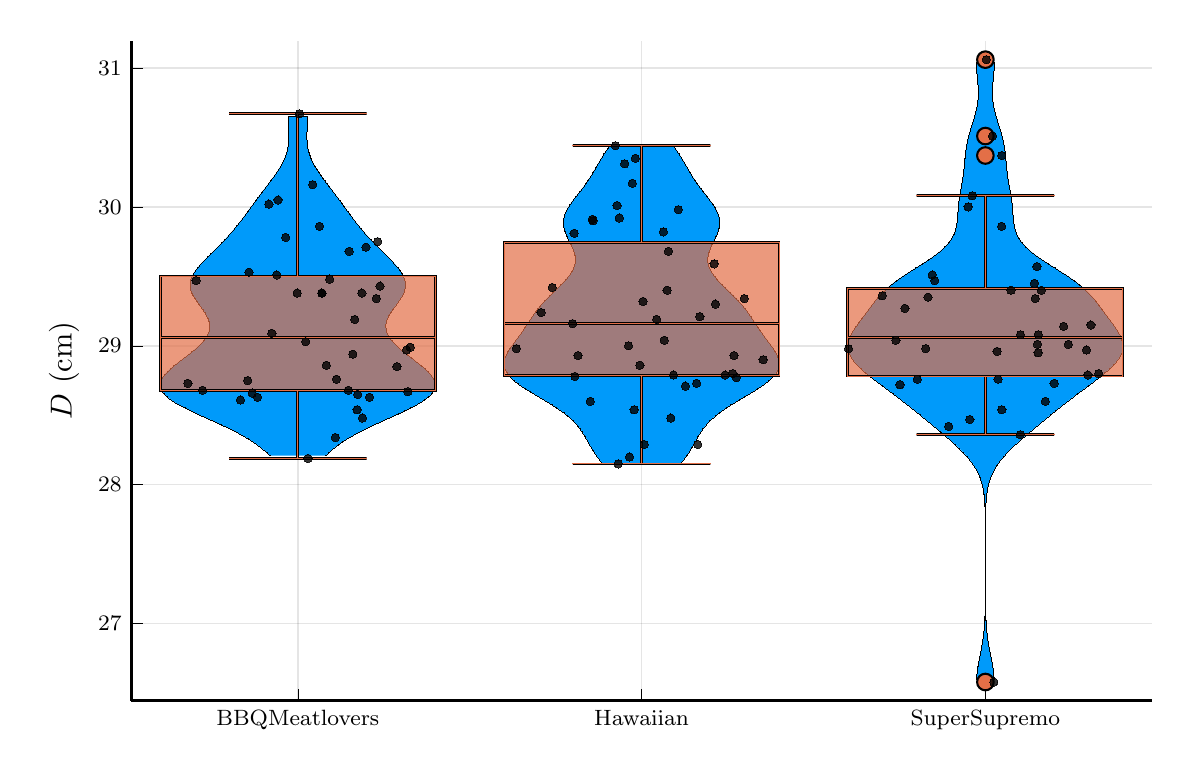
\begin{tikzpicture}[/tikz/background rectangle/.style={fill={rgb,1:red,1.0;green,1.0;blue,1.0}, draw opacity={1.0}}, show background rectangle]
\begin{axis}[point meta max={nan}, point meta min={nan}, title={}, title style={at={{(0.5,1)}}, anchor={south}, font={{\fontsize{14 pt}{18.2 pt}\selectfont}}, color={rgb,1:red,0.0;green,0.0;blue,0.0}, draw opacity={1.0}, rotate={0.0}}, legend style={color={rgb,1:red,0.0;green,0.0;blue,0.0}, draw opacity={1.0}, line width={1}, solid, fill={rgb,1:red,1.0;green,1.0;blue,1.0}, fill opacity={1.0}, text opacity={1.0}, font={{\fontsize{8 pt}{10.4 pt}\selectfont}}, text={rgb,1:red,0.0;green,0.0;blue,0.0}, cells={anchor={center}}, at={(1.02, 1)}, anchor={north west}}, axis background/.style={fill={rgb,1:red,1.0;green,1.0;blue,1.0}, opacity={1.0}}, anchor={north west}, xshift={1.0mm}, yshift={-1.0mm}, width={145.4mm}, height={99.6mm}, scaled x ticks={false}, xlabel={}, x tick style={color={rgb,1:red,0.0;green,0.0;blue,0.0}, opacity={1.0}}, x tick label style={color={rgb,1:red,0.0;green,0.0;blue,0.0}, opacity={1.0}, rotate={0}}, xlabel style={at={(ticklabel cs:0.5)}, anchor=near ticklabel, at={{(ticklabel cs:0.5)}}, anchor={near ticklabel}, font={{\fontsize{11 pt}{14.3 pt}\selectfont}}, color={rgb,1:red,0.0;green,0.0;blue,0.0}, draw opacity={1.0}, rotate={0.0}}, xmajorgrids={true}, xmin={0.015999999999999986}, xmax={2.984}, xtick={{0.5,1.5,2.5}}, xticklabels={{BBQMeatlovers,Hawaiian,SuperSupremo}}, xtick align={inside}, xticklabel style={font={{\fontsize{8 pt}{10.4 pt}\selectfont}}, color={rgb,1:red,0.0;green,0.0;blue,0.0}, draw opacity={1.0}, rotate={0.0}}, x grid style={color={rgb,1:red,0.0;green,0.0;blue,0.0}, draw opacity={0.1}, line width={0.5}, solid}, axis x line*={left}, x axis line style={color={rgb,1:red,0.0;green,0.0;blue,0.0}, draw opacity={1.0}, line width={1}, solid}, scaled y ticks={false}, ylabel={$D$ (cm)}, y tick style={color={rgb,1:red,0.0;green,0.0;blue,0.0}, opacity={1.0}}, y tick label style={color={rgb,1:red,0.0;green,0.0;blue,0.0}, opacity={1.0}, rotate={0}}, ylabel style={at={(ticklabel cs:0.5)}, anchor=near ticklabel, at={{(ticklabel cs:0.5)}}, anchor={near ticklabel}, font={{\fontsize{11 pt}{14.3 pt}\selectfont}}, color={rgb,1:red,0.0;green,0.0;blue,0.0}, draw opacity={1.0}, rotate={0.0}}, ymajorgrids={true}, ymin={26.4456}, ymax={31.194399999999998}, ytick={{27.0,28.0,29.0,30.0,31.0}}, yticklabels={{$27$,$28$,$29$,$30$,$31$}}, ytick align={inside}, yticklabel style={font={{\fontsize{8 pt}{10.4 pt}\selectfont}}, color={rgb,1:red,0.0;green,0.0;blue,0.0}, draw opacity={1.0}, rotate={0.0}}, y grid style={color={rgb,1:red,0.0;green,0.0;blue,0.0}, draw opacity={0.1}, line width={0.5}, solid}, axis y line*={left}, y axis line style={color={rgb,1:red,0.0;green,0.0;blue,0.0}, draw opacity={1.0}, line width={1}, solid}, colorbar={false}]
    \addplot[color={rgb,1:red,0.0;green,0.0;blue,0.0}, name path={35ee40e9-8975-41a1-ba20-418ef8d35794}, area legend, fill={rgb,1:red,0.0;green,0.6056;blue,0.9787}, fill opacity={1.0}, draw opacity={1.0}, line width={0}, solid, forget plot]
        table[row sep={\\}]
        {
            \\
            0.5808586447955323  28.20957568305822  \\
            0.5892457149471652  28.22974798581759  \\
            0.5983905229957045  28.249920288576956  \\
            0.6083661137334528  28.270092591336326  \\
            0.6192398954145399  28.290264894095692  \\
            0.6310677329736953  28.310437196855062  \\
            0.6438875186536965  28.33060949961443  \\
            0.6577126044497048  28.3507818023738  \\
            0.6725255525596723  28.370954105133166  \\
            0.6882727034006926  28.391126407892536  \\
            0.7048600675142893  28.411298710651902  \\
            0.7221510120164515  28.431471013411272  \\
            0.7399661317259506  28.45164331617064  \\
            0.7580855715080977  28.47181561893001  \\
            0.776253906129377  28.491987921689375  \\
            0.7941874980561943  28.512160224448746  \\
            0.8115840571438406  28.532332527208112  \\
            0.8281339368077583  28.552504829967482  \\
            0.8435325378544489  28.57267713272685  \\
            0.8574930714711704  28.59284943548622  \\
            0.8697588715590474  28.613021738245585  \\
            0.880114453118064  28.633194041004955  \\
            0.8883945905636828  28.653366343764322  \\
            0.8944908330228498  28.673538646523692  \\
            0.8983550708035424  28.69371094928306  \\
            0.9  28.71388325204243  \\
            0.8994965777746149  28.734055554801795  \\
            0.8969687945120461  28.754227857561165  \\
            0.8925862869744207  28.774400160320532  \\
            0.8865554587634487  28.7945724630799  \\
            0.8791098469526683  28.81474476583927  \\
            0.8705004706711434  28.834917068598635  \\
            0.860986821231936  28.855089371358005  \\
            0.8508290148458061  28.87526167411737  \\
            0.8402814456455665  28.895433976876742  \\
            0.8295880709702519  28.91560627963611  \\
            0.8189792569288113  28.93577858239548  \\
            0.8086699336236569  28.955950885154845  \\
            0.7988586759470713  28.976123187914215  \\
            0.7897272516847715  28.99629549067358  \\
            0.7814401706501093  29.016467793432952  \\
            0.7741438257698809  29.03664009619232  \\
            0.7679649309475161  29.05681239895169  \\
            0.7630081162210567  29.076984701711055  \\
            0.7593527186599395  29.097157004470425  \\
            0.7570489856591305  29.11732930722979  \\
            0.7561140638860514  29.13750160998916  \\
            0.7565282626347396  29.15767391274853  \\
            0.7582321397848681  29.1778462155079  \\
            0.7611249531261499  29.198018518267265  \\
            0.7650649477755147  29.218190821026635  \\
            0.7698718174251706  29.238363123786  \\
            0.7753314956997097  29.25853542654537  \\
            0.7812032220724969  29.278707729304738  \\
            0.7872286064753771  29.29888003206411  \\
            0.7931422113049867  29.319052334823475  \\
            0.7986830013493683  29.339224637582845  \\
            0.8036059001247342  29.35939694034221  \\
            0.8076926484954441  29.37956924310158  \\
            0.8107611943105706  29.399741545860948  \\
            0.8126729481576266  29.419913848620318  \\
            0.813337410283447  29.440086151379685  \\
            0.8127138903798063  29.460258454139055  \\
            0.8108102832597656  29.48043075689842  \\
            0.8076791047701914  29.50060305965779  \\
            0.8034112090435681  29.520775362417158  \\
            0.7981277787900503  29.540947665176528  \\
            0.7919712885987116  29.561119967935895  \\
            0.7850961782273279  29.581292270695265  \\
            0.7776599378473703  29.60146457345463  \\
            0.7698152074804832  29.621636876214  \\
            0.7617033427029036  29.641809178973368  \\
            0.7534497174427419  29.661981481732738  \\
            0.7451608442224095  29.682153784492105  \\
            0.7369232141493763  29.702326087251475  \\
            0.7288036121181096  29.72249839001084  \\
            0.7208505608168381  29.74267069277021  \\
            0.7130964975518479  29.762842995529578  \\
            0.7055602909620122  29.783015298288948  \\
            0.698249754200422  29.803187601048315  \\
            0.6911638956123503  29.823359903807685  \\
            0.68429475241779  29.84353220656705  \\
            0.6776287612736713  29.86370450932642  \\
            0.6711477167111175  29.883876812085788  \\
            0.6648294421160916  29.904049114845158  \\
            0.6586483402711918  29.924221417604524  \\
            0.6525759986475379  29.944393720363895  \\
            0.6465820007531036  29.96456602312326  \\
            0.640635045291401  29.98473832588263  \\
            0.6347044090623462  30.004910628641998  \\
            0.628761718312478  30.025082931401368  \\
            0.6227829273349723  30.045255234160734  \\
            0.6167503516592183  30.065427536920105  \\
            0.6106545725991465  30.08559983967947  \\
            0.6044960233904246  30.105772142438838  \\
            0.5982860843718172  30.125944445198208  \\
            0.5920475523489541  30.146116747957574  \\
            0.5858144018162725  30.166289050716944  \\
            0.5796308161765656  30.18646135347631  \\
            0.5735495282722202  30.20663365623568  \\
            0.5676295648783237  30.226805958995048  \\
            0.5619335341642168  30.246978261754418  \\
            0.5565246252286562  30.267150564513784  \\
            0.5514635033786165  30.287322867273154  \\
            0.54680528442495  30.30749517003252  \\
            0.5425967579451954  30.32766747279189  \\
            0.5388740061883149  30.347839775551257  \\
            0.5356605354133573  30.368012078310628  \\
            0.5329660031673396  30.388184381069994  \\
            0.5307855909915685  30.408356683829364  \\
            0.5291000392296155  30.42852898658873  \\
            0.5278763301438454  30.4487012893481  \\
            0.5270689779250937  30.468873592107467  \\
            0.5266218594768243  30.489045894866837  \\
            0.5264704980103833  30.509218197626204  \\
            0.5265446925695582  30.529390500385574  \\
            0.5267713709921308  30.54956280314494  \\
            0.5270775322758292  30.56973510590431  \\
            0.5273931379238416  30.589907408663677  \\
            0.5276538118094011  30.610079711423047  \\
            0.5278032154932291  30.630252014182414  \\
            0.527794981397253  30.650424316941784  \\
            0.472205018602747  30.650424316941784  \\
            0.472196784506771  30.630252014182414  \\
            0.47234618819059887  30.610079711423047  \\
            0.47260686207615843  30.589907408663677  \\
            0.4729224677241708  30.56973510590431  \\
            0.47322862900786916  30.54956280314494  \\
            0.4734553074304418  30.529390500385574  \\
            0.47352950198961674  30.509218197626204  \\
            0.4733781405231758  30.489045894866837  \\
            0.47293102207490634  30.468873592107467  \\
            0.4721236698561546  30.4487012893481  \\
            0.4708999607703846  30.42852898658873  \\
            0.46921440900843153  30.408356683829364  \\
            0.4670339968326605  30.388184381069994  \\
            0.4643394645866426  30.368012078310628  \\
            0.46112599381168506  30.347839775551257  \\
            0.4574032420548047  30.32766747279189  \\
            0.4531947155750499  30.30749517003252  \\
            0.44853649662138356  30.287322867273154  \\
            0.44347537477134374  30.267150564513784  \\
            0.43806646583578324  30.246978261754418  \\
            0.4323704351216762  30.226805958995048  \\
            0.42645047172777983  30.20663365623568  \\
            0.4203691838234343  30.18646135347631  \\
            0.41418559818372747  30.166289050716944  \\
            0.40795244765104594  30.146116747957574  \\
            0.40171391562818276  30.125944445198208  \\
            0.3955039766095753  30.105772142438838  \\
            0.3893454274008535  30.08559983967947  \\
            0.3832496483407817  30.065427536920105  \\
            0.3772170726650277  30.045255234160734  \\
            0.37123828168752204  30.025082931401368  \\
            0.3652955909376538  30.004910628641998  \\
            0.35936495470859897  29.98473832588263  \\
            0.35341799924689643  29.96456602312326  \\
            0.3474240013524621  29.944393720363895  \\
            0.3413516597288082  29.924221417604524  \\
            0.33517055788390837  29.904049114845158  \\
            0.32885228328888255  29.883876812085788  \\
            0.3223712387263287  29.86370450932642  \\
            0.31570524758220997  29.84353220656705  \\
            0.3088361043876498  29.823359903807685  \\
            0.301750245799578  29.803187601048315  \\
            0.29443970903798783  29.783015298288948  \\
            0.2869035024481521  29.762842995529578  \\
            0.27914943918316193  29.74267069277021  \\
            0.2711963878818904  29.72249839001084  \\
            0.26307678585062366  29.702326087251475  \\
            0.25483915577759053  29.682153784492105  \\
            0.24655028255725803  29.661981481732738  \\
            0.23829665729709643  29.641809178973368  \\
            0.23018479251951685  29.621636876214  \\
            0.22234006215262975  29.60146457345463  \\
            0.2149038217726721  29.581292270695265  \\
            0.20802871140128837  29.561119967935895  \\
            0.2018722212099498  29.540947665176528  \\
            0.1965887909564319  29.520775362417158  \\
            0.1923208952298086  29.50060305965779  \\
            0.18918971674023444  29.48043075689842  \\
            0.1872861096201937  29.460258454139055  \\
            0.18666258971655297  29.440086151379685  \\
            0.18732705184237342  29.419913848620318  \\
            0.18923880568942936  29.399741545860948  \\
            0.19230735150455597  29.37956924310158  \\
            0.19639409987526574  29.35939694034221  \\
            0.20131699865063168  29.339224637582845  \\
            0.20685778869501326  29.319052334823475  \\
            0.21277139352462288  29.29888003206411  \\
            0.21879677792750302  29.278707729304738  \\
            0.22466850430029023  29.25853542654537  \\
            0.2301281825748293  29.238363123786  \\
            0.23493505222448535  29.218190821026635  \\
            0.23887504687385003  29.198018518267265  \\
            0.24176786021513186  29.1778462155079  \\
            0.24347173736526045  29.15767391274853  \\
            0.2438859361139486  29.13750160998916  \\
            0.24295101434086952  29.11732930722979  \\
            0.24064728134006053  29.097157004470425  \\
            0.23699188377894337  29.076984701711055  \\
            0.232035069052484  29.05681239895169  \\
            0.22585617423011906  29.03664009619232  \\
            0.21855982934989077  29.016467793432952  \\
            0.2102727483152284  28.99629549067358  \\
            0.20114132405292873  28.976123187914215  \\
            0.1913300663763431  28.955950885154845  \\
            0.18102074307118865  28.93577858239548  \\
            0.1704119290297481  28.91560627963611  \\
            0.1597185543544335  28.895433976876742  \\
            0.1491709851541939  28.87526167411737  \\
            0.13901317876806396  28.855089371358005  \\
            0.1294995293288566  28.834917068598635  \\
            0.12089015304733175  28.81474476583927  \\
            0.11344454123655134  28.7945724630799  \\
            0.10741371302557934  28.774400160320532  \\
            0.10303120548795386  28.754227857561165  \\
            0.10050342222538511  28.734055554801795  \\
            0.09999999999999998  28.71388325204243  \\
            0.10164492919645762  28.69371094928306  \\
            0.10550916697715013  28.673538646523692  \\
            0.1116054094363172  28.653366343764322  \\
            0.11988554688193598  28.633194041004955  \\
            0.13024112844095265  28.613021738245585  \\
            0.14250692852882968  28.59284943548622  \\
            0.15646746214555107  28.57267713272685  \\
            0.17186606319224174  28.552504829967482  \\
            0.18841594285615937  28.532332527208112  \\
            0.20581250194380568  28.512160224448746  \\
            0.2237460938706231  28.491987921689375  \\
            0.24191442849190226  28.47181561893001  \\
            0.2600338682740494  28.45164331617064  \\
            0.2778489879835485  28.431471013411272  \\
            0.29513993248571074  28.411298710651902  \\
            0.3117272965993075  28.391126407892536  \\
            0.3274744474403277  28.370954105133166  \\
            0.3422873955502952  28.3507818023738  \\
            0.35611248134630347  28.33060949961443  \\
            0.36893226702630466  28.310437196855062  \\
            0.38076010458546  28.290264894095692  \\
            0.3916338862665472  28.270092591336326  \\
            0.4016094770042955  28.249920288576956  \\
            0.41075428505283484  28.22974798581759  \\
            0.4191413552044677  28.20957568305822  \\
        }
        ;
    \addplot[color={rgb,1:red,0.0;green,0.0;blue,0.0}, name path={35ee40e9-8975-41a1-ba20-418ef8d35794}, area legend, fill={rgb,1:red,0.0;green,0.6056;blue,0.9787}, fill opacity={1.0}, draw opacity={1.0}, line width={0}, solid, forget plot]
        table[row sep={\\}]
        {
            \\
            1.612765494899509  28.151557031043716  \\
            1.6191558261064962  28.170774559933736  \\
            1.6252040278250304  28.18999208882376  \\
            1.6308900925421819  28.209209617713782  \\
            1.636215725451621  28.228427146603803  \\
            1.6412053598511895  28.247644675493824  \\
            1.6459061036109277  28.266862204383845  \\
            1.6503865868517347  28.28607973327387  \\
            1.6547347409916437  28.30529726216389  \\
            1.6590545954939357  28.32451479105391  \\
            1.6634622271535096  28.343732319943932  \\
            1.6680810348352226  28.362949848833953  \\
            1.6730365388052553  28.382167377723974  \\
            1.6784509181155638  28.401384906614  \\
            1.684437503060158  28.42060243550402  \\
            1.691095434538794  28.43981996439404  \\
            1.6985046906732435  28.45903749328406  \\
            1.7067216655785797  28.478255022174082  \\
            1.715775467622276  28.497472551064103  \\
            1.7256650857783318  28.516690079954127  \\
            1.7363575527793849  28.53590760884415  \\
            1.7477872117442095  28.55512513773417  \\
            1.7598561672257809  28.57434266662419  \\
            1.7724359703924935  28.59356019551421  \\
            1.785370549834469  28.612777724404236  \\
            1.7984803535990102  28.631995253294257  \\
            1.8115676150300288  28.651212782184277  \\
            1.8244225967610692  28.6704303110743  \\
            1.8368306071403218  28.68964783996432  \\
            1.848579525951016  28.70886536885434  \\
            1.8594675267281437  28.728082897744365  \\
            1.8693106465543725  28.747300426634386  \\
            1.8779498356801274  28.766517955524407  \\
            1.8852571222255485  28.785735484414428  \\
            1.8911405535080483  28.80495301330445  \\
            1.895547625181016  28.824170542194473  \\
            1.8984669803385976  28.843388071084494  \\
            1.8999282491481548  28.862605599974515  \\
            1.9  28.881823128864536  \\
            1.8987858791424836  28.901040657754557  \\
            1.8964191203150118  28.920258186644578  \\
            1.8930557020545105  28.939475715534602  \\
            1.8888665117286916  28.958693244424623  \\
            1.8840289365115797  28.977910773314644  \\
            1.8787183383367418  28.997128302204665  \\
            1.8730998797491405  29.016345831094686  \\
            1.8673211496018116  29.03556335998471  \\
            1.8615059924934871  29.05478088887473  \\
            1.8557498761744018  29.073998417764752  \\
            1.8501170408694132  29.093215946654773  \\
            1.8446395689424373  29.112433475544794  \\
            1.8393183989849646  29.131651004434815  \\
            1.8341261923869197  29.15086853332484  \\
            1.8290118501346408  29.17008606221486  \\
            1.823906380139697  29.18930359110488  \\
            1.8187297372457847  29.208521119994902  \\
            1.8133982043558217  29.227738648884923  \\
            1.8078318573607257  29.246956177774948  \\
            1.8019616602417272  29.26617370666497  \\
            1.7957357692218143  29.28539123555499  \\
            1.789124683401393  29.30460876444501  \\
            1.7821249592643866  29.32382629333503  \\
            1.7747613016037698  29.343043822225052  \\
            1.7670869466274546  29.362261351115077  \\
            1.7591823567482812  29.381478880005098  \\
            1.751152343618133  29.40069640889512  \\
            1.743121820038566  29.41991393778514  \\
            1.735230447608357  29.43913146667516  \\
            1.7276264922878886  29.458348995565185  \\
            1.7204602233676405  29.477566524455206  \\
            1.7138771934329171  29.496784053345227  \\
            1.7080117202924068  29.516001582235248  \\
            1.7029808602011283  29.53521911112527  \\
            1.6988791194844515  29.55443664001529  \\
            1.6957741034124805  29.573654168905314  \\
            1.6937032510130325  29.592871697795335  \\
            1.6926717557046052  29.612089226685356  \\
            1.692651726277032  29.631306755575377  \\
            1.6935826016984106  29.650524284465398  \\
            1.6953727962036569  29.669741813355422  \\
            1.6979025170155744  29.688959342245443  \\
            1.7010276643620834  29.708176871135464  \\
            1.7045846907826046  29.727394400025485  \\
            1.7083962632356102  29.746611928915506  \\
            1.7122775373447712  29.765829457805527  \\
            1.7160428195135056  29.78504698669555  \\
            1.7195123619917412  29.804264515585572  \\
            1.722519011595028  29.823482044475593  \\
            1.7249144184420158  29.842699573365614  \\
            1.7265745105126133  29.861917102255635  \\
            1.7274039560844279  29.88113463114566  \\
            1.72733937098823  29.90035216003568  \\
            1.7263510812618132  29.9195696889257  \\
            1.7244433223775295  29.938787217815722  \\
            1.7216528400435411  29.958004746705743  \\
            1.7180459492186244  29.977222275595764  \\
            1.7137142008045656  29.99643980448579  \\
            1.708768892276696  30.01565733337581  \\
            1.7033347322120296  30.03487486226583  \\
            1.697543023070525  30.05409239115585  \\
            1.691524756972505  30.073309920045872  \\
            1.6854040228619833  30.092527448935897  \\
            1.6792920998563643  30.111744977825918  \\
            1.6732825625304266  30.13096250671594  \\
            1.6674476532129727  30.15018003560596  \\
            1.6618360896201376  30.16939756449598  \\
            1.6564723799989343  30.188615093386  \\
            1.6513576196450723  30.207832622276026  \\
            1.6464716493521365  30.227050151166047  \\
            1.641776374552557  30.246267680056068  \\
            1.6372199789918433  30.26548520894609  \\
            1.6327417226034906  30.28470273783611  \\
            1.6282769919745135  30.30392026672613  \\
            1.6237622737800566  30.323137795616155  \\
            1.6191397454806908  30.342355324506176  \\
            1.6143612205660154  30.361572853396197  \\
            1.609391243624345  30.380790382286218  \\
            1.604209198601177  30.40000791117624  \\
            1.5988103664165683  30.419225440066263  \\
            1.5932059402568464  30.438442968956284  \\
            1.4067940597431536  30.438442968956284  \\
            1.4011896335834317  30.419225440066263  \\
            1.395790801398823  30.40000791117624  \\
            1.390608756375655  30.380790382286218  \\
            1.3856387794339846  30.361572853396197  \\
            1.3808602545193092  30.342355324506176  \\
            1.3762377262199434  30.323137795616155  \\
            1.3717230080254865  30.30392026672613  \\
            1.3672582773965094  30.28470273783611  \\
            1.3627800210081567  30.26548520894609  \\
            1.358223625447443  30.246267680056068  \\
            1.3535283506478635  30.227050151166047  \\
            1.3486423803549277  30.207832622276026  \\
            1.3435276200010657  30.188615093386  \\
            1.3381639103798624  30.16939756449598  \\
            1.3325523467870273  30.15018003560596  \\
            1.3267174374695734  30.13096250671594  \\
            1.3207079001436357  30.111744977825918  \\
            1.3145959771380167  30.092527448935897  \\
            1.308475243027495  30.073309920045872  \\
            1.302456976929475  30.05409239115585  \\
            1.2966652677879704  30.03487486226583  \\
            1.291231107723304  30.01565733337581  \\
            1.2862857991954344  29.99643980448579  \\
            1.2819540507813756  29.977222275595764  \\
            1.2783471599564589  29.958004746705743  \\
            1.2755566776224705  29.938787217815722  \\
            1.2736489187381868  29.9195696889257  \\
            1.27266062901177  29.90035216003568  \\
            1.2725960439155721  29.88113463114566  \\
            1.2734254894873867  29.861917102255635  \\
            1.2750855815579842  29.842699573365614  \\
            1.277480988404972  29.823482044475593  \\
            1.2804876380082588  29.804264515585572  \\
            1.2839571804864944  29.78504698669555  \\
            1.2877224626552288  29.765829457805527  \\
            1.2916037367643898  29.746611928915506  \\
            1.2954153092173954  29.727394400025485  \\
            1.2989723356379166  29.708176871135464  \\
            1.3020974829844256  29.688959342245443  \\
            1.3046272037963431  29.669741813355422  \\
            1.3064173983015894  29.650524284465398  \\
            1.307348273722968  29.631306755575377  \\
            1.3073282442953948  29.612089226685356  \\
            1.3062967489869675  29.592871697795335  \\
            1.3042258965875195  29.573654168905314  \\
            1.3011208805155485  29.55443664001529  \\
            1.2970191397988717  29.53521911112527  \\
            1.2919882797075932  29.516001582235248  \\
            1.2861228065670829  29.496784053345227  \\
            1.2795397766323595  29.477566524455206  \\
            1.2723735077121114  29.458348995565185  \\
            1.264769552391643  29.43913146667516  \\
            1.256878179961434  29.41991393778514  \\
            1.248847656381867  29.40069640889512  \\
            1.2408176432517188  29.381478880005098  \\
            1.2329130533725454  29.362261351115077  \\
            1.2252386983962302  29.343043822225052  \\
            1.2178750407356134  29.32382629333503  \\
            1.210875316598607  29.30460876444501  \\
            1.2042642307781857  29.28539123555499  \\
            1.1980383397582728  29.26617370666497  \\
            1.1921681426392743  29.246956177774948  \\
            1.1866017956441783  29.227738648884923  \\
            1.1812702627542153  29.208521119994902  \\
            1.176093619860303  29.18930359110488  \\
            1.1709881498653592  29.17008606221486  \\
            1.1658738076130803  29.15086853332484  \\
            1.1606816010150354  29.131651004434815  \\
            1.1553604310575627  29.112433475544794  \\
            1.1498829591305868  29.093215946654773  \\
            1.1442501238255982  29.073998417764752  \\
            1.1384940075065129  29.05478088887473  \\
            1.1326788503981884  29.03556335998471  \\
            1.1269001202508595  29.016345831094686  \\
            1.1212816616632582  28.997128302204665  \\
            1.1159710634884203  28.977910773314644  \\
            1.1111334882713084  28.958693244424623  \\
            1.1069442979454895  28.939475715534602  \\
            1.1035808796849882  28.920258186644578  \\
            1.1012141208575164  28.901040657754557  \\
            1.1  28.881823128864536  \\
            1.1000717508518452  28.862605599974515  \\
            1.1015330196614024  28.843388071084494  \\
            1.104452374818984  28.824170542194473  \\
            1.1088594464919517  28.80495301330445  \\
            1.1147428777744515  28.785735484414428  \\
            1.1220501643198726  28.766517955524407  \\
            1.1306893534456275  28.747300426634386  \\
            1.1405324732718563  28.728082897744365  \\
            1.151420474048984  28.70886536885434  \\
            1.1631693928596782  28.68964783996432  \\
            1.1755774032389308  28.6704303110743  \\
            1.1884323849699712  28.651212782184277  \\
            1.2015196464009898  28.631995253294257  \\
            1.214629450165531  28.612777724404236  \\
            1.2275640296075065  28.59356019551421  \\
            1.2401438327742191  28.57434266662419  \\
            1.2522127882557905  28.55512513773417  \\
            1.2636424472206151  28.53590760884415  \\
            1.2743349142216682  28.516690079954127  \\
            1.284224532377724  28.497472551064103  \\
            1.2932783344214203  28.478255022174082  \\
            1.3014953093267565  28.45903749328406  \\
            1.308904565461206  28.43981996439404  \\
            1.315562496939842  28.42060243550402  \\
            1.3215490818844362  28.401384906614  \\
            1.3269634611947447  28.382167377723974  \\
            1.3319189651647774  28.362949848833953  \\
            1.3365377728464904  28.343732319943932  \\
            1.3409454045060643  28.32451479105391  \\
            1.3452652590083563  28.30529726216389  \\
            1.3496134131482653  28.28607973327387  \\
            1.3540938963890723  28.266862204383845  \\
            1.3587946401488105  28.247644675493824  \\
            1.363784274548379  28.228427146603803  \\
            1.3691099074578181  28.209209617713782  \\
            1.3747959721749696  28.18999208882376  \\
            1.3808441738935038  28.170774559933736  \\
            1.387234505100491  28.151557031043716  \\
        }
        ;
    \addplot[color={rgb,1:red,0.0;green,0.0;blue,0.0}, name path={35ee40e9-8975-41a1-ba20-418ef8d35794}, area legend, fill={rgb,1:red,0.0;green,0.6056;blue,0.9787}, fill opacity={1.0}, draw opacity={1.0}, line width={0}, solid, forget plot]
        table[row sep={\\}]
        {
            \\
            2.525598998510192  26.598642279849745  \\
            2.5249024242950004  26.628864833865396  \\
            2.5236341124198005  26.659087387881044  \\
            2.5218834763704656  26.689309941896695  \\
            2.5197684672332086  26.719532495912343  \\
            2.517422466742593  26.749755049927995  \\
            2.5149805078379437  26.779977603943642  \\
            2.5125667777830754  26.810200157959294  \\
            2.510284947666048  26.84042271197494  \\
            2.508212232053958  26.870645265990593  \\
            2.506397370759539  26.900867820006244  \\
            2.5048620922756117  26.931090374021892  \\
            2.5036051754656836  26.961312928037543  \\
            2.5026080222822378  26.99153548205319  \\
            2.5018406787366625  27.021758036068842  \\
            2.5012674376589805  27.05198059008449  \\
            2.5008514462164717  27.08220314410014  \\
            2.500558045881076  27.11242569811579  \\
            2.500356832781047  27.14264825213144  \\
            2.50022260857798  27.17287080614709  \\
            2.5001354883515483  27.20309336016274  \\
            2.500080453973503  27.23331591417839  \\
            2.500046611131125  27.26353846819404  \\
            2.5000263497609523  27.29376102220969  \\
            2.500014541788867  27.323983576225338  \\
            2.500007850861737  27.35420613024099  \\
            2.5000041835235396  27.384428684256637  \\
            2.5000022819039875  27.41465123827229  \\
            2.5000014428626787  27.444873792287936  \\
            2.5000013445382407  27.475096346303587  \\
            2.500001965133116  27.505318900319235  \\
            2.5000035879154447  27.535541454334886  \\
            2.5000068990918107  27.565764008350534  \\
            2.500013200271038  27.595986562366186  \\
            2.5000247736627186  27.626209116381837  \\
            2.500045454296182  27.656431670397485  \\
            2.5000814764573995  27.686654224413136  \\
            2.5001426664252526  27.716876778428784  \\
            2.500244043690815  27.747099332444435  \\
            2.5004078600936945  27.777321886460083  \\
            2.500666043003474  27.807544440475734  \\
            2.501062910315703  27.837766994491382  \\
            2.501657894089207  27.867989548507033  \\
            2.502527859438812  27.89821210252268  \\
            2.5037684626138503  27.928434656538332  \\
            2.5054938969655787  27.958657210553984  \\
            2.50783437580184  27.98887976456963  \\
            2.510930842741178  28.019102318585283  \\
            2.514926711683559  28.04932487260093  \\
            2.5199569147913805  28.079547426616582  \\
            2.5261351261736853  28.10976998063223  \\
            2.5335406294981873  28.13999253464788  \\
            2.5422067688256362  28.17021508866353  \\
            2.552113111399731  28.20043764267918  \\
            2.563183235556329  28.230660196694828  \\
            2.5752893856803665  28.26088275071048  \\
            2.588264165461145  28.29110530472613  \\
            2.6019181440291637  28.32132785874178  \\
            2.6160609943744713  28.35155041275743  \\
            2.6305228737861435  28.381772966773077  \\
            2.645172451816341  28.41199552078873  \\
            2.659928425952656  28.442218074804376  \\
            2.6747624890870405  28.472440628820028  \\
            2.6896932856864195  28.502663182835676  \\
            2.7047725373965306  28.532885736851327  \\
            2.7200658231646186  28.563108290866975  \\
            2.7356311487649574  28.593330844882626  \\
            2.7514983244704747  28.623553398898274  \\
            2.767651426050969  28.653775952913925  \\
            2.7840155903212436  28.683998506929576  \\
            2.8004485233783902  28.714221060945224  \\
            2.816736724114642  28.744443614960876  \\
            2.832596658095178  28.774666168976523  \\
            2.847681761421792  28.804888722992175  \\
            2.8615967583769035  28.835111277007822  \\
            2.8739207978053822  28.865333831023474  \\
            2.8842399474699243  28.89555638503912  \\
            2.8921875745704253  28.925778939054773  \\
            2.897488469135147  28.95600149307042  \\
            2.9  28.986224047086072  \\
            2.899742056805747  29.016446601101723  \\
            2.8969078052199957  29.04666915511737  \\
            2.8918497061699173  29.076891709133022  \\
            2.885039551589299  29.10711426314867  \\
            2.877006582481274  29.13733681716432  \\
            2.8682628271747315  29.16755937117997  \\
            2.859228328976979  29.19778192519562  \\
            2.8501699423918616  29.22800447921127  \\
            2.8411654837854865  29.25822703322692  \\
            2.8321005541182886  29.288449587242567  \\
            2.8226992615831072  29.31867214125822  \\
            2.8125836894490233  29.348894695273867  \\
            2.8013516456930807  29.379117249289518  \\
            2.7886590718715007  29.40933980330517  \\
            2.774293030041459  29.439562357320817  \\
            2.758223366910986  29.46978491133647  \\
            2.7406253662964666  29.500007465352116  \\
            2.7218709775720993  29.530230019367767  \\
            2.7024914695512616  29.560452573383415  \\
            2.6831186536355087  29.590675127399066  \\
            2.6644144995267642  29.620897681414714  \\
            2.646999773809122  29.651120235430366  \\
            2.6313913878338857  29.681342789446013  \\
            2.6179558598132386  29.711565343461665  \\
            2.60688325111464  29.741787897477316  \\
            2.598182726042671  29.772010451492964  \\
            2.591698014251816  29.802233005508615  \\
            2.5871388682710306  29.832455559524263  \\
            2.5841232616191583  29.862678113539914  \\
            2.582224555647465  29.892900667555562  \\
            2.5810180500448783  29.923123221571213  \\
            2.580122044108535  29.95334577558686  \\
            2.579229596518254  29.983568329602512  \\
            2.5781284392064547  30.01379088361816  \\
            2.576707876799305  30.04401343763381  \\
            2.5749529128507826  30.074235991649463  \\
            2.572927210294095  30.10445854566511  \\
            2.570747712219684  30.134681099680762  \\
            2.5685546850123564  30.16490365369641  \\
            2.5664814521834973  30.19512620771206  \\
            2.5646280445396195  30.22534876172771  \\
            2.563042353352286  30.25557131574336  \\
            2.561711195301141  30.285793869759008  \\
            2.5605621493371125  30.31601642377466  \\
            2.5594753596638933  30.346238977790307  \\
            2.5583030026625226  30.37646153180596  \\
            2.55689304586384  30.406684085821606  \\
            2.5551134544909786  30.436906639837257  \\
            2.5528731748259914  30.46712919385291  \\
            2.5501369670936973  30.497351747868557  \\
            2.546932296179258  30.527574301884208  \\
            2.543347783472259  30.557796855899856  \\
            2.5395239427448653  30.588019409915507  \\
            2.5356378785975378  30.618241963931155  \\
            2.5318842072192385  30.648464517946806  \\
            2.5284546444524834  30.678687071962454  \\
            2.525518551742064  30.708909625978105  \\
            2.523206342794094  30.739132179993753  \\
            2.521597152775446  30.769354734009404  \\
            2.5207116573267068  30.799577288025056  \\
            2.5205104573102872  30.829799842040703  \\
            2.5208980263152347  30.860022396056355  \\
            2.521731827104502  30.890244950072002  \\
            2.522835809045504  30.920467504087654  \\
            2.524017091587566  30.9506900581033  \\
            2.5250842504788187  30.980912612118953  \\
            2.525865326630911  31.0111351661346  \\
            2.5262235669380826  31.041357720150252  \\
            2.4737764330619174  31.041357720150252  \\
            2.474134673369089  31.0111351661346  \\
            2.4749157495211813  30.980912612118953  \\
            2.475982908412434  30.9506900581033  \\
            2.477164190954496  30.920467504087654  \\
            2.478268172895498  30.890244950072002  \\
            2.4791019736847653  30.860022396056355  \\
            2.4794895426897128  30.829799842040703  \\
            2.4792883426732932  30.799577288025056  \\
            2.478402847224554  30.769354734009404  \\
            2.476793657205906  30.739132179993753  \\
            2.474481448257936  30.708909625978105  \\
            2.4715453555475166  30.678687071962454  \\
            2.4681157927807615  30.648464517946806  \\
            2.4643621214024622  30.618241963931155  \\
            2.4604760572551347  30.588019409915507  \\
            2.456652216527741  30.557796855899856  \\
            2.453067703820742  30.527574301884208  \\
            2.4498630329063027  30.497351747868557  \\
            2.4471268251740086  30.46712919385291  \\
            2.4448865455090214  30.436906639837257  \\
            2.44310695413616  30.406684085821606  \\
            2.4416969973374774  30.37646153180596  \\
            2.4405246403361067  30.346238977790307  \\
            2.4394378506628875  30.31601642377466  \\
            2.438288804698859  30.285793869759008  \\
            2.436957646647714  30.25557131574336  \\
            2.4353719554603805  30.22534876172771  \\
            2.4335185478165027  30.19512620771206  \\
            2.4314453149876436  30.16490365369641  \\
            2.429252287780316  30.134681099680762  \\
            2.427072789705905  30.10445854566511  \\
            2.4250470871492174  30.074235991649463  \\
            2.423292123200695  30.04401343763381  \\
            2.4218715607935453  30.01379088361816  \\
            2.420770403481746  29.983568329602512  \\
            2.419877955891465  29.95334577558686  \\
            2.4189819499551217  29.923123221571213  \\
            2.417775444352535  29.892900667555562  \\
            2.4158767383808417  29.862678113539914  \\
            2.4128611317289694  29.832455559524263  \\
            2.408301985748184  29.802233005508615  \\
            2.401817273957329  29.772010451492964  \\
            2.39311674888536  29.741787897477316  \\
            2.3820441401867614  29.711565343461665  \\
            2.3686086121661143  29.681342789446013  \\
            2.353000226190878  29.651120235430366  \\
            2.3355855004732358  29.620897681414714  \\
            2.3168813463644913  29.590675127399066  \\
            2.2975085304487384  29.560452573383415  \\
            2.2781290224279007  29.530230019367767  \\
            2.2593746337035334  29.500007465352116  \\
            2.241776633089014  29.46978491133647  \\
            2.225706969958541  29.439562357320817  \\
            2.2113409281284993  29.40933980330517  \\
            2.1986483543069193  29.379117249289518  \\
            2.1874163105509767  29.348894695273867  \\
            2.1773007384168928  29.31867214125822  \\
            2.1678994458817114  29.288449587242567  \\
            2.1588345162145135  29.25822703322692  \\
            2.1498300576081384  29.22800447921127  \\
            2.140771671023021  29.19778192519562  \\
            2.1317371728252685  29.16755937117997  \\
            2.122993417518726  29.13733681716432  \\
            2.114960448410701  29.10711426314867  \\
            2.1081502938300827  29.076891709133022  \\
            2.1030921947800043  29.04666915511737  \\
            2.100257943194253  29.016446601101723  \\
            2.1  28.986224047086072  \\
            2.102511530864853  28.95600149307042  \\
            2.1078124254295747  28.925778939054773  \\
            2.1157600525300757  28.89555638503912  \\
            2.1260792021946178  28.865333831023474  \\
            2.1384032416230965  28.835111277007822  \\
            2.152318238578208  28.804888722992175  \\
            2.167403341904822  28.774666168976523  \\
            2.183263275885358  28.744443614960876  \\
            2.1995514766216098  28.714221060945224  \\
            2.2159844096787564  28.683998506929576  \\
            2.232348573949031  28.653775952913925  \\
            2.2485016755295253  28.623553398898274  \\
            2.2643688512350426  28.593330844882626  \\
            2.2799341768353814  28.563108290866975  \\
            2.2952274626034694  28.532885736851327  \\
            2.3103067143135805  28.502663182835676  \\
            2.3252375109129595  28.472440628820028  \\
            2.340071574047344  28.442218074804376  \\
            2.354827548183659  28.41199552078873  \\
            2.3694771262138565  28.381772966773077  \\
            2.3839390056255287  28.35155041275743  \\
            2.3980818559708363  28.32132785874178  \\
            2.411735834538855  28.29110530472613  \\
            2.4247106143196335  28.26088275071048  \\
            2.436816764443671  28.230660196694828  \\
            2.447886888600269  28.20043764267918  \\
            2.4577932311743638  28.17021508866353  \\
            2.4664593705018127  28.13999253464788  \\
            2.4738648738263147  28.10976998063223  \\
            2.4800430852086195  28.079547426616582  \\
            2.485073288316441  28.04932487260093  \\
            2.489069157258822  28.019102318585283  \\
            2.49216562419816  27.98887976456963  \\
            2.4945061030344213  27.958657210553984  \\
            2.4962315373861497  27.928434656538332  \\
            2.497472140561188  27.89821210252268  \\
            2.498342105910793  27.867989548507033  \\
            2.498937089684297  27.837766994491382  \\
            2.499333956996526  27.807544440475734  \\
            2.4995921399063055  27.777321886460083  \\
            2.499755956309185  27.747099332444435  \\
            2.4998573335747474  27.716876778428784  \\
            2.4999185235426005  27.686654224413136  \\
            2.499954545703818  27.656431670397485  \\
            2.4999752263372814  27.626209116381837  \\
            2.499986799728962  27.595986562366186  \\
            2.4999931009081893  27.565764008350534  \\
            2.4999964120845553  27.535541454334886  \\
            2.499998034866884  27.505318900319235  \\
            2.4999986554617593  27.475096346303587  \\
            2.4999985571373213  27.444873792287936  \\
            2.4999977180960125  27.41465123827229  \\
            2.4999958164764604  27.384428684256637  \\
            2.499992149138263  27.35420613024099  \\
            2.499985458211133  27.323983576225338  \\
            2.4999736502390477  27.29376102220969  \\
            2.499953388868875  27.26353846819404  \\
            2.499919546026497  27.23331591417839  \\
            2.4998645116484517  27.20309336016274  \\
            2.49977739142202  27.17287080614709  \\
            2.499643167218953  27.14264825213144  \\
            2.499441954118924  27.11242569811579  \\
            2.4991485537835283  27.08220314410014  \\
            2.4987325623410195  27.05198059008449  \\
            2.4981593212633375  27.021758036068842  \\
            2.4973919777177622  26.99153548205319  \\
            2.4963948245343164  26.961312928037543  \\
            2.4951379077243883  26.931090374021892  \\
            2.493602629240461  26.900867820006244  \\
            2.491787767946042  26.870645265990593  \\
            2.489715052333952  26.84042271197494  \\
            2.4874332222169246  26.810200157959294  \\
            2.4850194921620563  26.779977603943642  \\
            2.482577533257407  26.749755049927995  \\
            2.4802315327667914  26.719532495912343  \\
            2.4781165236295344  26.689309941896695  \\
            2.4763658875801995  26.659087387881044  \\
            2.4750975757049996  26.628864833865396  \\
            2.474401001489808  26.598642279849745  \\
        }
        ;
    \addplot[color={rgb,1:red,0.0;green,0.0;blue,0.0}, name path={90c5b4d8-5545-4c20-bcb7-2b46a109e84e}, area legend, fill={rgb,1:red,0.8889;green,0.4356;blue,0.2781}, fill opacity={0.7}, draw opacity={1.0}, line width={1}, solid, forget plot]
        table[row sep={\\}]
        {
            \\
            0.5  28.19  \\
            0.3  28.19  \\
            0.7  28.19  \\
            0.5  28.19  \\
            0.5  28.68  \\
        }
        ;
    \addplot[color={rgb,1:red,0.0;green,0.0;blue,0.0}, name path={90c5b4d8-5545-4c20-bcb7-2b46a109e84e}, area legend, fill={rgb,1:red,0.8889;green,0.4356;blue,0.2781}, fill opacity={0.7}, draw opacity={1.0}, line width={1}, solid, forget plot]
        table[row sep={\\}]
        {
            \\
            0.9  28.68  \\
            0.9  29.060000000000002  \\
            0.09999999999999998  29.060000000000002  \\
            0.09999999999999998  28.68  \\
            0.9  28.68  \\
            0.9  29.060000000000002  \\
        }
        ;
    \addplot[color={rgb,1:red,0.0;green,0.0;blue,0.0}, name path={90c5b4d8-5545-4c20-bcb7-2b46a109e84e}, area legend, fill={rgb,1:red,0.8889;green,0.4356;blue,0.2781}, fill opacity={0.7}, draw opacity={1.0}, line width={1}, solid, forget plot]
        table[row sep={\\}]
        {
            \\
            0.9  29.5025  \\
            0.09999999999999998  29.5025  \\
            0.09999999999999998  29.060000000000002  \\
            0.9  29.060000000000002  \\
            0.9  29.5025  \\
            0.5  29.5025  \\
        }
        ;
    \addplot[color={rgb,1:red,0.0;green,0.0;blue,0.0}, name path={90c5b4d8-5545-4c20-bcb7-2b46a109e84e}, area legend, fill={rgb,1:red,0.8889;green,0.4356;blue,0.2781}, fill opacity={0.7}, draw opacity={1.0}, line width={1}, solid, forget plot]
        table[row sep={\\}]
        {
            \\
            0.5  30.67  \\
            0.3  30.67  \\
            0.7  30.67  \\
            0.5  30.67  \\
            0.5  29.5025  \\
        }
        ;
    \addplot[color={rgb,1:red,0.0;green,0.0;blue,0.0}, name path={90c5b4d8-5545-4c20-bcb7-2b46a109e84e}, area legend, fill={rgb,1:red,0.8889;green,0.4356;blue,0.2781}, fill opacity={0.7}, draw opacity={1.0}, line width={1}, solid, forget plot]
        table[row sep={\\}]
        {
            \\
            1.5  28.15  \\
            1.3  28.15  \\
            1.7  28.15  \\
            1.5  28.15  \\
            1.5  28.785  \\
        }
        ;
    \addplot[color={rgb,1:red,0.0;green,0.0;blue,0.0}, name path={90c5b4d8-5545-4c20-bcb7-2b46a109e84e}, area legend, fill={rgb,1:red,0.8889;green,0.4356;blue,0.2781}, fill opacity={0.7}, draw opacity={1.0}, line width={1}, solid, forget plot]
        table[row sep={\\}]
        {
            \\
            1.9  28.785  \\
            1.9  29.16  \\
            1.1  29.16  \\
            1.1  28.785  \\
            1.9  28.785  \\
            1.9  29.16  \\
        }
        ;
    \addplot[color={rgb,1:red,0.0;green,0.0;blue,0.0}, name path={90c5b4d8-5545-4c20-bcb7-2b46a109e84e}, area legend, fill={rgb,1:red,0.8889;green,0.4356;blue,0.2781}, fill opacity={0.7}, draw opacity={1.0}, line width={1}, solid, forget plot]
        table[row sep={\\}]
        {
            \\
            1.9  29.744999999999997  \\
            1.1  29.744999999999997  \\
            1.1  29.16  \\
            1.9  29.16  \\
            1.9  29.744999999999997  \\
            1.5  29.744999999999997  \\
        }
        ;
    \addplot[color={rgb,1:red,0.0;green,0.0;blue,0.0}, name path={90c5b4d8-5545-4c20-bcb7-2b46a109e84e}, area legend, fill={rgb,1:red,0.8889;green,0.4356;blue,0.2781}, fill opacity={0.7}, draw opacity={1.0}, line width={1}, solid, forget plot]
        table[row sep={\\}]
        {
            \\
            1.5  30.44  \\
            1.3  30.44  \\
            1.7  30.44  \\
            1.5  30.44  \\
            1.5  29.744999999999997  \\
        }
        ;
    \addplot[color={rgb,1:red,0.0;green,0.0;blue,0.0}, name path={90c5b4d8-5545-4c20-bcb7-2b46a109e84e}, area legend, fill={rgb,1:red,0.8889;green,0.4356;blue,0.2781}, fill opacity={0.7}, draw opacity={1.0}, line width={1}, solid, forget plot]
        table[row sep={\\}]
        {
            \\
            2.5  28.36  \\
            2.3  28.36  \\
            2.7  28.36  \\
            2.5  28.36  \\
            2.5  28.7825  \\
        }
        ;
    \addplot[color={rgb,1:red,0.0;green,0.0;blue,0.0}, name path={90c5b4d8-5545-4c20-bcb7-2b46a109e84e}, area legend, fill={rgb,1:red,0.8889;green,0.4356;blue,0.2781}, fill opacity={0.7}, draw opacity={1.0}, line width={1}, solid, forget plot]
        table[row sep={\\}]
        {
            \\
            2.9  28.7825  \\
            2.9  29.06  \\
            2.1  29.06  \\
            2.1  28.7825  \\
            2.9  28.7825  \\
            2.9  29.06  \\
        }
        ;
    \addplot[color={rgb,1:red,0.0;green,0.0;blue,0.0}, name path={90c5b4d8-5545-4c20-bcb7-2b46a109e84e}, area legend, fill={rgb,1:red,0.8889;green,0.4356;blue,0.2781}, fill opacity={0.7}, draw opacity={1.0}, line width={1}, solid, forget plot]
        table[row sep={\\}]
        {
            \\
            2.9  29.412499999999998  \\
            2.1  29.412499999999998  \\
            2.1  29.06  \\
            2.9  29.06  \\
            2.9  29.412499999999998  \\
            2.5  29.412499999999998  \\
        }
        ;
    \addplot[color={rgb,1:red,0.0;green,0.0;blue,0.0}, name path={90c5b4d8-5545-4c20-bcb7-2b46a109e84e}, area legend, fill={rgb,1:red,0.8889;green,0.4356;blue,0.2781}, fill opacity={0.7}, draw opacity={1.0}, line width={1}, solid, forget plot]
        table[row sep={\\}]
        {
            \\
            2.5  30.08  \\
            2.3  30.08  \\
            2.7  30.08  \\
            2.5  30.08  \\
            2.5  29.412499999999998  \\
        }
        ;
    \addplot[color={rgb,1:red,0.8889;green,0.4356;blue,0.2781}, name path={102e1a38-6f07-466f-aea2-cdeca2b4c41f}, only marks, draw opacity={1.0}, line width={0}, solid, mark={*}, mark size={3.0 pt}, mark repeat={1}, mark options={color={rgb,1:red,0.0;green,0.0;blue,0.0}, draw opacity={1.0}, fill={rgb,1:red,0.8889;green,0.4356;blue,0.2781}, fill opacity={1.0}, line width={0.75}, rotate={0}, solid}, forget plot]
        table[row sep={\\}]
        {
            \\
            2.5  30.51  \\
            2.5  26.58  \\
            2.5  31.06  \\
            2.5  30.37  \\
        }
        ;
    \addplot[color={rgb,1:red,0.8889;green,0.4356;blue,0.2781}, name path={0a1c0b38-eceb-41f2-ae49-f5f5a54cd56d}, draw opacity={1.0}, line width={0}, solid, forget plot]
        table[row sep={\\}]
        {
            \\
            0.5  28.19  \\
            0.3  28.19  \\
            0.7  28.19  \\
            0.5  28.19  \\
            0.5  28.68  \\
        }
        ;
    \addplot[color={rgb,1:red,0.8889;green,0.4356;blue,0.2781}, name path={0a1c0b38-eceb-41f2-ae49-f5f5a54cd56d}, draw opacity={1.0}, line width={0}, solid, forget plot]
        table[row sep={\\}]
        {
            \\
            0.9  28.68  \\
            0.9  29.060000000000002  \\
            0.09999999999999998  29.060000000000002  \\
            0.09999999999999998  28.68  \\
            0.9  28.68  \\
            0.9  29.060000000000002  \\
        }
        ;
    \addplot[color={rgb,1:red,0.8889;green,0.4356;blue,0.2781}, name path={0a1c0b38-eceb-41f2-ae49-f5f5a54cd56d}, draw opacity={1.0}, line width={0}, solid, forget plot]
        table[row sep={\\}]
        {
            \\
            0.9  29.5025  \\
            0.09999999999999998  29.5025  \\
            0.09999999999999998  29.060000000000002  \\
            0.9  29.060000000000002  \\
            0.9  29.5025  \\
            0.5  29.5025  \\
        }
        ;
    \addplot[color={rgb,1:red,0.8889;green,0.4356;blue,0.2781}, name path={0a1c0b38-eceb-41f2-ae49-f5f5a54cd56d}, draw opacity={1.0}, line width={0}, solid, forget plot]
        table[row sep={\\}]
        {
            \\
            0.5  30.67  \\
            0.3  30.67  \\
            0.7  30.67  \\
            0.5  30.67  \\
            0.5  29.5025  \\
        }
        ;
    \addplot[color={rgb,1:red,0.8889;green,0.4356;blue,0.2781}, name path={0a1c0b38-eceb-41f2-ae49-f5f5a54cd56d}, draw opacity={1.0}, line width={0}, solid, forget plot]
        table[row sep={\\}]
        {
            \\
            1.5  28.15  \\
            1.3  28.15  \\
            1.7  28.15  \\
            1.5  28.15  \\
            1.5  28.785  \\
        }
        ;
    \addplot[color={rgb,1:red,0.8889;green,0.4356;blue,0.2781}, name path={0a1c0b38-eceb-41f2-ae49-f5f5a54cd56d}, draw opacity={1.0}, line width={0}, solid, forget plot]
        table[row sep={\\}]
        {
            \\
            1.9  28.785  \\
            1.9  29.16  \\
            1.1  29.16  \\
            1.1  28.785  \\
            1.9  28.785  \\
            1.9  29.16  \\
        }
        ;
    \addplot[color={rgb,1:red,0.8889;green,0.4356;blue,0.2781}, name path={0a1c0b38-eceb-41f2-ae49-f5f5a54cd56d}, draw opacity={1.0}, line width={0}, solid, forget plot]
        table[row sep={\\}]
        {
            \\
            1.9  29.744999999999997  \\
            1.1  29.744999999999997  \\
            1.1  29.16  \\
            1.9  29.16  \\
            1.9  29.744999999999997  \\
            1.5  29.744999999999997  \\
        }
        ;
    \addplot[color={rgb,1:red,0.8889;green,0.4356;blue,0.2781}, name path={0a1c0b38-eceb-41f2-ae49-f5f5a54cd56d}, draw opacity={1.0}, line width={0}, solid, forget plot]
        table[row sep={\\}]
        {
            \\
            1.5  30.44  \\
            1.3  30.44  \\
            1.7  30.44  \\
            1.5  30.44  \\
            1.5  29.744999999999997  \\
        }
        ;
    \addplot[color={rgb,1:red,0.8889;green,0.4356;blue,0.2781}, name path={0a1c0b38-eceb-41f2-ae49-f5f5a54cd56d}, draw opacity={1.0}, line width={0}, solid, forget plot]
        table[row sep={\\}]
        {
            \\
            2.5  28.36  \\
            2.3  28.36  \\
            2.7  28.36  \\
            2.5  28.36  \\
            2.5  28.7825  \\
        }
        ;
    \addplot[color={rgb,1:red,0.8889;green,0.4356;blue,0.2781}, name path={0a1c0b38-eceb-41f2-ae49-f5f5a54cd56d}, draw opacity={1.0}, line width={0}, solid, forget plot]
        table[row sep={\\}]
        {
            \\
            2.9  28.7825  \\
            2.9  29.06  \\
            2.1  29.06  \\
            2.1  28.7825  \\
            2.9  28.7825  \\
            2.9  29.06  \\
        }
        ;
    \addplot[color={rgb,1:red,0.8889;green,0.4356;blue,0.2781}, name path={0a1c0b38-eceb-41f2-ae49-f5f5a54cd56d}, draw opacity={1.0}, line width={0}, solid, forget plot]
        table[row sep={\\}]
        {
            \\
            2.9  29.412499999999998  \\
            2.1  29.412499999999998  \\
            2.1  29.06  \\
            2.9  29.06  \\
            2.9  29.412499999999998  \\
            2.5  29.412499999999998  \\
        }
        ;
    \addplot[color={rgb,1:red,0.8889;green,0.4356;blue,0.2781}, name path={0a1c0b38-eceb-41f2-ae49-f5f5a54cd56d}, draw opacity={1.0}, line width={0}, solid, forget plot]
        table[row sep={\\}]
        {
            \\
            2.5  30.08  \\
            2.3  30.08  \\
            2.7  30.08  \\
            2.5  30.08  \\
            2.5  29.412499999999998  \\
        }
        ;
    \addplot[color={rgb,1:red,0.2422;green,0.6433;blue,0.3044}, name path={cad6e25a-843e-4a38-9bde-5967e1cbeb68}, only marks, draw opacity={1.0}, line width={0}, solid, mark={*}, mark size={1.5 pt}, mark repeat={1}, mark options={color={rgb,1:red,0.0;green,0.0;blue,0.0}, draw opacity={0.8}, fill={rgb,1:red,0.0;green,0.0;blue,0.0}, fill opacity={0.8}, line width={0.0}, rotate={0}, solid}, forget plot]
        table[row sep={\\}]
        {
            \\
            0.44241474872995284  30.05  \\
            0.6863572904370161  29.38  \\
            0.816144020430691  28.97  \\
            0.3673438717797948  28.66  \\
            0.6880401448808322  28.48  \\
            0.1803168419203055  28.73  \\
            0.5227710942328454  29.03  \\
            0.7324285170916911  29.75  \\
            0.570067226637576  29.38  \\
            0.8270548094611556  28.99  \\
            0.673987441095091  28.65  \\
            0.22301437136787905  28.68  \\
            0.7391026409243717  29.43  \\
            0.20405419740746422  29.47  \\
            0.5698847369805444  29.38  \\
            0.6656773392545725  29.19  \\
            0.7086859874104638  28.63  \\
            0.6124499290885451  28.76  \\
            0.5828670340637827  28.86  \\
            0.5927251504366917  29.48  \\
            0.6600369871304236  28.94  \\
            0.4981646489686463  29.38  \\
            0.788422300120293  28.85  \\
            0.6723435375414162  28.54  \\
            0.6093854264445856  28.34  \\
            0.504719971264589  30.67  \\
            0.6467482676973048  28.68  \\
            0.7283819438143262  29.34  \\
            0.3579855006013032  29.53  \\
            0.3539728142428461  28.75  \\
            0.5295964761841611  28.19  \\
            0.6492903639736215  29.68  \\
            0.4386783570335906  29.51  \\
            0.3329422797666183  28.61  \\
            0.46465955696795985  29.78  \\
            0.5433770532204334  30.16  \\
            0.6981653450593357  29.71  \\
            0.38263972664796647  28.63  \\
            0.4244955504350937  29.09  \\
            0.8202927710068394  28.67  \\
            0.4159366602039761  30.02  \\
            0.5631310942356306  29.86  \\
            1.3060221613248089  28.78  \\
            1.207699425350223  29.24  \\
            1.6068807199477175  29.98  \\
            1.3150214402499723  28.93  \\
            1.4286154869184677  30.01  \\
            1.42336752222003  30.44  \\
            1.3504240578329005  28.6  \\
            1.710893732914335  29.59  \\
            1.3589946019569097  29.9  \\
            1.5742244118956015  29.4  \\
            1.4817585668345634  30.35  \\
            1.6631877060219653  28.29  \\
            1.5633558886907306  29.82  \\
            1.2400595979641964  29.42  \\
            1.5042471863652243  29.32  \\
            1.7654379583785345  28.8  \\
            1.4781482476895291  28.54  \\
            1.5780957731991647  29.68  \\
            1.7430591162606146  28.79  \\
            1.4507364393098703  30.31  \\
            1.4320420106445362  28.15  \\
            1.3564126623160768  29.91  \\
            1.4951307025448317  28.86  \\
            1.4728986908594426  30.17  \\
            1.4350700899736986  29.92  \\
            1.6694837648989236  29.21  \\
            1.299359658001376  29.16  \\
            1.1359031531861383  28.98  \\
            1.5848785414956643  28.48  \\
            1.4648200793160302  28.2  \\
            1.5657581526479565  29.04  \\
            1.768786465826772  28.93  \\
            1.5438242714764145  29.19  \\
            1.5075692682772612  28.29  \\
            1.462174877988017  29.0  \\
            1.3036645245532597  29.81  \\
            1.7146371127316744  29.3  \\
            1.5928041935906756  28.79  \\
            1.7753280634207804  28.77  \\
            1.7987026366598848  29.34  \\
            1.6274248075123643  28.71  \\
            1.660102524632638  28.73  \\
            1.85344451534557  28.9  \\
            2.8068569057349286  29.15  \\
            2.727626598258197  29.14  \\
            2.352346005110968  29.47  \\
            2.4498026295459887  30.0  \\
            2.6999627171220153  28.73  \\
            2.741403981024913  29.01  \\
            2.239719687775191  29.04  \\
            2.653329023427603  28.95  \\
            2.251686031605636  28.72  \\
            2.6743264178992177  28.6  \\
            2.6020954630083493  29.08  \\
            2.7939993031598562  28.97  \\
            2.5209976978433892  30.51  \\
            2.1018507177251937  28.98  \\
            2.5479505226801735  28.54  \\
            2.461689926959657  30.08  \\
            2.662424352894082  29.4  \\
            2.3018564310116956  28.76  \\
            2.326500558940495  28.98  \\
            2.454826576728835  28.47  \\
            2.574493520459527  29.4  \\
            2.3330959797490434  29.35  \\
            2.524509357969539  26.58  \\
            2.6536738719684  29.08  \\
            2.393224915389917  28.42  \\
            2.5026582301034757  31.06  \\
            2.651456934398454  29.01  \\
            2.3455051578750794  29.51  \\
            2.6500455124312383  29.57  \\
            2.266055505239187  29.27  \\
            2.8296099708894893  28.8  \\
            2.7982203957082628  28.79  \\
            2.5473158118911314  29.86  \\
            2.6426578558807394  29.45  \\
            2.6011782181365435  28.36  \\
            2.534078365839768  28.96  \\
            2.54761205530497  30.37  \\
            2.536780436024421  28.76  \\
            2.1999598015947615  29.36  \\
            2.644788337043797  29.34  \\
        }
        ;
\end{axis}
\end{tikzpicture}

	\caption{\emph{krabicové}, \emph{houslové} a \emph{tečkové} diagramy velikostí pizz \emph{Eagle Boys} podle \emph{přísady}}
\end{figure}

Jak už se zdálo ze základních podmíněných statistik jednotlivých kategorií, je jasné, že velikosti pizzy jsou více ovlivněné typem kůrky a

\begin{figure}[H]
	\centering
	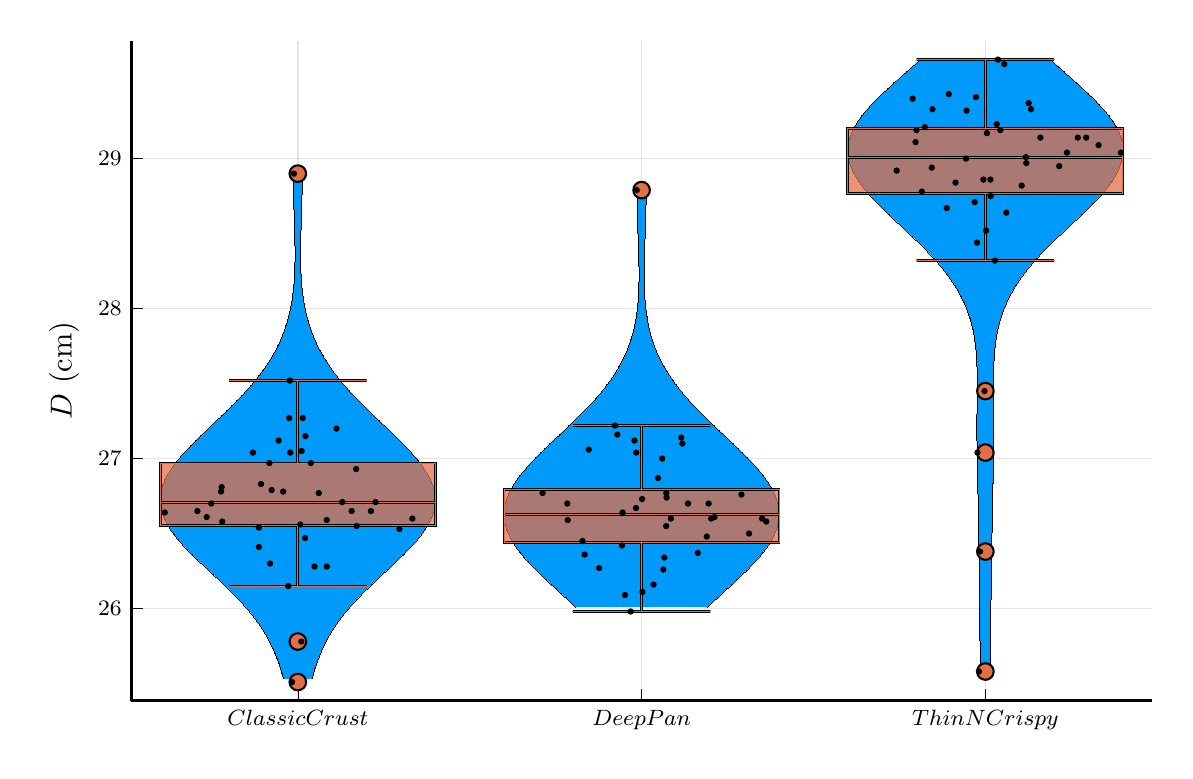
\begin{tikzpicture}[/tikz/background rectangle/.style={fill={rgb,1:red,1.0;green,1.0;blue,1.0}, draw opacity={1.0}}, show background rectangle]
\begin{axis}[point meta max={nan}, point meta min={nan}, legend cell align={left}, legend columns={1}, title={}, title style={at={{(0.5,1)}}, anchor={south}, font={{\fontsize{14 pt}{18.2 pt}\selectfont}}, color={rgb,1:red,0.0;green,0.0;blue,0.0}, draw opacity={1.0}, rotate={0.0}}, legend style={color={rgb,1:red,0.0;green,0.0;blue,0.0}, draw opacity={1.0}, line width={1}, solid, fill={rgb,1:red,1.0;green,1.0;blue,1.0}, fill opacity={1.0}, text opacity={1.0}, font={{\fontsize{8 pt}{10.4 pt}\selectfont}}, text={rgb,1:red,0.0;green,0.0;blue,0.0}, cells={anchor={center}}, at={(1.02, 1)}, anchor={north west}}, axis background/.style={fill={rgb,1:red,1.0;green,1.0;blue,1.0}, opacity={1.0}}, anchor={north west}, xshift={1.0mm}, yshift={-1.0mm}, width={145.4mm}, height={99.6mm}, scaled x ticks={false}, xlabel={}, x tick style={color={rgb,1:red,0.0;green,0.0;blue,0.0}, opacity={1.0}}, x tick label style={color={rgb,1:red,0.0;green,0.0;blue,0.0}, opacity={1.0}, rotate={0}}, xlabel style={at={(ticklabel cs:0.5)}, anchor=near ticklabel, at={{(ticklabel cs:0.5)}}, anchor={near ticklabel}, font={{\fontsize{11 pt}{14.3 pt}\selectfont}}, color={rgb,1:red,0.0;green,0.0;blue,0.0}, draw opacity={1.0}, rotate={0.0}}, xmajorgrids={true}, xmin={0.015999999999999986}, xmax={2.984}, xtick={{0.5,1.5,2.5}}, xticklabels={{$ClassicCrust$,$DeepPan$,$ThinNCrispy$}}, xtick align={inside}, xticklabel style={font={{\fontsize{8 pt}{10.4 pt}\selectfont}}, color={rgb,1:red,0.0;green,0.0;blue,0.0}, draw opacity={1.0}, rotate={0.0}}, x grid style={color={rgb,1:red,0.0;green,0.0;blue,0.0}, draw opacity={0.1}, line width={0.5}, solid}, axis x line*={left}, x axis line style={color={rgb,1:red,0.0;green,0.0;blue,0.0}, draw opacity={1.0}, line width={1}, solid}, scaled y ticks={false}, ylabel={$D \text{ (cm)}$}, y tick style={color={rgb,1:red,0.0;green,0.0;blue,0.0}, opacity={1.0}}, y tick label style={color={rgb,1:red,0.0;green,0.0;blue,0.0}, opacity={1.0}, rotate={0}}, ylabel style={at={(ticklabel cs:0.5)}, anchor=near ticklabel, at={{(ticklabel cs:0.5)}}, anchor={near ticklabel}, font={{\fontsize{11 pt}{14.3 pt}\selectfont}}, color={rgb,1:red,0.0;green,0.0;blue,0.0}, draw opacity={1.0}, rotate={0.0}}, ymajorgrids={true}, ymin={25.3855}, ymax={29.7845}, ytick={{26.0,27.0,28.0,29.0}}, yticklabels={{$26$,$27$,$28$,$29$}}, ytick align={inside}, yticklabel style={font={{\fontsize{8 pt}{10.4 pt}\selectfont}}, color={rgb,1:red,0.0;green,0.0;blue,0.0}, draw opacity={1.0}, rotate={0.0}}, y grid style={color={rgb,1:red,0.0;green,0.0;blue,0.0}, draw opacity={0.1}, line width={0.5}, solid}, axis y line*={left}, y axis line style={color={rgb,1:red,0.0;green,0.0;blue,0.0}, draw opacity={1.0}, line width={1}, solid}, colorbar={false}]
    \addplot[color={rgb,1:red,0.0;green,0.0;blue,0.0}, name path={a5401ee7-c9bd-49a6-bda9-2f0aa51e70d0}, area legend, fill={rgb,1:red,0.0;green,0.6056;blue,0.9787}, fill opacity={1.0}, draw opacity={1.0}, line width={0}, solid, forget plot]
        table[row sep={\\}]
        {
            \\
            0.5416546719989935  25.531462365003275  \\
            0.5455173663675735  25.56460172411212  \\
            0.5497551916834748  25.597741083220967  \\
            0.554412686311593  25.63088044232981  \\
            0.5595366692876907  25.66401980143866  \\
            0.5651752525512741  25.697159160547503  \\
            0.5713766358438511  25.73029851965635  \\
            0.5781876981586067  25.763437878765195  \\
            0.5856524094912091  25.796577237874043  \\
            0.5938100966687482  25.829716596982887  \\
            0.6026936068103179  25.862855956091735  \\
            0.6123274210459336  25.89599531520058  \\
            0.6227257790143134  25.929134674309427  \\
            0.6338908808936161  25.96227403341827  \\
            0.6458112378289083  25.99541339252712  \\
            0.6584602431853142  26.028552751635964  \\
            0.6717950357270042  26.06169211074481  \\
            0.6857557213504658  26.094831469853656  \\
            0.700265012266001  26.127970828962503  \\
            0.7152283315587824  26.16111018807135  \\
            0.7305344170787273  26.194249547180195  \\
            0.7460564420004833  26.227388906289043  \\
            0.7616536507389688  26.260528265397888  \\
            0.7771734889511162  26.293667624506735  \\
            0.7924541859927141  26.32680698361558  \\
            0.8073277284237828  26.359946342724427  \\
            0.821623145006784  26.39308570183327  \\
            0.8351700081422369  26.42622506094212  \\
            0.8478020447730197  26.459364420050964  \\
            0.8593607422439833  26.49250377915981  \\
            0.8696988319921148  26.525643138268656  \\
            0.878683536560777  26.558782497377504  \\
            0.8861994732741596  26.591921856486348  \\
            0.8921511206560172  26.625061215595196  \\
            0.8964647707086992  26.65820057470404  \\
            0.8990899105961845  26.691339933812888  \\
            0.8999999999999999  26.724479292921732  \\
            0.8991926342055114  26.75761865203058  \\
            0.8966891065439772  26.790758011139424  \\
            0.8925334059184598  26.82389737024827  \\
            0.8867907046603598  26.857036729357116  \\
            0.8795454079797738  26.890176088465964  \\
            0.8708988481269102  26.923315447574808  \\
            0.8609667137066025  26.956454806683656  \\
            0.8498763073208149  26.9895941657925  \\
            0.8377637230823629  27.022733524901348  \\
            0.8247710300283333  27.055872884010192  \\
            0.8110435387451941  27.08901224311904  \\
            0.7967272174142834  27.122151602227884  \\
            0.781966310873251  27.155290961336732  \\
            0.7669012030347919  27.188430320445576  \\
            0.7516665499063935  27.221569679554424  \\
            0.7363896981901761  27.254709038663268  \\
            0.7211893935308433  27.287848397772116  \\
            0.7061747732695997  27.32098775688096  \\
            0.6914446312263945  27.354127115989808  \\
            0.6770869365864118  27.387266475098652  \\
            0.6631785852904625  27.4204058342075  \\
            0.6497853602042466  27.453545193316344  \\
            0.6369620754870208  27.486684552425192  \\
            0.6247528806883456  27.519823911534036  \\
            0.6131917008706249  27.552963270642884  \\
            0.6023027902152646  27.58610262975173  \\
            0.5921013779014835  27.619241988860576  \\
            0.5825943863886437  27.65238134796942  \\
            0.5737812034863905  27.68552070707827  \\
            0.565654490719729  27.718660066187113  \\
            0.5582010114936977  27.75179942529596  \\
            0.5514024634750039  27.784938784404805  \\
            0.5452363004980496  27.818078143513652  \\
            0.5396765302412433  27.851217502622497  \\
            0.5346944749748516  27.884356861731344  \\
            0.530259483910987  27.91749622084019  \\
            0.5263395871290542  27.950635579949036  \\
            0.5229020827242443  27.98377493905788  \\
            0.5199140507281703  28.01691429816673  \\
            0.5173427894533115  28.050053657275573  \\
            0.515156172170696  28.08319301638442  \\
            0.5133229243804411  28.116332375493265  \\
            0.5118128243014225  28.149471734602113  \\
            0.5105968315040759  28.182611093710957  \\
            0.5096471507484922  28.215750452819805  \\
            0.508937239976927  28.24888981192865  \\
            0.5084417729575129  28.282029171037497  \\
            0.5081365682045261  28.315168530146344  \\
            0.5079984964433059  28.34830788925519  \\
            0.5080053789961653  28.381447248364037  \\
            0.5081358890131784  28.41458660747288  \\
            0.5083694664588743  28.44772596658173  \\
            0.5086862562221849  28.480865325690573  \\
            0.5090670767026144  28.51400468479942  \\
            0.5094934238306321  28.547144043908265  \\
            0.5099475128219763  28.580283403017113  \\
            0.5104123571831332  28.613422762125957  \\
            0.510871881732695  28.646562121234805  \\
            0.511311063840124  28.67970148034365  \\
            0.5117160948643865  28.712840839452497  \\
            0.5120745520389981  28.74598019856134  \\
            0.5123755699101592  28.77911955767019  \\
            0.51260999996853  28.812258916779033  \\
            0.5127705473583969  28.84539827588788  \\
            0.5128518744901073  28.878537634996725  \\
            0.4871481255098928  28.878537634996725  \\
            0.48722945264160317  28.84539827588788  \\
            0.48739000003147004  28.812258916779033  \\
            0.48762443008984085  28.77911955767019  \\
            0.48792544796100196  28.74598019856134  \\
            0.4882839051356135  28.712840839452497  \\
            0.48868893615987596  28.67970148034365  \\
            0.48912811826730496  28.646562121234805  \\
            0.48958764281686684  28.613422762125957  \\
            0.49005248717802374  28.580283403017113  \\
            0.4905065761693678  28.547144043908265  \\
            0.49093292329738564  28.51400468479942  \\
            0.49131374377781517  28.480865325690573  \\
            0.4916305335411258  28.44772596658173  \\
            0.4918641109868216  28.41458660747288  \\
            0.49199462100383473  28.381447248364037  \\
            0.49200150355669414  28.34830788925519  \\
            0.49186343179547387  28.315168530146344  \\
            0.4915582270424871  28.282029171037497  \\
            0.49106276002307303  28.24888981192865  \\
            0.49035284925150774  28.215750452819805  \\
            0.48940316849592413  28.182611093710957  \\
            0.4881871756985775  28.149471734602113  \\
            0.48667707561955886  28.116332375493265  \\
            0.48484382782930396  28.08319301638442  \\
            0.48265721054668853  28.050053657275573  \\
            0.4800859492718296  28.01691429816673  \\
            0.47709791727575573  27.98377493905788  \\
            0.4736604128709459  27.950635579949036  \\
            0.469740516089013  27.91749622084019  \\
            0.46530552502514844  27.884356861731344  \\
            0.46032346975875676  27.851217502622497  \\
            0.45476369950195045  27.818078143513652  \\
            0.4485975365249962  27.784938784404805  \\
            0.4417989885063022  27.75179942529596  \\
            0.43434550928027105  27.718660066187113  \\
            0.4262187965136095  27.68552070707827  \\
            0.41740561361135636  27.65238134796942  \\
            0.40789862209851646  27.619241988860576  \\
            0.39769720978473544  27.58610262975173  \\
            0.38680829912937514  27.552963270642884  \\
            0.3752471193116544  27.519823911534036  \\
            0.3630379245129792  27.486684552425192  \\
            0.3502146397957534  27.453545193316344  \\
            0.3368214147095375  27.4204058342075  \\
            0.3229130634135881  27.387266475098652  \\
            0.30855536877360545  27.354127115989808  \\
            0.29382522673040035  27.32098775688096  \\
            0.2788106064691567  27.287848397772116  \\
            0.26361030180982387  27.254709038663268  \\
            0.24833345009360647  27.221569679554424  \\
            0.23309879696520802  27.188430320445576  \\
            0.21803368912674903  27.155290961336732  \\
            0.20327278258571652  27.122151602227884  \\
            0.18895646125480592  27.08901224311904  \\
            0.1752289699716667  27.055872884010192  \\
            0.16223627691763715  27.022733524901348  \\
            0.15012369267918518  26.9895941657925  \\
            0.1390332862933975  26.956454806683656  \\
            0.12910115187308985  26.923315447574808  \\
            0.12045459202022624  26.890176088465964  \\
            0.11320929533964025  26.857036729357116  \\
            0.10746659408154019  26.82389737024827  \\
            0.10331089345602285  26.790758011139424  \\
            0.10080736579448857  26.75761865203058  \\
            0.10000000000000003  26.724479292921732  \\
            0.10091008940381552  26.691339933812888  \\
            0.10353522929130082  26.65820057470404  \\
            0.1078488793439828  26.625061215595196  \\
            0.11380052672584035  26.591921856486348  \\
            0.12131646343922292  26.558782497377504  \\
            0.13030116800788522  26.525643138268656  \\
            0.14063925775601677  26.49250377915981  \\
            0.15219795522698026  26.459364420050964  \\
            0.1648299918577632  26.42622506094212  \\
            0.17837685499321598  26.39308570183327  \\
            0.1926722715762173  26.359946342724427  \\
            0.20754581400728594  26.32680698361558  \\
            0.22282651104888385  26.293667624506735  \\
            0.2383463492610311  26.260528265397888  \\
            0.25394355799951673  26.227388906289043  \\
            0.26946558292127265  26.194249547180195  \\
            0.2847716684412176  26.16111018807135  \\
            0.299734987733999  26.127970828962503  \\
            0.3142442786495342  26.094831469853656  \\
            0.32820496427299584  26.06169211074481  \\
            0.3415397568146859  26.028552751635964  \\
            0.35418876217109174  25.99541339252712  \\
            0.3661091191063839  25.96227403341827  \\
            0.3772742209856866  25.929134674309427  \\
            0.3876725789540664  25.89599531520058  \\
            0.3973063931896821  25.862855956091735  \\
            0.4061899033312518  25.829716596982887  \\
            0.4143475905087909  25.796577237874043  \\
            0.4218123018413933  25.763437878765195  \\
            0.4286233641561489  25.73029851965635  \\
            0.43482474744872596  25.697159160547503  \\
            0.44046333071230925  25.66401980143866  \\
            0.44558731368840704  25.63088044232981  \\
            0.4502448083165252  25.597741083220967  \\
            0.45448263363242647  25.56460172411212  \\
            0.45834532800100647  25.531462365003275  \\
        }
        ;
    \addplot[color={rgb,1:red,0.0;green,0.0;blue,0.0}, name path={a5401ee7-c9bd-49a6-bda9-2f0aa51e70d0}, area legend, fill={rgb,1:red,0.0;green,0.6056;blue,0.9787}, fill opacity={1.0}, draw opacity={1.0}, line width={0}, solid, forget plot]
        table[row sep={\\}]
        {
            \\
            1.6915428167553113  26.009772225874137  \\
            1.705498167548933  26.03999701211866  \\
            1.7196833257118687  26.070221798363185  \\
            1.734012455265582  26.10044658460771  \\
            1.7483924708758605  26.130671370852234  \\
            1.7627238724554946  26.160896157096758  \\
            1.776901759669559  26.191120943341286  \\
            1.7908170184963537  26.22134572958581  \\
            1.8043576661437453  26.251570515830334  \\
            1.8174103345709458  26.28179530207486  \\
            1.829861866886437  26.312020088319382  \\
            1.841600995283435  26.342244874563907  \\
            1.8525200642503874  26.37246966080843  \\
            1.8625167588667153  26.402694447052955  \\
            1.8714957953481965  26.43291923329748  \\
            1.8793705298784449  26.463144019542003  \\
            1.886064442320066  26.493368805786528  \\
            1.891512453722461  26.52359359203105  \\
            1.895662040616127  26.553818378275576  \\
            1.8984741147858957  26.584043164520104  \\
            1.8999236443273053  26.614267950764628  \\
            1.9  26.644492737009152  \\
            1.8987070198149343  26.674717523253676  \\
            1.8960627939936465  26.7049423094982  \\
            1.8920991814612191  26.735167095742725  \\
            1.8868610774314865  26.76539188198725  \\
            1.8804054590036947  26.795616668231773  \\
            1.8728002416706562  26.825841454476297  \\
            1.864122983984835  26.85606624072082  \\
            1.854459480191403  26.886291026965345  \\
            1.843902281379754  26.91651581320987  \\
            1.8325491847034072  26.946740599454394  \\
            1.8205017276519053  26.976965385698918  \\
            1.807863720492794  27.007190171943446  \\
            1.7947398451658412  27.03741495818797  \\
            1.781234343470441  27.067639744432494  \\
            1.7674498117134019  27.09786453067702  \\
            1.7534861134306685  27.128089316921542  \\
            1.7394394166708156  27.158314103166067  \\
            1.7254013578738587  27.18853888941059  \\
            1.711458330762055  27.218763675655115  \\
            1.6976908959626256  27.24898846189964  \\
            1.6841733053066084  27.279213248144163  \\
            1.6709731338205303  27.309438034388688  \\
            1.6581510122156051  27.33966282063321  \\
            1.6457604530078398  27.369887606877736  \\
            1.6338477640745004  27.400112393122264  \\
            1.6224520442682193  27.430337179366788  \\
            1.611605256486098  27.460561965611312  \\
            1.6013323741752068  27.490786751855836  \\
            1.5916515975382532  27.52101153810036  \\
            1.5825746356228447  27.551236324344885  \\
            1.5741070500237577  27.58146111058941  \\
            1.5662486551357035  27.611685896833933  \\
            1.5589939688393597  27.641910683078457  \\
            1.552332706290441  27.67213546932298  \\
            1.5462503082321148  27.702360255567505  \\
            1.5407284940921124  27.73258504181203  \\
            1.5357458291776003  27.762809828056554  \\
            1.5312782946465666  27.79303461430108  \\
            1.52729984869267  27.823259400545606  \\
            1.5237829675796275  27.85348418679013  \\
            1.520699155817458  27.883708973034654  \\
            1.5180194158703328  27.91393375927918  \\
            1.5157146692792582  27.944158545523702  \\
            1.5137561229025525  27.974383331768227  \\
            1.5121155760345495  28.00460811801275  \\
            1.5107656663576023  28.034832904257275  \\
            1.5096800549084288  28.0650576905018  \\
            1.5088335523924954  28.095282476746323  \\
            1.508202191161741  28.125507262990848  \\
            1.5077632488955663  28.15573204923537  \\
            1.5074952314220842  28.185956835479896  \\
            1.5073778231336263  28.216181621724424  \\
            1.5073918140543683  28.246406407968948  \\
            1.5075190127955644  28.276631194213472  \\
            1.5077421543917786  28.306855980457996  \\
            1.5080448113745786  28.33708076670252  \\
            1.508411315450147  28.367305552947045  \\
            1.5088266958602699  28.39753033919157  \\
            1.5092766389901486  28.427755125436093  \\
            1.5097474721181374  28.457979911680617  \\
            1.5102261724639152  28.48820469792514  \\
            1.5107004009667047  28.518429484169665  \\
            1.511158558596067  28.54865427041419  \\
            1.5115898615411043  28.578879056658714  \\
            1.5119844304071217  28.60910384290324  \\
            1.5123333876271343  28.639328629147766  \\
            1.512628956709176  28.66955341539229  \\
            1.5128645567121464  28.699778201636814  \\
            1.513034885477437  28.73000298788134  \\
            1.5131359856266164  28.760227774125863  \\
            1.4868640143733836  28.760227774125863  \\
            1.486965114522563  28.73000298788134  \\
            1.4871354432878536  28.699778201636814  \\
            1.487371043290824  28.66955341539229  \\
            1.4876666123728657  28.639328629147766  \\
            1.4880155695928783  28.60910384290324  \\
            1.4884101384588957  28.578879056658714  \\
            1.488841441403933  28.54865427041419  \\
            1.4892995990332953  28.518429484169665  \\
            1.4897738275360848  28.48820469792514  \\
            1.4902525278818626  28.457979911680617  \\
            1.4907233610098514  28.427755125436093  \\
            1.4911733041397301  28.39753033919157  \\
            1.491588684549853  28.367305552947045  \\
            1.4919551886254214  28.33708076670252  \\
            1.4922578456082214  28.306855980457996  \\
            1.4924809872044356  28.276631194213472  \\
            1.4926081859456317  28.246406407968948  \\
            1.4926221768663737  28.216181621724424  \\
            1.4925047685779158  28.185956835479896  \\
            1.4922367511044337  28.15573204923537  \\
            1.491797808838259  28.125507262990848  \\
            1.4911664476075046  28.095282476746323  \\
            1.4903199450915712  28.0650576905018  \\
            1.4892343336423977  28.034832904257275  \\
            1.4878844239654505  28.00460811801275  \\
            1.4862438770974475  27.974383331768227  \\
            1.4842853307207418  27.944158545523702  \\
            1.4819805841296672  27.91393375927918  \\
            1.479300844182542  27.883708973034654  \\
            1.4762170324203725  27.85348418679013  \\
            1.47270015130733  27.823259400545606  \\
            1.4687217053534334  27.79303461430108  \\
            1.4642541708223997  27.762809828056554  \\
            1.4592715059078876  27.73258504181203  \\
            1.4537496917678852  27.702360255567505  \\
            1.447667293709559  27.67213546932298  \\
            1.4410060311606403  27.641910683078457  \\
            1.4337513448642965  27.611685896833933  \\
            1.4258929499762423  27.58146111058941  \\
            1.4174253643771553  27.551236324344885  \\
            1.4083484024617468  27.52101153810036  \\
            1.3986676258247932  27.490786751855836  \\
            1.388394743513902  27.460561965611312  \\
            1.3775479557317807  27.430337179366788  \\
            1.3661522359254996  27.400112393122264  \\
            1.3542395469921602  27.369887606877736  \\
            1.3418489877843949  27.33966282063321  \\
            1.3290268661794697  27.309438034388688  \\
            1.3158266946933916  27.279213248144163  \\
            1.3023091040373744  27.24898846189964  \\
            1.288541669237945  27.218763675655115  \\
            1.2745986421261413  27.18853888941059  \\
            1.2605605833291844  27.158314103166067  \\
            1.2465138865693315  27.128089316921542  \\
            1.2325501882865981  27.09786453067702  \\
            1.218765656529559  27.067639744432494  \\
            1.2052601548341588  27.03741495818797  \\
            1.192136279507206  27.007190171943446  \\
            1.1794982723480947  26.976965385698918  \\
            1.1674508152965928  26.946740599454394  \\
            1.156097718620246  26.91651581320987  \\
            1.145540519808597  26.886291026965345  \\
            1.135877016015165  26.85606624072082  \\
            1.1271997583293438  26.825841454476297  \\
            1.1195945409963053  26.795616668231773  \\
            1.1131389225685135  26.76539188198725  \\
            1.1079008185387809  26.735167095742725  \\
            1.1039372060063535  26.7049423094982  \\
            1.1012929801850657  26.674717523253676  \\
            1.1  26.644492737009152  \\
            1.1000763556726947  26.614267950764628  \\
            1.1015258852141043  26.584043164520104  \\
            1.104337959383873  26.553818378275576  \\
            1.108487546277539  26.52359359203105  \\
            1.113935557679934  26.493368805786528  \\
            1.1206294701215551  26.463144019542003  \\
            1.1285042046518035  26.43291923329748  \\
            1.1374832411332847  26.402694447052955  \\
            1.1474799357496126  26.37246966080843  \\
            1.158399004716565  26.342244874563907  \\
            1.170138133113563  26.312020088319382  \\
            1.1825896654290542  26.28179530207486  \\
            1.1956423338562547  26.251570515830334  \\
            1.2091829815036463  26.22134572958581  \\
            1.223098240330441  26.191120943341286  \\
            1.2372761275445054  26.160896157096758  \\
            1.2516075291241395  26.130671370852234  \\
            1.265987544734418  26.10044658460771  \\
            1.2803166742881313  26.070221798363185  \\
            1.294501832451067  26.03999701211866  \\
            1.3084571832446887  26.009772225874137  \\
        }
        ;
    \addplot[color={rgb,1:red,0.0;green,0.0;blue,0.0}, name path={a5401ee7-c9bd-49a6-bda9-2f0aa51e70d0}, area legend, fill={rgb,1:red,0.0;green,0.6056;blue,0.9787}, fill opacity={1.0}, draw opacity={1.0}, line width={0}, solid, forget plot]
        table[row sep={\\}]
        {
            \\
            2.514720051351438  25.588328383529394  \\
            2.515002317012145  25.624935079321656  \\
            2.5152282860158723  25.66154177511392  \\
            2.5154044567319644  25.698148470906183  \\
            2.5155388447897264  25.734755166698445  \\
            2.5156405455746005  25.77136186249071  \\
            2.5157192436595786  25.807968558282973  \\
            2.5157847006379734  25.844575254075234  \\
            2.5158462547598424  25.8811819498675  \\
            2.515912365202925  25.917788645659762  \\
            2.515990230708793  25.954395341452024  \\
            2.5160855068796733  25.99100203724429  \\
            2.5162021390584126  26.02760873303655  \\
            2.516342318974277  26.064215428828813  \\
            2.5165065639285804  26.10082212462108  \\
            2.5166939079818667  26.13742882041334  \\
            2.5169021861546708  26.174035516205606  \\
            2.5171283857656834  26.210642211997868  \\
            2.5173690342733894  26.24724890779013  \\
            2.5176205907474727  26.283855603582396  \\
            2.5178798085452168  26.320462299374658  \\
            2.5181440398444908  26.35706899516692  \\
            2.518411458101539  26.393675690959185  \\
            2.518681181773073  26.430282386751447  \\
            2.5189532911300287  26.46688908254371  \\
            2.5192287389644608  26.503495778335974  \\
            2.5195091646969914  26.540102474128236  \\
            2.519796629121278  26.5767091699205  \\
            2.5200932931746505  26.613315865712764  \\
            2.5204010682618834  26.649922561505026  \\
            2.520721267538528  26.686529257297288  \\
            2.5210542871464754  26.723135953089553  \\
            2.521399343853436  26.759742648881815  \\
            2.5217542912187105  26.796349344674077  \\
            2.5221155307581133  26.832956040466343  \\
            2.52247802815388  26.869562736258604  \\
            2.522835437909576  26.906169432050866  \\
            2.5231803335045564  26.942776127843132  \\
            2.523504534489946  26.979382823635394  \\
            2.523799517401544  27.015989519427656  \\
            2.524056894021474  27.05259621521992  \\
            2.5242689384415007  27.089202911012183  \\
            2.524429143488973  27.125809606804445  \\
            2.524532787202512  27.16241630259671  \\
            2.52457749096368  27.199022998388973  \\
            2.5245637523587434  27.235629694181235  \\
            2.5244954376308035  27.2722363899735  \\
            2.5243802204964894  27.308843085765762  \\
            2.5242299560072388  27.345449781558024  \\
            2.5240609799558764  27.38205647735029  \\
            2.523894326039854  27.41866317314255  \\
            2.5237558546055188  27.455269868934813  \\
            2.5236762883437773  27.49187656472708  \\
            2.5236911518152234  27.52848326051934  \\
            2.5238406131624114  27.565089956311603  \\
            2.5241692277994194  27.60169665210387  \\
            2.524725585203409  27.63830334789613  \\
            2.5255618610930184  27.674910043688396  \\
            2.526733278175488  27.711516739480658  \\
            2.5282974791965227  27.74812343527292  \\
            2.5303138161806884  27.784730131065185  \\
            2.532842559500717  27.821336826857447  \\
            2.5359440298214033  27.85794352264971  \\
            2.5396776551607583  27.894550218441974  \\
            2.5441009545028135  27.931156914234236  \\
            2.5492684488487454  27.9677636100265  \\
            2.555230500610338  28.004370305818764  \\
            2.562032083145247  28.040977001611026  \\
            2.5697114842915547  28.077583697403288  \\
            2.578298951196249  28.114190393195553  \\
            2.5878152886586467  28.150797088987815  \\
            2.5982704295962837  28.187403784780077  \\
            2.6096620038956355  28.224010480572343  \\
            2.6219739404683278  28.260617176364605  \\
            2.6351751462627133  28.297223872156867  \\
            2.649218314602457  28.333830567949132  \\
            2.664038922753004  28.370437263741394  \\
            2.679554484215044  28.407043959533656  \\
            2.6956641240849684  28.44365065532592  \\
            2.7122485451630958  28.480257351118183  \\
            2.7291704477448624  28.516864046910445  \\
            2.746275456835504  28.55347074270271  \\
            2.7633935968010674  28.590077438494973  \\
            2.780341335440189  28.626684134287235  \\
            2.7969241976958754  28.6632908300795  \\
            2.8129399246100424  28.699897525871762  \\
            2.8281821268269463  28.736504221664024  \\
            2.842444355371039  28.77311091745629  \\
            2.8555244870990966  28.80971761324855  \\
            2.8672292997394724  28.846324309040813  \\
            2.8773790933042536  28.88293100483308  \\
            2.8858122022432227  28.91953770062534  \\
            2.89238923707929  28.956144396417603  \\
            2.8969968961413675  28.99275109220987  \\
            2.899551197685561  29.02935778800213  \\
            2.9  29.065964483794392  \\
            2.898324701384803  29.102571179586658  \\
            2.89454104210651  29.13917787537892  \\
            2.8886989650815402  29.175784571171185  \\
            2.8808815293836516  29.212391266963447  \\
            2.8712029087452424  29.24899796275571  \\
            2.8598055440162713  29.285604658547975  \\
            2.8468565521081977  29.322211354340237  \\
            2.8325435225269056  29.3588180501325  \\
            2.817069854737451  29.395424745924764  \\
            2.800649804252033  29.432031441717026  \\
            2.7835034118984465  29.468638137509288  \\
            2.765851489106506  29.505244833301553  \\
            2.7479108226241045  29.541851529093815  \\
            2.729889745663801  29.578458224886077  \\
            2.7119842002760937  29.615064920678343  \\
            2.6943743892126615  29.651671616470605  \\
            2.3056256107873385  29.651671616470605  \\
            2.2880157997239063  29.615064920678343  \\
            2.270110254336199  29.578458224886077  \\
            2.2520891773758955  29.541851529093815  \\
            2.234148510893494  29.505244833301553  \\
            2.2164965881015535  29.468638137509288  \\
            2.199350195747967  29.432031441717026  \\
            2.182930145262549  29.395424745924764  \\
            2.1674564774730944  29.3588180501325  \\
            2.1531434478918023  29.322211354340237  \\
            2.1401944559837287  29.285604658547975  \\
            2.1287970912547576  29.24899796275571  \\
            2.1191184706163484  29.212391266963447  \\
            2.1113010349184598  29.175784571171185  \\
            2.10545895789349  29.13917787537892  \\
            2.101675298615197  29.102571179586658  \\
            2.1  29.065964483794392  \\
            2.100448802314439  29.02935778800213  \\
            2.1030031038586325  28.99275109220987  \\
            2.10761076292071  28.956144396417603  \\
            2.1141877977567773  28.91953770062534  \\
            2.1226209066957464  28.88293100483308  \\
            2.1327707002605276  28.846324309040813  \\
            2.1444755129009034  28.80971761324855  \\
            2.157555644628961  28.77311091745629  \\
            2.1718178731730537  28.736504221664024  \\
            2.1870600753899576  28.699897525871762  \\
            2.2030758023041246  28.6632908300795  \\
            2.219658664559811  28.626684134287235  \\
            2.2366064031989326  28.590077438494973  \\
            2.253724543164496  28.55347074270271  \\
            2.2708295522551376  28.516864046910445  \\
            2.2877514548369042  28.480257351118183  \\
            2.3043358759150316  28.44365065532592  \\
            2.320445515784956  28.407043959533656  \\
            2.335961077246996  28.370437263741394  \\
            2.350781685397543  28.333830567949132  \\
            2.3648248537372867  28.297223872156867  \\
            2.3780260595316722  28.260617176364605  \\
            2.3903379961043645  28.224010480572343  \\
            2.4017295704037163  28.187403784780077  \\
            2.4121847113413533  28.150797088987815  \\
            2.421701048803751  28.114190393195553  \\
            2.4302885157084453  28.077583697403288  \\
            2.437967916854753  28.040977001611026  \\
            2.444769499389662  28.004370305818764  \\
            2.4507315511512546  27.9677636100265  \\
            2.4558990454971865  27.931156914234236  \\
            2.4603223448392417  27.894550218441974  \\
            2.4640559701785967  27.85794352264971  \\
            2.467157440499283  27.821336826857447  \\
            2.4696861838193116  27.784730131065185  \\
            2.4717025208034773  27.74812343527292  \\
            2.473266721824512  27.711516739480658  \\
            2.4744381389069816  27.674910043688396  \\
            2.475274414796591  27.63830334789613  \\
            2.4758307722005806  27.60169665210387  \\
            2.4761593868375886  27.565089956311603  \\
            2.4763088481847766  27.52848326051934  \\
            2.4763237116562227  27.49187656472708  \\
            2.4762441453944812  27.455269868934813  \\
            2.476105673960146  27.41866317314255  \\
            2.4759390200441236  27.38205647735029  \\
            2.4757700439927612  27.345449781558024  \\
            2.4756197795035106  27.308843085765762  \\
            2.4755045623691965  27.2722363899735  \\
            2.4754362476412566  27.235629694181235  \\
            2.47542250903632  27.199022998388973  \\
            2.475467212797488  27.16241630259671  \\
            2.475570856511027  27.125809606804445  \\
            2.4757310615584993  27.089202911012183  \\
            2.475943105978526  27.05259621521992  \\
            2.476200482598456  27.015989519427656  \\
            2.476495465510054  26.979382823635394  \\
            2.4768196664954436  26.942776127843132  \\
            2.477164562090424  26.906169432050866  \\
            2.47752197184612  26.869562736258604  \\
            2.4778844692418867  26.832956040466343  \\
            2.4782457087812895  26.796349344674077  \\
            2.478600656146564  26.759742648881815  \\
            2.4789457128535246  26.723135953089553  \\
            2.479278732461472  26.686529257297288  \\
            2.4795989317381166  26.649922561505026  \\
            2.4799067068253495  26.613315865712764  \\
            2.480203370878722  26.5767091699205  \\
            2.4804908353030086  26.540102474128236  \\
            2.4807712610355392  26.503495778335974  \\
            2.4810467088699713  26.46688908254371  \\
            2.481318818226927  26.430282386751447  \\
            2.481588541898461  26.393675690959185  \\
            2.4818559601555092  26.35706899516692  \\
            2.4821201914547832  26.320462299374658  \\
            2.4823794092525273  26.283855603582396  \\
            2.4826309657266106  26.24724890779013  \\
            2.4828716142343166  26.210642211997868  \\
            2.4830978138453292  26.174035516205606  \\
            2.4833060920181333  26.13742882041334  \\
            2.4834934360714196  26.10082212462108  \\
            2.483657681025723  26.064215428828813  \\
            2.4837978609415874  26.02760873303655  \\
            2.4839144931203267  25.99100203724429  \\
            2.484009769291207  25.954395341452024  \\
            2.484087634797075  25.917788645659762  \\
            2.4841537452401576  25.8811819498675  \\
            2.4842152993620266  25.844575254075234  \\
            2.4842807563404214  25.807968558282973  \\
            2.4843594544253995  25.77136186249071  \\
            2.4844611552102736  25.734755166698445  \\
            2.4845955432680356  25.698148470906183  \\
            2.4847717139841277  25.66154177511392  \\
            2.484997682987855  25.624935079321656  \\
            2.485279948648562  25.588328383529394  \\
        }
        ;
    \addplot[color={rgb,1:red,0.0;green,0.0;blue,0.0}, name path={dae1bd37-787e-407c-93ca-93e9ee143b1b}, area legend, fill={rgb,1:red,0.8889;green,0.4356;blue,0.2781}, fill opacity={0.75}, draw opacity={1.0}, line width={1}, solid, forget plot]
        table[row sep={\\}]
        {
            \\
            0.5  26.15  \\
            0.3  26.15  \\
            0.7  26.15  \\
            0.5  26.15  \\
            0.5  26.552500000000002  \\
        }
        ;
    \addplot[color={rgb,1:red,0.0;green,0.0;blue,0.0}, name path={dae1bd37-787e-407c-93ca-93e9ee143b1b}, area legend, fill={rgb,1:red,0.8889;green,0.4356;blue,0.2781}, fill opacity={0.75}, draw opacity={1.0}, line width={1}, solid, forget plot]
        table[row sep={\\}]
        {
            \\
            0.9  26.552500000000002  \\
            0.9  26.705  \\
            0.09999999999999998  26.705  \\
            0.09999999999999998  26.552500000000002  \\
            0.9  26.552500000000002  \\
            0.9  26.705  \\
        }
        ;
    \addplot[color={rgb,1:red,0.0;green,0.0;blue,0.0}, name path={dae1bd37-787e-407c-93ca-93e9ee143b1b}, area legend, fill={rgb,1:red,0.8889;green,0.4356;blue,0.2781}, fill opacity={0.75}, draw opacity={1.0}, line width={1}, solid, forget plot]
        table[row sep={\\}]
        {
            \\
            0.9  26.97  \\
            0.09999999999999998  26.97  \\
            0.09999999999999998  26.705  \\
            0.9  26.705  \\
            0.9  26.97  \\
            0.5  26.97  \\
        }
        ;
    \addplot[color={rgb,1:red,0.0;green,0.0;blue,0.0}, name path={dae1bd37-787e-407c-93ca-93e9ee143b1b}, area legend, fill={rgb,1:red,0.8889;green,0.4356;blue,0.2781}, fill opacity={0.75}, draw opacity={1.0}, line width={1}, solid, forget plot]
        table[row sep={\\}]
        {
            \\
            0.5  27.52  \\
            0.3  27.52  \\
            0.7  27.52  \\
            0.5  27.52  \\
            0.5  26.97  \\
        }
        ;
    \addplot[color={rgb,1:red,0.0;green,0.0;blue,0.0}, name path={dae1bd37-787e-407c-93ca-93e9ee143b1b}, area legend, fill={rgb,1:red,0.8889;green,0.4356;blue,0.2781}, fill opacity={0.75}, draw opacity={1.0}, line width={1}, solid, forget plot]
        table[row sep={\\}]
        {
            \\
            1.5  25.98  \\
            1.3  25.98  \\
            1.7  25.98  \\
            1.5  25.98  \\
            1.5  26.4425  \\
        }
        ;
    \addplot[color={rgb,1:red,0.0;green,0.0;blue,0.0}, name path={dae1bd37-787e-407c-93ca-93e9ee143b1b}, area legend, fill={rgb,1:red,0.8889;green,0.4356;blue,0.2781}, fill opacity={0.75}, draw opacity={1.0}, line width={1}, solid, forget plot]
        table[row sep={\\}]
        {
            \\
            1.9  26.4425  \\
            1.9  26.625  \\
            1.1  26.625  \\
            1.1  26.4425  \\
            1.9  26.4425  \\
            1.9  26.625  \\
        }
        ;
    \addplot[color={rgb,1:red,0.0;green,0.0;blue,0.0}, name path={dae1bd37-787e-407c-93ca-93e9ee143b1b}, area legend, fill={rgb,1:red,0.8889;green,0.4356;blue,0.2781}, fill opacity={0.75}, draw opacity={1.0}, line width={1}, solid, forget plot]
        table[row sep={\\}]
        {
            \\
            1.9  26.795  \\
            1.1  26.795  \\
            1.1  26.625  \\
            1.9  26.625  \\
            1.9  26.795  \\
            1.5  26.795  \\
        }
        ;
    \addplot[color={rgb,1:red,0.0;green,0.0;blue,0.0}, name path={dae1bd37-787e-407c-93ca-93e9ee143b1b}, area legend, fill={rgb,1:red,0.8889;green,0.4356;blue,0.2781}, fill opacity={0.75}, draw opacity={1.0}, line width={1}, solid, forget plot]
        table[row sep={\\}]
        {
            \\
            1.5  27.22  \\
            1.3  27.22  \\
            1.7  27.22  \\
            1.5  27.22  \\
            1.5  26.795  \\
        }
        ;
    \addplot[color={rgb,1:red,0.0;green,0.0;blue,0.0}, name path={dae1bd37-787e-407c-93ca-93e9ee143b1b}, area legend, fill={rgb,1:red,0.8889;green,0.4356;blue,0.2781}, fill opacity={0.75}, draw opacity={1.0}, line width={1}, solid, forget plot]
        table[row sep={\\}]
        {
            \\
            2.5  28.32  \\
            2.3  28.32  \\
            2.7  28.32  \\
            2.5  28.32  \\
            2.5  28.765  \\
        }
        ;
    \addplot[color={rgb,1:red,0.0;green,0.0;blue,0.0}, name path={dae1bd37-787e-407c-93ca-93e9ee143b1b}, area legend, fill={rgb,1:red,0.8889;green,0.4356;blue,0.2781}, fill opacity={0.75}, draw opacity={1.0}, line width={1}, solid, forget plot]
        table[row sep={\\}]
        {
            \\
            2.9  28.765  \\
            2.9  29.01  \\
            2.1  29.01  \\
            2.1  28.765  \\
            2.9  28.765  \\
            2.9  29.01  \\
        }
        ;
    \addplot[color={rgb,1:red,0.0;green,0.0;blue,0.0}, name path={dae1bd37-787e-407c-93ca-93e9ee143b1b}, area legend, fill={rgb,1:red,0.8889;green,0.4356;blue,0.2781}, fill opacity={0.75}, draw opacity={1.0}, line width={1}, solid, forget plot]
        table[row sep={\\}]
        {
            \\
            2.9  29.200000000000003  \\
            2.1  29.200000000000003  \\
            2.1  29.01  \\
            2.9  29.01  \\
            2.9  29.200000000000003  \\
            2.5  29.200000000000003  \\
        }
        ;
    \addplot[color={rgb,1:red,0.0;green,0.0;blue,0.0}, name path={dae1bd37-787e-407c-93ca-93e9ee143b1b}, area legend, fill={rgb,1:red,0.8889;green,0.4356;blue,0.2781}, fill opacity={0.75}, draw opacity={1.0}, line width={1}, solid, forget plot]
        table[row sep={\\}]
        {
            \\
            2.5  29.66  \\
            2.3  29.66  \\
            2.7  29.66  \\
            2.5  29.66  \\
            2.5  29.200000000000003  \\
        }
        ;
    \addplot[color={rgb,1:red,0.8889;green,0.4356;blue,0.2781}, name path={b1b2d60e-0433-4b6d-9c2c-09b173bc68b7}, only marks, draw opacity={1.0}, line width={0}, solid, mark={*}, mark size={3.0 pt}, mark repeat={1}, mark options={color={rgb,1:red,0.0;green,0.0;blue,0.0}, draw opacity={1.0}, fill={rgb,1:red,0.8889;green,0.4356;blue,0.2781}, fill opacity={1.0}, line width={0.75}, rotate={0}, solid}, forget plot]
        table[row sep={\\}]
        {
            \\
            0.5  25.51  \\
            0.5  28.9  \\
            0.5  25.78  \\
            1.5  28.79  \\
            2.5  27.45  \\
            2.5  26.38  \\
            2.5  27.04  \\
            2.5  25.58  \\
        }
        ;
    \addplot[color={rgb,1:red,0.8889;green,0.4356;blue,0.2781}, name path={0ad018e2-ab23-439c-b10c-ba13eba224af}, draw opacity={1.0}, line width={0}, solid, forget plot]
        table[row sep={\\}]
        {
            \\
            0.5  26.15  \\
            0.3  26.15  \\
            0.7  26.15  \\
            0.5  26.15  \\
            0.5  26.552500000000002  \\
        }
        ;
    \addplot[color={rgb,1:red,0.8889;green,0.4356;blue,0.2781}, name path={0ad018e2-ab23-439c-b10c-ba13eba224af}, draw opacity={1.0}, line width={0}, solid, forget plot]
        table[row sep={\\}]
        {
            \\
            0.9  26.552500000000002  \\
            0.9  26.705  \\
            0.09999999999999998  26.705  \\
            0.09999999999999998  26.552500000000002  \\
            0.9  26.552500000000002  \\
            0.9  26.705  \\
        }
        ;
    \addplot[color={rgb,1:red,0.8889;green,0.4356;blue,0.2781}, name path={0ad018e2-ab23-439c-b10c-ba13eba224af}, draw opacity={1.0}, line width={0}, solid, forget plot]
        table[row sep={\\}]
        {
            \\
            0.9  26.97  \\
            0.09999999999999998  26.97  \\
            0.09999999999999998  26.705  \\
            0.9  26.705  \\
            0.9  26.97  \\
            0.5  26.97  \\
        }
        ;
    \addplot[color={rgb,1:red,0.8889;green,0.4356;blue,0.2781}, name path={0ad018e2-ab23-439c-b10c-ba13eba224af}, draw opacity={1.0}, line width={0}, solid, forget plot]
        table[row sep={\\}]
        {
            \\
            0.5  27.52  \\
            0.3  27.52  \\
            0.7  27.52  \\
            0.5  27.52  \\
            0.5  26.97  \\
        }
        ;
    \addplot[color={rgb,1:red,0.8889;green,0.4356;blue,0.2781}, name path={0ad018e2-ab23-439c-b10c-ba13eba224af}, draw opacity={1.0}, line width={0}, solid, forget plot]
        table[row sep={\\}]
        {
            \\
            1.5  25.98  \\
            1.3  25.98  \\
            1.7  25.98  \\
            1.5  25.98  \\
            1.5  26.4425  \\
        }
        ;
    \addplot[color={rgb,1:red,0.8889;green,0.4356;blue,0.2781}, name path={0ad018e2-ab23-439c-b10c-ba13eba224af}, draw opacity={1.0}, line width={0}, solid, forget plot]
        table[row sep={\\}]
        {
            \\
            1.9  26.4425  \\
            1.9  26.625  \\
            1.1  26.625  \\
            1.1  26.4425  \\
            1.9  26.4425  \\
            1.9  26.625  \\
        }
        ;
    \addplot[color={rgb,1:red,0.8889;green,0.4356;blue,0.2781}, name path={0ad018e2-ab23-439c-b10c-ba13eba224af}, draw opacity={1.0}, line width={0}, solid, forget plot]
        table[row sep={\\}]
        {
            \\
            1.9  26.795  \\
            1.1  26.795  \\
            1.1  26.625  \\
            1.9  26.625  \\
            1.9  26.795  \\
            1.5  26.795  \\
        }
        ;
    \addplot[color={rgb,1:red,0.8889;green,0.4356;blue,0.2781}, name path={0ad018e2-ab23-439c-b10c-ba13eba224af}, draw opacity={1.0}, line width={0}, solid, forget plot]
        table[row sep={\\}]
        {
            \\
            1.5  27.22  \\
            1.3  27.22  \\
            1.7  27.22  \\
            1.5  27.22  \\
            1.5  26.795  \\
        }
        ;
    \addplot[color={rgb,1:red,0.8889;green,0.4356;blue,0.2781}, name path={0ad018e2-ab23-439c-b10c-ba13eba224af}, draw opacity={1.0}, line width={0}, solid, forget plot]
        table[row sep={\\}]
        {
            \\
            2.5  28.32  \\
            2.3  28.32  \\
            2.7  28.32  \\
            2.5  28.32  \\
            2.5  28.765  \\
        }
        ;
    \addplot[color={rgb,1:red,0.8889;green,0.4356;blue,0.2781}, name path={0ad018e2-ab23-439c-b10c-ba13eba224af}, draw opacity={1.0}, line width={0}, solid, forget plot]
        table[row sep={\\}]
        {
            \\
            2.9  28.765  \\
            2.9  29.01  \\
            2.1  29.01  \\
            2.1  28.765  \\
            2.9  28.765  \\
            2.9  29.01  \\
        }
        ;
    \addplot[color={rgb,1:red,0.8889;green,0.4356;blue,0.2781}, name path={0ad018e2-ab23-439c-b10c-ba13eba224af}, draw opacity={1.0}, line width={0}, solid, forget plot]
        table[row sep={\\}]
        {
            \\
            2.9  29.200000000000003  \\
            2.1  29.200000000000003  \\
            2.1  29.01  \\
            2.9  29.01  \\
            2.9  29.200000000000003  \\
            2.5  29.200000000000003  \\
        }
        ;
    \addplot[color={rgb,1:red,0.8889;green,0.4356;blue,0.2781}, name path={0ad018e2-ab23-439c-b10c-ba13eba224af}, draw opacity={1.0}, line width={0}, solid, forget plot]
        table[row sep={\\}]
        {
            \\
            2.5  29.66  \\
            2.3  29.66  \\
            2.7  29.66  \\
            2.5  29.66  \\
            2.5  29.200000000000003  \\
        }
        ;
    \addplot[color={rgb,1:red,0.2422;green,0.6433;blue,0.3044}, name path={4ae6c5a9-a081-4268-8765-af2edc9a51c0}, only marks, draw opacity={1.0}, line width={0}, solid, mark={*}, mark size={0.75 pt}, mark repeat={1}, mark options={color={rgb,1:red,0.0;green,0.0;blue,0.0}, draw opacity={1.0}, fill={rgb,1:red,0.0;green,0.0;blue,0.0}, fill opacity={1.0}, line width={0.75}, rotate={0}, solid}, forget plot]
        table[row sep={\\}]
        {
            \\
            0.5842868225371496  26.59  \\
            0.6565653104841571  26.65  \\
            0.6712021390915928  26.55  \\
            0.47230983946341293  26.15  \\
            0.5070594576002864  26.56  \\
            0.20792919872993365  26.65  \\
            0.6123100842622189  27.2  \\
            0.2350013068551703  26.61  \\
            0.5381337751936093  26.97  \\
            0.3930161036675299  26.83  \\
            0.477920872402955  27.04  \\
            0.6697562664054677  26.93  \\
            0.3867309272743765  26.41  \\
            0.2766134990550384  26.78  \\
            0.5145641700933834  27.27  \\
            0.36936565138984545  27.04  \\
            0.5610307566855472  26.77  \\
            0.2481599334454292  26.7  \\
            0.48320249386996106  25.51  \\
            0.457372699989587  26.78  \\
            0.5844327412437986  26.28  \\
            0.5212448311510757  26.47  \\
            0.629116176822968  26.71  \\
            0.5485975238406571  26.28  \\
            0.28010513440392537  26.58  \\
            0.712676424127362  26.65  \\
            0.47488774687912233  27.27  \\
            0.4886449279255596  28.9  \\
            0.522038333865595  27.15  \\
            0.11312273516262294  26.64  \\
            0.4443189309436243  27.12  \\
            0.7955523183617604  26.53  \\
            0.5111753437953331  27.05  \\
            0.4173749928062692  26.97  \\
            0.4772178581064832  27.52  \\
            0.42384818847057487  26.79  \\
            0.4193118030411712  26.3  \\
            0.38657413064505514  26.54  \\
            0.8331415431868212  26.6  \\
            0.2783882559824584  26.81  \\
            0.5101015596443662  25.78  \\
            0.72611709807782  26.71  \\
            1.3463472867629487  27.06  \\
            1.429338442177191  27.16  \\
            1.7023546589546614  26.6  \\
            1.8125921355577639  26.5  \\
            1.4447331410034132  26.64  \\
            1.5477135280006287  26.87  \\
            1.712111120267304  26.61  \\
            1.5660854273152303  26.34  \\
            1.4681938405337411  25.98  \\
            1.4837301169903605  26.67  \\
            1.4516734302942718  26.09  \\
            1.4793466278118383  27.12  \\
            1.6634442619989418  26.37  \\
            1.5727367444394342  26.74  \\
            1.3279917380743755  26.45  \\
            1.862685879025133  26.58  \\
            1.615330659284234  27.14  \\
            1.5600980115068004  27.0  \\
            1.285134163387931  26.59  \\
            1.5630356227945212  26.26  \\
            1.5347985259731924  26.16  \\
            1.6351278811574583  26.7  \\
            1.5014432416078047  26.73  \\
            1.4428494760590618  26.42  \\
            1.6896187951474189  26.48  \\
            1.3765109228893933  26.27  \\
            1.484345592880314  27.04  \\
            1.422522016655559  27.22  \\
            1.2120553466416044  26.77  \\
            1.5715050629277771  26.55  \\
            1.5719853692149839  26.77  \\
            1.694974175051732  26.7  \\
            1.585180128461031  26.6  \\
            1.7905144803681545  26.76  \\
            1.8505734123710333  26.6  \\
            1.2838588232873303  26.7  \\
            1.4859583415265867  28.79  \\
            1.6185640122598688  27.1  \\
            1.3343965274388918  26.36  \\
            1.5024088861180416  26.11  \\
            2.288547973345415  29.4  \\
            2.5548993128778243  29.63  \\
            2.4974538275522136  27.45  \\
            2.4843205414435765  26.38  \\
            2.5146573019561798  28.86  \\
            2.2418425268150433  28.92  \\
            2.5152468527026155  28.75  \\
            2.3459374697142747  29.33  \\
            2.4436698216840758  29.0  \\
            2.8943082307733334  29.04  \\
            2.617848644604692  29.01  \\
            2.6259552366345997  29.37  \\
            2.445218054571243  29.32  \\
            2.3875817497975844  28.67  \\
            2.296972317319317  29.11  \\
            2.5433991622821175  29.19  \\
            2.5365153652617205  29.66  \\
            2.504492947434096  29.17  \\
            2.468689687621263  28.71  \\
            2.299726529875031  29.19  \\
            2.714723230172434  28.95  \\
            2.829195538568128  29.09  \\
            2.393661310660919  29.43  \\
            2.323916375105398  29.21  \\
            2.659910468397425  29.14  \\
            2.315124209225753  28.78  \\
            2.632710179033294  29.33  \\
            2.7687151894767936  29.14  \\
            2.533122693094627  29.23  \\
            2.6055503974849126  28.82  \\
            2.527684562568003  28.32  \\
            2.560894809052902  28.64  \\
            2.502021412580246  28.52  \\
            2.4757388334010364  28.44  \\
            2.4725657532074297  29.41  \\
            2.4770006052271376  27.04  \\
            2.737203126597415  29.04  \\
            2.3441318286538406  28.94  \\
            2.4941350993466544  28.86  \\
            2.4813856681156996  25.58  \\
            2.619093569916327  28.97  \\
            2.413138652397628  28.84  \\
            2.7932539779063994  29.14  \\
        }
        ;
\end{axis}
\end{tikzpicture}

	\caption{\emph{krabicové}, \emph{houslové} a \emph{tečkové} diagramy velikostí pizz \emph{Domino's} podle \emph{kůrky}}
\end{figure}

\begin{figure}[H]
	\centering
	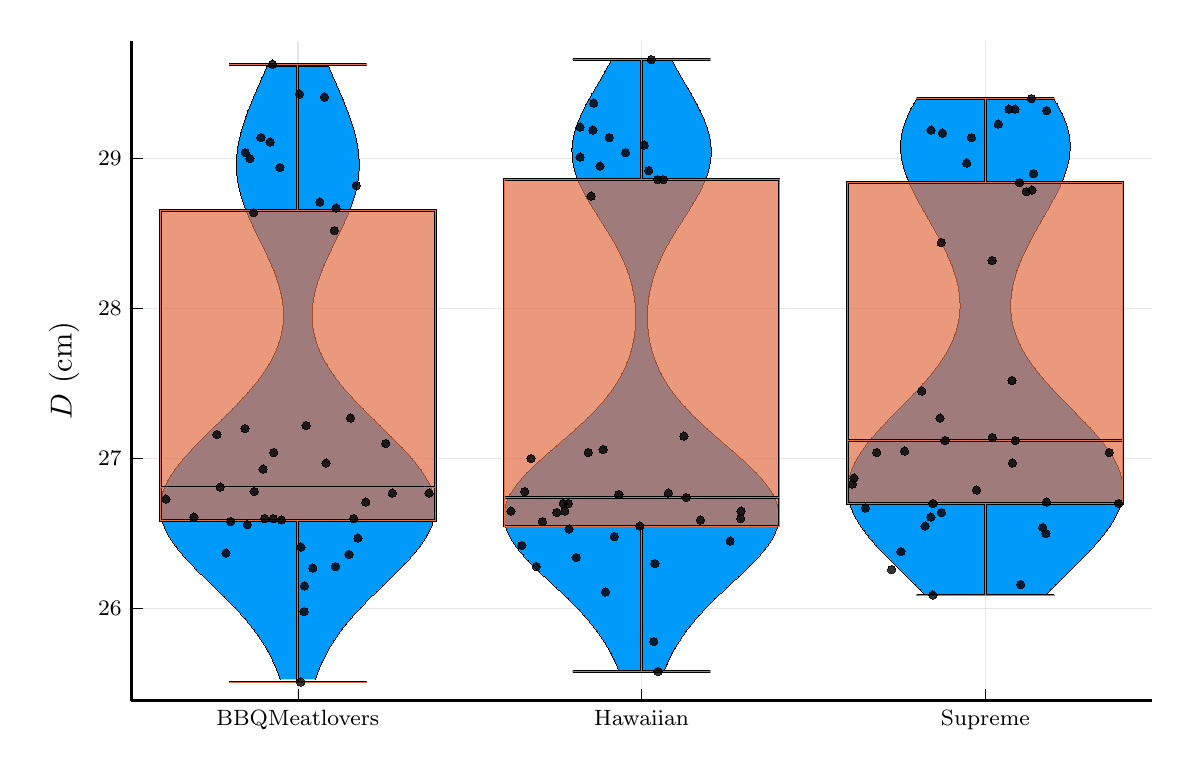
\begin{tikzpicture}[/tikz/background rectangle/.style={fill={rgb,1:red,1.0;green,1.0;blue,1.0}, draw opacity={1.0}}, show background rectangle]
\begin{axis}[point meta max={nan}, point meta min={nan}, title={}, title style={at={{(0.5,1)}}, anchor={south}, font={{\fontsize{14 pt}{18.2 pt}\selectfont}}, color={rgb,1:red,0.0;green,0.0;blue,0.0}, draw opacity={1.0}, rotate={0.0}}, legend style={color={rgb,1:red,0.0;green,0.0;blue,0.0}, draw opacity={1.0}, line width={1}, solid, fill={rgb,1:red,1.0;green,1.0;blue,1.0}, fill opacity={1.0}, text opacity={1.0}, font={{\fontsize{8 pt}{10.4 pt}\selectfont}}, text={rgb,1:red,0.0;green,0.0;blue,0.0}, cells={anchor={center}}, at={(1.02, 1)}, anchor={north west}}, axis background/.style={fill={rgb,1:red,1.0;green,1.0;blue,1.0}, opacity={1.0}}, anchor={north west}, xshift={1.0mm}, yshift={-1.0mm}, width={145.4mm}, height={99.6mm}, scaled x ticks={false}, xlabel={}, x tick style={color={rgb,1:red,0.0;green,0.0;blue,0.0}, opacity={1.0}}, x tick label style={color={rgb,1:red,0.0;green,0.0;blue,0.0}, opacity={1.0}, rotate={0}}, xlabel style={at={(ticklabel cs:0.5)}, anchor=near ticklabel, at={{(ticklabel cs:0.5)}}, anchor={near ticklabel}, font={{\fontsize{11 pt}{14.3 pt}\selectfont}}, color={rgb,1:red,0.0;green,0.0;blue,0.0}, draw opacity={1.0}, rotate={0.0}}, xmajorgrids={true}, xmin={0.015999999999999986}, xmax={2.984}, xtick={{0.5,1.5,2.5}}, xticklabels={{BBQMeatlovers,Hawaiian,Supreme}}, xtick align={inside}, xticklabel style={font={{\fontsize{8 pt}{10.4 pt}\selectfont}}, color={rgb,1:red,0.0;green,0.0;blue,0.0}, draw opacity={1.0}, rotate={0.0}}, x grid style={color={rgb,1:red,0.0;green,0.0;blue,0.0}, draw opacity={0.1}, line width={0.5}, solid}, axis x line*={left}, x axis line style={color={rgb,1:red,0.0;green,0.0;blue,0.0}, draw opacity={1.0}, line width={1}, solid}, scaled y ticks={false}, ylabel={$D$ (cm)}, y tick style={color={rgb,1:red,0.0;green,0.0;blue,0.0}, opacity={1.0}}, y tick label style={color={rgb,1:red,0.0;green,0.0;blue,0.0}, opacity={1.0}, rotate={0}}, ylabel style={at={(ticklabel cs:0.5)}, anchor=near ticklabel, at={{(ticklabel cs:0.5)}}, anchor={near ticklabel}, font={{\fontsize{11 pt}{14.3 pt}\selectfont}}, color={rgb,1:red,0.0;green,0.0;blue,0.0}, draw opacity={1.0}, rotate={0.0}}, ymajorgrids={true}, ymin={25.3855}, ymax={29.7845}, ytick={{26.0,27.0,28.0,29.0}}, yticklabels={{$26$,$27$,$28$,$29$}}, ytick align={inside}, yticklabel style={font={{\fontsize{8 pt}{10.4 pt}\selectfont}}, color={rgb,1:red,0.0;green,0.0;blue,0.0}, draw opacity={1.0}, rotate={0.0}}, y grid style={color={rgb,1:red,0.0;green,0.0;blue,0.0}, draw opacity={0.1}, line width={0.5}, solid}, axis y line*={left}, y axis line style={color={rgb,1:red,0.0;green,0.0;blue,0.0}, draw opacity={1.0}, line width={1}, solid}, colorbar={false}]
    \addplot[color={rgb,1:red,0.0;green,0.0;blue,0.0}, name path={b758c778-50e9-4ec9-af20-0296ee405787}, area legend, fill={rgb,1:red,0.0;green,0.6056;blue,0.9787}, fill opacity={1.0}, draw opacity={1.0}, line width={0}, solid, forget plot]
        table[row sep={\\}]
        {
            \\
            0.5508782171085028  25.527172604634924  \\
            0.5564972557085687  25.56398030545231  \\
            0.5627197966641814  25.600788006269703  \\
            0.5696018222099328  25.63759570708709  \\
            0.5771970479819148  25.674403407904478  \\
            0.5855546914189029  25.71121110872187  \\
            0.5947170573062931  25.748018809539257  \\
            0.6047170190645681  25.784826510356645  \\
            0.615575486950734  25.821634211174032  \\
            0.6272989637802462  25.858441911991424  \\
            0.6398772944763109  25.89524961280881  \\
            0.6532817172156722  25.9320573136262  \\
            0.667463320796025  25.96886501444359  \\
            0.6823520048755654  26.005672715260978  \\
            0.6978560268705727  26.042480416078366  \\
            0.7138622016743597  26.079288116895754  \\
            0.7302367983333795  26.116095817713145  \\
            0.7468271519867171  26.152903518530533  \\
            0.7634639806180806  26.18971121934792  \\
            0.7799643656373143  26.22651892016531  \\
            0.7961353244150329  26.2633266209827  \\
            0.8117778732675243  26.300134321800087  \\
            0.8266914527925745  26.336942022617478  \\
            0.8406785656758788  26.373749723434866  \\
            0.8535494617917254  26.410557424252254  \\
            0.8651266980103575  26.44736512506964  \\
            0.875249401574402  26.484172825887033  \\
            0.8837770766366979  26.52098052670442  \\
            0.8905928133256469  26.557788227521808  \\
            0.8956057865880622  26.5945959283392  \\
            0.8987529664454508  26.631403629156587  \\
            0.9  26.668211329973975  \\
            0.8993412659355464  26.705019030791366  \\
            0.8967991415692086  26.741826731608754  \\
            0.8924225579629629  26.77863443242614  \\
            0.8862849477502337  26.81544213324353  \\
            0.8784817112634519  26.85224983406092  \\
            0.869127338087987  26.889057534878308  \\
            0.8583523229834649  26.925865235695696  \\
            0.8463000077417502  26.962672936513087  \\
            0.8331234653287407  26.999480637330475  \\
            0.8189825215666922  27.036288338147862  \\
            0.8040409850581538  27.07309603896525  \\
            0.7884641305889384  27.10990373978264  \\
            0.7724164573095791  27.14671144060003  \\
            0.7560597226375771  27.183519141417417  \\
            0.7395512375201909  27.220326842234808  \\
            0.7230423992148973  27.257134543052196  \\
            0.7066774341001968  27.293942243869584  \\
            0.690592324545945  27.330749944686975  \\
            0.6749138993094048  27.367557645504363  \\
            0.6597590746698738  27.40436534632175  \\
            0.6452342418174297  27.441173047139138  \\
            0.6314348032057819  27.47798074795653  \\
            0.6184448652988062  27.514788448773917  \\
            0.6063370964758685  27.551596149591305  \\
            0.5951727564549479  27.588403850408696  \\
            0.5850018976596997  27.625211551226084  \\
            0.5758637302329663  27.66201925204347  \\
            0.5677871320289063  27.698826952860863  \\
            0.5607912742932549  27.73563465367825  \\
            0.5548863243295257  27.772442354495638  \\
            0.5500741795981894  27.809250055313026  \\
            0.5463491844808038  27.846057756130417  \\
            0.543698782036949  27.882865456947805  \\
            0.5421040586897846  27.919673157765192  \\
            0.5415401496035963  27.956480858582584  \\
            0.5419764858126743  27.99328855939997  \\
            0.5433768797981707  28.03009626021736  \\
            0.5456994628045905  28.06690396103475  \\
            0.5488965032420853  28.103711661852138  \\
            0.552914149570916  28.140519362669526  \\
            0.5576921518216508  28.177327063486914  \\
            0.5631636223744192  28.214134764304305  \\
            0.5692548981895418  28.250942465121692  \\
            0.5758855631657649  28.28775016593908  \\
            0.5829686809519802  28.32455786675647  \\
            0.5904112760055269  28.36136556757386  \\
            0.5981150849587135  28.398173268391247  \\
            0.6059775826449716  28.434980969208635  \\
            0.6138932687911722  28.471788670026026  \\
            0.6217551837547147  28.508596370843414  \\
            0.629456606021883  28.5454040716608  \\
            0.636892871539637  28.582211772478193  \\
            0.6439632461111421  28.61901947329558  \\
            0.6505727775208641  28.655827174112968  \\
            0.6566340539198225  28.69263487493036  \\
            0.6620687991383009  28.729442575747747  \\
            0.6668092435719568  28.766250276565135  \\
            0.6707992204581179  28.803057977382522  \\
            0.6739949509148087  28.839865678199914  \\
            0.6763654961561544  28.8766733790173  \\
            0.677892870894489  28.91348107983469  \\
            0.6785718271875951  28.95028878065208  \\
            0.6784093320572296  28.987096481469468  \\
            0.6774237743707523  29.023904182286856  \\
            0.6756439461587987  29.060711883104247  \\
            0.6731078503170669  29.097519583921635  \\
            0.6698613902643052  29.134327284739022  \\
            0.6659569975420729  29.17113498555641  \\
            0.6614522506735953  29.2079426863738  \\
            0.6564085331607624  29.24475038719119  \\
            0.6508897707693098  29.281558088008577  \\
            0.6449612788529069  29.318365788825968  \\
            0.6386887401203593  29.355173489643356  \\
            0.6321373227326306  29.391981190460744  \\
            0.6253709386995706  29.42878889127813  \\
            0.6184516339354313  29.465596592095523  \\
            0.6114390946070907  29.50240429291291  \\
            0.6043902499723419  29.539211993730298  \\
            0.5973589499481031  29.57601969454769  \\
            0.5903956961318377  29.612827395365077  \\
            0.40960430386816227  29.612827395365077  \\
            0.4026410500518969  29.57601969454769  \\
            0.395609750027658  29.539211993730298  \\
            0.38856090539290933  29.50240429291291  \\
            0.38154836606456866  29.465596592095523  \\
            0.3746290613004294  29.42878889127813  \\
            0.36786267726736943  29.391981190460744  \\
            0.36131125987964074  29.355173489643356  \\
            0.3550387211470931  29.318365788825968  \\
            0.34911022923069024  29.281558088008577  \\
            0.3435914668392376  29.24475038719119  \\
            0.33854774932640475  29.2079426863738  \\
            0.33404300245792706  29.17113498555641  \\
            0.33013860973569475  29.134327284739022  \\
            0.3268921496829331  29.097519583921635  \\
            0.32435605384120125  29.060711883104247  \\
            0.3225762256292477  29.023904182286856  \\
            0.32159066794277036  28.987096481469468  \\
            0.3214281728124049  28.95028878065208  \\
            0.322107129105511  28.91348107983469  \\
            0.3236345038438456  28.8766733790173  \\
            0.32600504908519135  28.839865678199914  \\
            0.3292007795418821  28.803057977382522  \\
            0.33319075642804324  28.766250276565135  \\
            0.33793120086169914  28.729442575747747  \\
            0.3433659460801774  28.69263487493036  \\
            0.34942722247913593  28.655827174112968  \\
            0.3560367538888579  28.61901947329558  \\
            0.36310712846036297  28.582211772478193  \\
            0.370543393978117  28.5454040716608  \\
            0.3782448162452853  28.508596370843414  \\
            0.3861067312088277  28.471788670026026  \\
            0.39402241735502835  28.434980969208635  \\
            0.4018849150412866  28.398173268391247  \\
            0.40958872399447316  28.36136556757386  \\
            0.4170313190480198  28.32455786675647  \\
            0.4241144368342351  28.28775016593908  \\
            0.43074510181045816  28.250942465121692  \\
            0.43683637762558086  28.214134764304305  \\
            0.4423078481783493  28.177327063486914  \\
            0.447085850429084  28.140519362669526  \\
            0.4511034967579147  28.103711661852138  \\
            0.4543005371954095  28.06690396103475  \\
            0.45662312020182927  28.03009626021736  \\
            0.4580235141873256  27.99328855939997  \\
            0.45845985039640363  27.956480858582584  \\
            0.4578959413102154  27.919673157765192  \\
            0.456301217963051  27.882865456947805  \\
            0.45365081551919617  27.846057756130417  \\
            0.4499258204018106  27.809250055313026  \\
            0.44511367567047433  27.772442354495638  \\
            0.43920872570674513  27.73563465367825  \\
            0.43221286797109376  27.698826952860863  \\
            0.42413626976703367  27.66201925204347  \\
            0.4149981023403003  27.625211551226084  \\
            0.4048272435450521  27.588403850408696  \\
            0.3936629035241314  27.551596149591305  \\
            0.3815551347011939  27.514788448773917  \\
            0.36856519679421806  27.47798074795653  \\
            0.3547657581825702  27.441173047139138  \\
            0.3402409253301262  27.40436534632175  \\
            0.3250861006905952  27.367557645504363  \\
            0.309407675454055  27.330749944686975  \\
            0.2933225658998032  27.293942243869584  \\
            0.2769576007851026  27.257134543052196  \\
            0.26044876247980914  27.220326842234808  \\
            0.2439402773624228  27.183519141417417  \\
            0.22758354269042097  27.14671144060003  \\
            0.21153586941106167  27.10990373978264  \\
            0.1959590149418462  27.07309603896525  \\
            0.1810174784333079  27.036288338147862  \\
            0.1668765346712593  26.999480637330475  \\
            0.15369999225824987  26.962672936513087  \\
            0.14164767701653508  26.925865235695696  \\
            0.13087266191201297  26.889057534878308  \\
            0.12151828873654813  26.85224983406092  \\
            0.1137150522497663  26.81544213324353  \\
            0.10757744203703712  26.77863443242614  \\
            0.10320085843079141  26.741826731608754  \\
            0.10065873406445364  26.705019030791366  \\
            0.09999999999999998  26.668211329973975  \\
            0.10124703355454917  26.631403629156587  \\
            0.10439421341193772  26.5945959283392  \\
            0.10940718667435312  26.557788227521808  \\
            0.11622292336330203  26.52098052670442  \\
            0.12475059842559799  26.484172825887033  \\
            0.13487330198964254  26.44736512506964  \\
            0.14645053820827464  26.410557424252254  \\
            0.1593214343241211  26.373749723434866  \\
            0.1733085472074255  26.336942022617478  \\
            0.18822212673247574  26.300134321800087  \\
            0.20386467558496718  26.2633266209827  \\
            0.22003563436268575  26.22651892016531  \\
            0.23653601938191937  26.18971121934792  \\
            0.2531728480132829  26.152903518530533  \\
            0.26976320166662043  26.116095817713145  \\
            0.28613779832564035  26.079288116895754  \\
            0.3021439731294273  26.042480416078366  \\
            0.31764799512443465  26.005672715260978  \\
            0.33253667920397495  25.96886501444359  \\
            0.3467182827843278  25.9320573136262  \\
            0.3601227055236891  25.89524961280881  \\
            0.3727010362197538  25.858441911991424  \\
            0.38442451304926595  25.821634211174032  \\
            0.3952829809354319  25.784826510356645  \\
            0.4052829426937069  25.748018809539257  \\
            0.4144453085810971  25.71121110872187  \\
            0.4228029520180851  25.674403407904478  \\
            0.4303981777900671  25.63759570708709  \\
            0.43728020333581863  25.600788006269703  \\
            0.44350274429143133  25.56398030545231  \\
            0.44912178289149723  25.527172604634924  \\
        }
        ;
    \addplot[color={rgb,1:red,0.0;green,0.0;blue,0.0}, name path={b758c778-50e9-4ec9-af20-0296ee405787}, area legend, fill={rgb,1:red,0.0;green,0.6056;blue,0.9787}, fill opacity={1.0}, draw opacity={1.0}, line width={0}, solid, forget plot]
        table[row sep={\\}]
        {
            \\
            1.566201692981847  25.588328383529394  \\
            1.5728924621404097  25.624935079321656  \\
            1.5802002522941716  25.66154177511392  \\
            1.5881836039930373  25.698148470906183  \\
            1.5968998734901034  25.734755166698445  \\
            1.6064023993374827  25.77136186249071  \\
            1.6167372764612233  25.807968558282973  \\
            1.627939843346825  25.844575254075234  \\
            1.6400310191536882  25.8811819498675  \\
            1.6530136545247702  25.917788645659762  \\
            1.6668690803930704  25.954395341452024  \\
            1.6815540512126548  25.99100203724429  \\
            1.6969982810912845  26.02760873303655  \\
            1.7131027620837649  26.064215428828813  \\
            1.729739032839295  26.10082212462108  \\
            1.7467495330182459  26.13742882041334  \\
            1.7639491353250953  26.174035516205606  \\
            1.7811278943706736  26.210642211997868  \\
            1.7980549923711981  26.24724890779013  \\
            1.814483799071595  26.283855603582396  \\
            1.830157900903626  26.320462299374658  \\
            1.8448178961878923  26.35706899516692  \\
            1.8582087030999723  26.393675690959185  \\
            1.8700870887880428  26.430282386751447  \\
            1.8802291044999675  26.46688908254371  \\
            1.8884371050268267  26.503495778335974  \\
            1.8945460422751257  26.540102474128236  \\
            1.89842875217824  26.5767091699205  \\
            1.9  26.613315865712764  \\
            1.8992191087017072  26.649922561505026  \\
            1.8960910647293037  26.686529257297288  \\
            1.8906660708571763  26.723135953089553  \\
            1.8830375917157667  26.759742648881815  \\
            1.8733390094334412  26.796349344674077  \\
            1.8617390699253493  26.832956040466343  \\
            1.8484363509981452  26.869562736258604  \\
            1.833653018883544  26.906169432050866  \\
            1.817628158568473  26.942776127843132  \\
            1.800610965157086  26.979382823635394  \\
            1.7828540695297002  27.015989519427656  \\
            1.7646072438885099  27.05259621521992  \\
            1.746111694361176  27.089202911012183  \\
            1.727595102147304  27.125809606804445  \\
            1.7092675253939373  27.16241630259671  \\
            1.6913182245837264  27.199022998388973  \\
            1.6739134277994299  27.235629694181235  \\
            1.6571950112455103  27.2722363899735  \\
            1.6412800365605313  27.308843085765762  \\
            1.6262610606486858  27.345449781558024  \\
            1.612207116150697  27.38205647735029  \\
            1.5991652507770309  27.41866317314255  \\
            1.5871625105632576  27.455269868934813  \\
            1.5762082543860938  27.49187656472708  \\
            1.5662966933648141  27.52848326051934  \\
            1.55740955764646  27.565089956311603  \\
            1.5495188032545042  27.60169665210387  \\
            1.5425892821169112  27.63830334789613  \\
            1.5365813083052369  27.674910043688396  \\
            1.5314530624264706  27.711516739480658  \\
            1.5271627838047686  27.74812343527292  \\
            1.5236707066029918  27.784730131065185  \\
            1.5209407015897916  27.821336826857447  \\
            1.518941590223696  27.85794352264971  \\
            1.517648102555953  27.894550218441974  \\
            1.5170414556404956  27.931156914234236  \\
            1.5171095351632922  27.9677636100265  \\
            1.5178466702901439  28.004370305818764  \\
            1.5192530006100795  28.040977001611026  \\
            1.5213334447124123  28.077583697403288  \\
            1.524096292398458  28.114190393195553  \\
            1.5275514566107242  28.150797088987815  \\
            1.5317084364573537  28.187403784780077  \\
            1.5365740585830887  28.224010480572343  \\
            1.542150079737968  28.260617176364605  \\
            1.5484307476854766  28.297223872156867  \\
            1.5554004294099255  28.333830567949132  \\
            1.5630314237178593  28.370437263741394  \\
            1.5712820786207218  28.407043959533656  \\
            1.5800953313381563  28.44365065532592  \\
            1.589397779651188  28.480257351118183  \\
            1.5990993773213014  28.516864046910445  \\
            1.6090938235003969  28.55347074270271  \\
            1.6192596871324827  28.590077438494973  \\
            1.6294622734666078  28.626684134287235  \\
            1.6395562026336952  28.6632908300795  \\
            1.649388631870733  28.699897525871762  \\
            1.658803015768953  28.736504221664024  \\
            1.6676432653575561  28.77311091745629  \\
            1.6757581393142393  28.80971761324855  \\
            1.6830056812464034  28.846324309040813  \\
            1.689257507477813  28.88293100483308  \\
            1.694402751148577  28.91953770062534  \\
            1.6983514810007927  28.956144396417603  \\
            1.7010374364975989  28.99275109220987  \\
            1.7024199536502436  29.02935778800213  \\
            1.7024849961452255  29.065964483794392  \\
            1.701245251548708  29.102571179586658  \\
            1.6987392996227606  29.13917787537892  \\
            1.6950299060729488  29.175784571171185  \\
            1.6902015374028687  29.212391266963447  \\
            1.6843572283395667  29.24899796275571  \\
            1.6776149603944792  29.285604658547975  \\
            1.6701037270915033  29.322211354340237  \\
            1.661959467549879  29.3588180501325  \\
            1.6533210455744454  29.395424745924764  \\
            1.6443264370559163  29.432031441717026  \\
            1.6351092658495137  29.468638137509288  \\
            1.6257957994126095  29.505244833301553  \\
            1.6165024826840895  29.541851529093815  \\
            1.607334054430811  29.578458224886077  \\
            1.5983822569273505  29.615064920678343  \\
            1.589725119459028  29.651671616470605  \\
            1.410274880540972  29.651671616470605  \\
            1.4016177430726495  29.615064920678343  \\
            1.392665945569189  29.578458224886077  \\
            1.3834975173159105  29.541851529093815  \\
            1.3742042005873905  29.505244833301553  \\
            1.3648907341504863  29.468638137509288  \\
            1.3556735629440837  29.432031441717026  \\
            1.3466789544255546  29.395424745924764  \\
            1.338040532450121  29.3588180501325  \\
            1.3298962729084967  29.322211354340237  \\
            1.3223850396055208  29.285604658547975  \\
            1.3156427716604333  29.24899796275571  \\
            1.3097984625971313  29.212391266963447  \\
            1.3049700939270512  29.175784571171185  \\
            1.3012607003772394  29.13917787537892  \\
            1.298754748451292  29.102571179586658  \\
            1.2975150038547745  29.065964483794392  \\
            1.2975800463497564  29.02935778800213  \\
            1.2989625635024011  28.99275109220987  \\
            1.3016485189992073  28.956144396417603  \\
            1.305597248851423  28.91953770062534  \\
            1.310742492522187  28.88293100483308  \\
            1.3169943187535966  28.846324309040813  \\
            1.3242418606857607  28.80971761324855  \\
            1.3323567346424439  28.77311091745629  \\
            1.341196984231047  28.736504221664024  \\
            1.350611368129267  28.699897525871762  \\
            1.3604437973663048  28.6632908300795  \\
            1.3705377265333922  28.626684134287235  \\
            1.3807403128675173  28.590077438494973  \\
            1.3909061764996031  28.55347074270271  \\
            1.4009006226786986  28.516864046910445  \\
            1.410602220348812  28.480257351118183  \\
            1.4199046686618437  28.44365065532592  \\
            1.4287179213792782  28.407043959533656  \\
            1.4369685762821407  28.370437263741394  \\
            1.4445995705900745  28.333830567949132  \\
            1.4515692523145234  28.297223872156867  \\
            1.457849920262032  28.260617176364605  \\
            1.4634259414169113  28.224010480572343  \\
            1.4682915635426463  28.187403784780077  \\
            1.4724485433892758  28.150797088987815  \\
            1.475903707601542  28.114190393195553  \\
            1.4786665552875877  28.077583697403288  \\
            1.4807469993899205  28.040977001611026  \\
            1.4821533297098561  28.004370305818764  \\
            1.4828904648367078  27.9677636100265  \\
            1.4829585443595044  27.931156914234236  \\
            1.482351897444047  27.894550218441974  \\
            1.481058409776304  27.85794352264971  \\
            1.4790592984102084  27.821336826857447  \\
            1.4763292933970082  27.784730131065185  \\
            1.4728372161952314  27.74812343527292  \\
            1.4685469375735294  27.711516739480658  \\
            1.4634186916947631  27.674910043688396  \\
            1.4574107178830888  27.63830334789613  \\
            1.4504811967454958  27.60169665210387  \\
            1.44259044235354  27.565089956311603  \\
            1.4337033066351859  27.52848326051934  \\
            1.4237917456139062  27.49187656472708  \\
            1.4128374894367424  27.455269868934813  \\
            1.4008347492229691  27.41866317314255  \\
            1.387792883849303  27.38205647735029  \\
            1.3737389393513142  27.345449781558024  \\
            1.3587199634394687  27.308843085765762  \\
            1.3428049887544897  27.2722363899735  \\
            1.3260865722005701  27.235629694181235  \\
            1.3086817754162736  27.199022998388973  \\
            1.2907324746060627  27.16241630259671  \\
            1.272404897852696  27.125809606804445  \\
            1.253888305638824  27.089202911012183  \\
            1.2353927561114901  27.05259621521992  \\
            1.2171459304702998  27.015989519427656  \\
            1.199389034842914  26.979382823635394  \\
            1.182371841431527  26.942776127843132  \\
            1.166346981116456  26.906169432050866  \\
            1.1515636490018548  26.869562736258604  \\
            1.1382609300746507  26.832956040466343  \\
            1.1266609905665588  26.796349344674077  \\
            1.1169624082842333  26.759742648881815  \\
            1.1093339291428237  26.723135953089553  \\
            1.1039089352706963  26.686529257297288  \\
            1.1007808912982928  26.649922561505026  \\
            1.1  26.613315865712764  \\
            1.10157124782176  26.5767091699205  \\
            1.1054539577248743  26.540102474128236  \\
            1.1115628949731733  26.503495778335974  \\
            1.1197708955000325  26.46688908254371  \\
            1.1299129112119572  26.430282386751447  \\
            1.1417912969000277  26.393675690959185  \\
            1.1551821038121077  26.35706899516692  \\
            1.169842099096374  26.320462299374658  \\
            1.185516200928405  26.283855603582396  \\
            1.2019450076288019  26.24724890779013  \\
            1.2188721056293264  26.210642211997868  \\
            1.2360508646749047  26.174035516205606  \\
            1.2532504669817541  26.13742882041334  \\
            1.270260967160705  26.10082212462108  \\
            1.2868972379162351  26.064215428828813  \\
            1.3030017189087155  26.02760873303655  \\
            1.3184459487873452  25.99100203724429  \\
            1.3331309196069296  25.954395341452024  \\
            1.3469863454752298  25.917788645659762  \\
            1.3599689808463118  25.8811819498675  \\
            1.372060156653175  25.844575254075234  \\
            1.3832627235387767  25.807968558282973  \\
            1.3935976006625173  25.77136186249071  \\
            1.4031001265098966  25.734755166698445  \\
            1.4118163960069627  25.698148470906183  \\
            1.4197997477058284  25.66154177511392  \\
            1.4271075378595903  25.624935079321656  \\
            1.433798307018153  25.588328383529394  \\
        }
        ;
    \addplot[color={rgb,1:red,0.0;green,0.0;blue,0.0}, name path={b758c778-50e9-4ec9-af20-0296ee405787}, area legend, fill={rgb,1:red,0.0;green,0.6056;blue,0.9787}, fill opacity={1.0}, draw opacity={1.0}, line width={0}, solid, forget plot]
        table[row sep={\\}]
        {
            \\
            2.676237714187736  26.091763872540962  \\
            2.6899871236787076  26.124501221599555  \\
            2.704048421209403  26.15723857065815  \\
            2.718343336155128  26.189975919716748  \\
            2.732785659216785  26.22271326877534  \\
            2.7472818411165036  26.255450617833937  \\
            2.761731778230355  26.28818796689253  \\
            2.7760297867319808  26.320925315951126  \\
            2.7900657602818715  26.353662665009722  \\
            2.803726499104493  26.386400014068315  \\
            2.816897190846222  26.41913736312691  \\
            2.8294630163521726  26.451874712185504  \\
            2.841310846908537  26.4846120612441  \\
            2.852330994016096  26.517349410302693  \\
            2.862418968776484  26.55008675936129  \\
            2.8714772057769884  26.582824108419885  \\
            2.8794167061230436  26.615561457478478  \\
            2.88615855602626  26.648298806537074  \\
            2.89163528100927  26.681036155595667  \\
            2.8957920011105887  26.713773504654263  \\
            2.8985873591334252  26.74651085371286  \\
            2.899994201579211  26.779248202771452  \\
            2.9  26.81198555183005  \\
            2.898607008654097  26.84472290088864  \\
            2.8958321621505667  26.877460249947237  \\
            2.8917067238770287  26.910197599005834  \\
            2.8862757021591756  26.942934948064426  \\
            2.8795970561287167  26.975672297123023  \\
            2.8717407170990117  27.008409646181615  \\
            2.8627874538668965  27.04114699524021  \\
            2.852827611844689  27.073884344298804  \\
            2.841959756395926  27.1066216933574  \\
            2.8302892503480654  27.139359042415997  \\
            2.8179267945412954  27.17209639147459  \\
            2.8049869585959835  27.204833740533186  \\
            2.791586726978942  27.23757108959178  \\
            2.7778440830380515  27.270308438650375  \\
            2.7638766510538697  27.30304578770897  \\
            2.7498004136076037  27.335783136767564  \\
            2.7357285187581475  27.36852048582616  \\
            2.721770188721782  27.401257834884753  \\
            2.7080297390195835  27.43399518394335  \\
            2.69460571446183  27.466732533001945  \\
            2.6815901459357248  27.499469882060538  \\
            2.669067929806201  27.532207231119134  \\
            2.657116329870684  27.564944580177727  \\
            2.645804600249767  27.597681929236323  \\
            2.6351937263445664  27.630419278294916  \\
            2.625336280017666  27.663156627353512  \\
            2.616276384399688  27.69589397641211  \\
            2.6080497831051495  27.7286313254707  \\
            2.6006840080606946  27.761368674529297  \\
            2.594198639502751  27.79410602358789  \\
            2.5886056508955346  27.826843372646486  \\
            2.5839098304826673  27.859580721705083  \\
            2.5801092698808237  27.892318070763675  \\
            2.5771959085620697  27.92505541982227  \\
            2.5751561213142398  27.957792768880864  \\
            2.5739713339281383  27.99053011793946  \\
            2.573618650593336  28.023267466998053  \\
            2.5740714749803004  28.05600481605665  \\
            2.5753001059507374  28.088742165115246  \\
            2.577272288471393  28.12147951417384  \\
            2.579953700785102  28.154216863232435  \\
            2.583308360347308  28.186954212291027  \\
            2.587298933535325  28.219691561349624  \\
            2.5918869376764446  28.25242891040822  \\
            2.5970328284354256  28.285166259466813  \\
            2.602695970890528  28.31790360852541  \\
            2.6088344984794976  28.350640957584  \\
            2.615405070127871  28.383378306642598  \\
            2.622362541961371  28.416115655701194  \\
            2.629659575718075  28.448853004759787  \\
            2.637246210989232  28.481590353818383  \\
            2.6450694324340502  28.514327702876976  \\
            2.6530727658840974  28.547065051935572  \\
            2.661195938587316  28.579802400994165  \\
            2.669374638617277  28.61253975005276  \\
            2.677540406637378  28.645277099111357  \\
            2.6856206897777275  28.67801444816995  \\
            2.693539082433636  28.710751797228546  \\
            2.7012157724653894  28.74348914628714  \\
            2.7085682037565117  28.776226495345735  \\
            2.7155119576037556  28.80896384440433  \\
            2.72196184623838  28.841701193462924  \\
            2.7278332022231684  28.87443854252152  \\
            2.7330433378748227  28.907175891580113  \\
            2.737513139598704  28.93991324063871  \\
            2.741168753488136  28.972650589697306  \\
            2.743943311144469  29.0053879387559  \\
            2.7457786388281544  29.038125287814495  \\
            2.7466268891480583  29.070862636873088  \\
            2.7464520328860873  29.103599985931684  \\
            2.745231149516379  29.136337334990277  \\
            2.742955458692761  29.169074684048873  \\
            2.739631041498009  29.20181203310747  \\
            2.735279209477851  29.234549382166062  \\
            2.729936491163131  29.267286731224658  \\
            2.723654219491592  29.30002408028325  \\
            2.7164977186986485  29.332761429341847  \\
            2.7085451051474743  29.365498778400443  \\
            2.6998857324144754  29.398236127459036  \\
            2.3001142675855246  29.398236127459036  \\
            2.2914548948525257  29.365498778400443  \\
            2.2835022813013515  29.332761429341847  \\
            2.276345780508408  29.30002408028325  \\
            2.270063508836869  29.267286731224658  \\
            2.264720790522149  29.234549382166062  \\
            2.260368958501991  29.20181203310747  \\
            2.257044541307239  29.169074684048873  \\
            2.254768850483621  29.136337334990277  \\
            2.2535479671139127  29.103599985931684  \\
            2.2533731108519417  29.070862636873088  \\
            2.2542213611718456  29.038125287814495  \\
            2.256056688855531  29.0053879387559  \\
            2.258831246511864  28.972650589697306  \\
            2.262486860401296  28.93991324063871  \\
            2.2669566621251773  28.907175891580113  \\
            2.2721667977768316  28.87443854252152  \\
            2.27803815376162  28.841701193462924  \\
            2.2844880423962444  28.80896384440433  \\
            2.2914317962434883  28.776226495345735  \\
            2.2987842275346106  28.74348914628714  \\
            2.306460917566364  28.710751797228546  \\
            2.3143793102222725  28.67801444816995  \\
            2.322459593362622  28.645277099111357  \\
            2.330625361382723  28.61253975005276  \\
            2.338804061412684  28.579802400994165  \\
            2.3469272341159026  28.547065051935572  \\
            2.3549305675659498  28.514327702876976  \\
            2.362753789010768  28.481590353818383  \\
            2.370340424281925  28.448853004759787  \\
            2.377637458038629  28.416115655701194  \\
            2.384594929872129  28.383378306642598  \\
            2.3911655015205024  28.350640957584  \\
            2.397304029109472  28.31790360852541  \\
            2.4029671715645744  28.285166259466813  \\
            2.4081130623235554  28.25242891040822  \\
            2.412701066464675  28.219691561349624  \\
            2.416691639652692  28.186954212291027  \\
            2.420046299214898  28.154216863232435  \\
            2.422727711528607  28.12147951417384  \\
            2.4246998940492626  28.088742165115246  \\
            2.4259285250196996  28.05600481605665  \\
            2.426381349406664  28.023267466998053  \\
            2.4260286660718617  27.99053011793946  \\
            2.4248438786857602  27.957792768880864  \\
            2.4228040914379303  27.92505541982227  \\
            2.4198907301191763  27.892318070763675  \\
            2.4160901695173327  27.859580721705083  \\
            2.4113943491044654  27.826843372646486  \\
            2.405801360497249  27.79410602358789  \\
            2.3993159919393054  27.761368674529297  \\
            2.3919502168948505  27.7286313254707  \\
            2.383723615600312  27.69589397641211  \\
            2.374663719982334  27.663156627353512  \\
            2.3648062736554336  27.630419278294916  \\
            2.354195399750233  27.597681929236323  \\
            2.342883670129316  27.564944580177727  \\
            2.330932070193799  27.532207231119134  \\
            2.3184098540642752  27.499469882060538  \\
            2.30539428553817  27.466732533001945  \\
            2.2919702609804165  27.43399518394335  \\
            2.278229811278218  27.401257834884753  \\
            2.2642714812418525  27.36852048582616  \\
            2.2501995863923963  27.335783136767564  \\
            2.2361233489461303  27.30304578770897  \\
            2.2221559169619485  27.270308438650375  \\
            2.208413273021058  27.23757108959178  \\
            2.1950130414040165  27.204833740533186  \\
            2.1820732054587046  27.17209639147459  \\
            2.1697107496519346  27.139359042415997  \\
            2.158040243604074  27.1066216933574  \\
            2.147172388155311  27.073884344298804  \\
            2.1372125461331035  27.04114699524021  \\
            2.1282592829009883  27.008409646181615  \\
            2.1204029438712833  26.975672297123023  \\
            2.1137242978408244  26.942934948064426  \\
            2.1082932761229713  26.910197599005834  \\
            2.1041678378494333  26.877460249947237  \\
            2.101392991345903  26.84472290088864  \\
            2.1  26.81198555183005  \\
            2.100005798420789  26.779248202771452  \\
            2.1014126408665748  26.74651085371286  \\
            2.1042079988894113  26.713773504654263  \\
            2.10836471899073  26.681036155595667  \\
            2.11384144397374  26.648298806537074  \\
            2.1205832938769564  26.615561457478478  \\
            2.1285227942230116  26.582824108419885  \\
            2.137581031223516  26.55008675936129  \\
            2.147669005983904  26.517349410302693  \\
            2.158689153091463  26.4846120612441  \\
            2.1705369836478274  26.451874712185504  \\
            2.183102809153778  26.41913736312691  \\
            2.196273500895507  26.386400014068315  \\
            2.2099342397181285  26.353662665009722  \\
            2.2239702132680192  26.320925315951126  \\
            2.238268221769645  26.28818796689253  \\
            2.2527181588834964  26.255450617833937  \\
            2.267214340783215  26.22271326877534  \\
            2.281656663844872  26.189975919716748  \\
            2.295951578790597  26.15723857065815  \\
            2.3100128763212924  26.124501221599555  \\
            2.323762285812264  26.091763872540962  \\
        }
        ;
    \addplot[color={rgb,1:red,0.0;green,0.0;blue,0.0}, name path={e1805b5c-e9da-4ac7-9b44-3491654c5491}, area legend, fill={rgb,1:red,0.8889;green,0.4356;blue,0.2781}, fill opacity={0.7}, draw opacity={1.0}, line width={1}, solid, forget plot]
        table[row sep={\\}]
        {
            \\
            0.5  25.51  \\
            0.3  25.51  \\
            0.7  25.51  \\
            0.5  25.51  \\
            0.5  26.585  \\
        }
        ;
    \addplot[color={rgb,1:red,0.0;green,0.0;blue,0.0}, name path={e1805b5c-e9da-4ac7-9b44-3491654c5491}, area legend, fill={rgb,1:red,0.8889;green,0.4356;blue,0.2781}, fill opacity={0.7}, draw opacity={1.0}, line width={1}, solid, forget plot]
        table[row sep={\\}]
        {
            \\
            0.9  26.585  \\
            0.9  26.81  \\
            0.09999999999999998  26.81  \\
            0.09999999999999998  26.585  \\
            0.9  26.585  \\
            0.9  26.81  \\
        }
        ;
    \addplot[color={rgb,1:red,0.0;green,0.0;blue,0.0}, name path={e1805b5c-e9da-4ac7-9b44-3491654c5491}, area legend, fill={rgb,1:red,0.8889;green,0.4356;blue,0.2781}, fill opacity={0.7}, draw opacity={1.0}, line width={1}, solid, forget plot]
        table[row sep={\\}]
        {
            \\
            0.9  28.655  \\
            0.09999999999999998  28.655  \\
            0.09999999999999998  26.81  \\
            0.9  26.81  \\
            0.9  28.655  \\
            0.5  28.655  \\
        }
        ;
    \addplot[color={rgb,1:red,0.0;green,0.0;blue,0.0}, name path={e1805b5c-e9da-4ac7-9b44-3491654c5491}, area legend, fill={rgb,1:red,0.8889;green,0.4356;blue,0.2781}, fill opacity={0.7}, draw opacity={1.0}, line width={1}, solid, forget plot]
        table[row sep={\\}]
        {
            \\
            0.5  29.63  \\
            0.3  29.63  \\
            0.7  29.63  \\
            0.5  29.63  \\
            0.5  28.655  \\
        }
        ;
    \addplot[color={rgb,1:red,0.0;green,0.0;blue,0.0}, name path={e1805b5c-e9da-4ac7-9b44-3491654c5491}, area legend, fill={rgb,1:red,0.8889;green,0.4356;blue,0.2781}, fill opacity={0.7}, draw opacity={1.0}, line width={1}, solid, forget plot]
        table[row sep={\\}]
        {
            \\
            1.5  25.58  \\
            1.3  25.58  \\
            1.7  25.58  \\
            1.5  25.58  \\
            1.5  26.55  \\
        }
        ;
    \addplot[color={rgb,1:red,0.0;green,0.0;blue,0.0}, name path={e1805b5c-e9da-4ac7-9b44-3491654c5491}, area legend, fill={rgb,1:red,0.8889;green,0.4356;blue,0.2781}, fill opacity={0.7}, draw opacity={1.0}, line width={1}, solid, forget plot]
        table[row sep={\\}]
        {
            \\
            1.9  26.55  \\
            1.9  26.74  \\
            1.1  26.74  \\
            1.1  26.55  \\
            1.9  26.55  \\
            1.9  26.74  \\
        }
        ;
    \addplot[color={rgb,1:red,0.0;green,0.0;blue,0.0}, name path={e1805b5c-e9da-4ac7-9b44-3491654c5491}, area legend, fill={rgb,1:red,0.8889;green,0.4356;blue,0.2781}, fill opacity={0.7}, draw opacity={1.0}, line width={1}, solid, forget plot]
        table[row sep={\\}]
        {
            \\
            1.9  28.86  \\
            1.1  28.86  \\
            1.1  26.74  \\
            1.9  26.74  \\
            1.9  28.86  \\
            1.5  28.86  \\
        }
        ;
    \addplot[color={rgb,1:red,0.0;green,0.0;blue,0.0}, name path={e1805b5c-e9da-4ac7-9b44-3491654c5491}, area legend, fill={rgb,1:red,0.8889;green,0.4356;blue,0.2781}, fill opacity={0.7}, draw opacity={1.0}, line width={1}, solid, forget plot]
        table[row sep={\\}]
        {
            \\
            1.5  29.66  \\
            1.3  29.66  \\
            1.7  29.66  \\
            1.5  29.66  \\
            1.5  28.86  \\
        }
        ;
    \addplot[color={rgb,1:red,0.0;green,0.0;blue,0.0}, name path={e1805b5c-e9da-4ac7-9b44-3491654c5491}, area legend, fill={rgb,1:red,0.8889;green,0.4356;blue,0.2781}, fill opacity={0.7}, draw opacity={1.0}, line width={1}, solid, forget plot]
        table[row sep={\\}]
        {
            \\
            2.5  26.09  \\
            2.3  26.09  \\
            2.7  26.09  \\
            2.5  26.09  \\
            2.5  26.7  \\
        }
        ;
    \addplot[color={rgb,1:red,0.0;green,0.0;blue,0.0}, name path={e1805b5c-e9da-4ac7-9b44-3491654c5491}, area legend, fill={rgb,1:red,0.8889;green,0.4356;blue,0.2781}, fill opacity={0.7}, draw opacity={1.0}, line width={1}, solid, forget plot]
        table[row sep={\\}]
        {
            \\
            2.9  26.7  \\
            2.9  27.12  \\
            2.1  27.12  \\
            2.1  26.7  \\
            2.9  26.7  \\
            2.9  27.12  \\
        }
        ;
    \addplot[color={rgb,1:red,0.0;green,0.0;blue,0.0}, name path={e1805b5c-e9da-4ac7-9b44-3491654c5491}, area legend, fill={rgb,1:red,0.8889;green,0.4356;blue,0.2781}, fill opacity={0.7}, draw opacity={1.0}, line width={1}, solid, forget plot]
        table[row sep={\\}]
        {
            \\
            2.9  28.84  \\
            2.1  28.84  \\
            2.1  27.12  \\
            2.9  27.12  \\
            2.9  28.84  \\
            2.5  28.84  \\
        }
        ;
    \addplot[color={rgb,1:red,0.0;green,0.0;blue,0.0}, name path={e1805b5c-e9da-4ac7-9b44-3491654c5491}, area legend, fill={rgb,1:red,0.8889;green,0.4356;blue,0.2781}, fill opacity={0.7}, draw opacity={1.0}, line width={1}, solid, forget plot]
        table[row sep={\\}]
        {
            \\
            2.5  29.4  \\
            2.3  29.4  \\
            2.7  29.4  \\
            2.5  29.4  \\
            2.5  28.84  \\
        }
        ;
    \addplot[color={rgb,1:red,0.8889;green,0.4356;blue,0.2781}, name path={b14daa4f-26ce-4629-8bcb-8745286174d8}, draw opacity={1.0}, line width={0}, solid, forget plot]
        table[row sep={\\}]
        {
            \\
            0.5  25.51  \\
            0.3  25.51  \\
            0.7  25.51  \\
            0.5  25.51  \\
            0.5  26.585  \\
        }
        ;
    \addplot[color={rgb,1:red,0.8889;green,0.4356;blue,0.2781}, name path={b14daa4f-26ce-4629-8bcb-8745286174d8}, draw opacity={1.0}, line width={0}, solid, forget plot]
        table[row sep={\\}]
        {
            \\
            0.9  26.585  \\
            0.9  26.81  \\
            0.09999999999999998  26.81  \\
            0.09999999999999998  26.585  \\
            0.9  26.585  \\
            0.9  26.81  \\
        }
        ;
    \addplot[color={rgb,1:red,0.8889;green,0.4356;blue,0.2781}, name path={b14daa4f-26ce-4629-8bcb-8745286174d8}, draw opacity={1.0}, line width={0}, solid, forget plot]
        table[row sep={\\}]
        {
            \\
            0.9  28.655  \\
            0.09999999999999998  28.655  \\
            0.09999999999999998  26.81  \\
            0.9  26.81  \\
            0.9  28.655  \\
            0.5  28.655  \\
        }
        ;
    \addplot[color={rgb,1:red,0.8889;green,0.4356;blue,0.2781}, name path={b14daa4f-26ce-4629-8bcb-8745286174d8}, draw opacity={1.0}, line width={0}, solid, forget plot]
        table[row sep={\\}]
        {
            \\
            0.5  29.63  \\
            0.3  29.63  \\
            0.7  29.63  \\
            0.5  29.63  \\
            0.5  28.655  \\
        }
        ;
    \addplot[color={rgb,1:red,0.8889;green,0.4356;blue,0.2781}, name path={b14daa4f-26ce-4629-8bcb-8745286174d8}, draw opacity={1.0}, line width={0}, solid, forget plot]
        table[row sep={\\}]
        {
            \\
            1.5  25.58  \\
            1.3  25.58  \\
            1.7  25.58  \\
            1.5  25.58  \\
            1.5  26.55  \\
        }
        ;
    \addplot[color={rgb,1:red,0.8889;green,0.4356;blue,0.2781}, name path={b14daa4f-26ce-4629-8bcb-8745286174d8}, draw opacity={1.0}, line width={0}, solid, forget plot]
        table[row sep={\\}]
        {
            \\
            1.9  26.55  \\
            1.9  26.74  \\
            1.1  26.74  \\
            1.1  26.55  \\
            1.9  26.55  \\
            1.9  26.74  \\
        }
        ;
    \addplot[color={rgb,1:red,0.8889;green,0.4356;blue,0.2781}, name path={b14daa4f-26ce-4629-8bcb-8745286174d8}, draw opacity={1.0}, line width={0}, solid, forget plot]
        table[row sep={\\}]
        {
            \\
            1.9  28.86  \\
            1.1  28.86  \\
            1.1  26.74  \\
            1.9  26.74  \\
            1.9  28.86  \\
            1.5  28.86  \\
        }
        ;
    \addplot[color={rgb,1:red,0.8889;green,0.4356;blue,0.2781}, name path={b14daa4f-26ce-4629-8bcb-8745286174d8}, draw opacity={1.0}, line width={0}, solid, forget plot]
        table[row sep={\\}]
        {
            \\
            1.5  29.66  \\
            1.3  29.66  \\
            1.7  29.66  \\
            1.5  29.66  \\
            1.5  28.86  \\
        }
        ;
    \addplot[color={rgb,1:red,0.8889;green,0.4356;blue,0.2781}, name path={b14daa4f-26ce-4629-8bcb-8745286174d8}, draw opacity={1.0}, line width={0}, solid, forget plot]
        table[row sep={\\}]
        {
            \\
            2.5  26.09  \\
            2.3  26.09  \\
            2.7  26.09  \\
            2.5  26.09  \\
            2.5  26.7  \\
        }
        ;
    \addplot[color={rgb,1:red,0.8889;green,0.4356;blue,0.2781}, name path={b14daa4f-26ce-4629-8bcb-8745286174d8}, draw opacity={1.0}, line width={0}, solid, forget plot]
        table[row sep={\\}]
        {
            \\
            2.9  26.7  \\
            2.9  27.12  \\
            2.1  27.12  \\
            2.1  26.7  \\
            2.9  26.7  \\
            2.9  27.12  \\
        }
        ;
    \addplot[color={rgb,1:red,0.8889;green,0.4356;blue,0.2781}, name path={b14daa4f-26ce-4629-8bcb-8745286174d8}, draw opacity={1.0}, line width={0}, solid, forget plot]
        table[row sep={\\}]
        {
            \\
            2.9  28.84  \\
            2.1  28.84  \\
            2.1  27.12  \\
            2.9  27.12  \\
            2.9  28.84  \\
            2.5  28.84  \\
        }
        ;
    \addplot[color={rgb,1:red,0.8889;green,0.4356;blue,0.2781}, name path={b14daa4f-26ce-4629-8bcb-8745286174d8}, draw opacity={1.0}, line width={0}, solid, forget plot]
        table[row sep={\\}]
        {
            \\
            2.5  29.4  \\
            2.3  29.4  \\
            2.7  29.4  \\
            2.5  29.4  \\
            2.5  28.84  \\
        }
        ;
    \addplot[color={rgb,1:red,0.2422;green,0.6433;blue,0.3044}, name path={eaca7524-d916-4b38-ae25-7255042f5a01}, only marks, draw opacity={1.0}, line width={0}, solid, mark={*}, mark size={1.5 pt}, mark repeat={1}, mark options={color={rgb,1:red,0.0;green,0.0;blue,0.0}, draw opacity={0.8}, fill={rgb,1:red,0.0;green,0.0;blue,0.0}, fill opacity={0.8}, line width={0.0}, rotate={0}, solid}, forget plot]
        table[row sep={\\}]
        {
            \\
            0.4263328015813739  29.63  \\
            0.2648216317272242  27.16  \\
            0.40337383892427625  26.6  \\
            0.5193583806176493  26.15  \\
            0.35322855936470243  26.56  \\
            0.36069677918412524  29.0  \\
            0.34643834621108205  27.2  \\
            0.19767108812460982  26.61  \\
            0.5181946594842428  25.98  \\
            0.582183183101906  26.97  \\
            0.2912451327668128  26.37  \\
            0.6114786220918734  28.67  \\
            0.41943716485326527  29.11  \\
            0.3990418622292989  26.93  \\
            0.5091038419842373  26.41  \\
            0.3044127310270213  26.58  \\
            0.6534130061297548  27.27  \\
            0.5641006306425298  28.71  \\
            0.4525663414121803  26.59  \\
            0.5084670410299272  25.51  \\
            0.5048027908449072  29.43  \\
            0.3729989039007843  26.78  \\
            0.6095950934203977  26.28  \\
            0.6747383967698297  26.47  \\
            0.6975740237919167  26.71  \\
            0.11643509391165385  26.73  \\
            0.543512243922779  26.27  \\
            0.5241425736332759  27.22  \\
            0.6703629025890745  28.82  \\
            0.8816914729989087  26.77  \\
            0.774923432552111  26.77  \\
            0.37136465369509797  28.64  \\
            0.6063453841101942  28.52  \\
            0.5774774523423711  29.41  \\
            0.4288501187599642  26.6  \\
            0.4298366045211641  27.04  \\
            0.34687298439097425  29.04  \\
            0.4480870347213488  28.94  \\
            0.6625137699218754  26.6  \\
            0.2743003455961181  26.81  \\
            0.7559041424760782  27.1  \\
            0.6488529248478602  26.36  \\
            0.39282338355679514  29.14  \\
            1.3880277038924507  27.06  \\
            1.6712055713562681  26.59  \\
            1.546790526502301  28.86  \\
            1.1199640319257735  26.65  \\
            1.5207413646100472  28.92  \\
            1.2764311127053063  26.65  \\
            1.3531882233916495  28.75  \\
            1.3095826690848913  26.34  \\
            1.4531993354427333  29.04  \\
            1.3211071729376358  29.01  \\
            1.3607111244043568  29.37  \\
            1.6295646867410534  26.74  \\
            1.757598726977342  26.45  \\
            1.3582465339476306  29.19  \\
            1.5280594691615497  29.66  \\
            1.1597494945313984  26.78  \\
            1.17838129886997  27.0  \\
            1.5777880954842887  26.77  \\
            1.3790964152351555  28.95  \\
            1.2718530993253687  26.7  \\
            1.5076893024052755  29.09  \\
            1.321005930180049  29.21  \\
            1.405681414017001  29.14  \\
            1.1938441397490214  26.28  \\
            1.1516912014836775  26.42  \\
            1.4209780977744284  26.48  \\
            1.2117039030227494  26.58  \\
            1.789332971317327  26.65  \\
            1.344888422719734  27.04  \\
            1.6230277936373267  27.15  \\
            1.2531018159789946  26.64  \\
            1.494852240959384  26.55  \\
            1.2889542492674855  26.53  \\
            1.2871014307673263  26.7  \\
            1.43399495674019  26.76  \\
            1.5387803620851086  26.3  \\
            1.7882271185829266  26.6  \\
            1.5627276579768123  28.86  \\
            1.5478121629391917  25.58  \\
            1.535606902387262  25.78  \\
            1.3946376727460243  26.11  \\
            2.6337971348063536  29.4  \\
            2.314791786305999  27.45  \\
            2.2543559962360606  26.38  \\
            2.6760332038864134  26.5  \\
            2.3246200276553757  26.55  \\
            2.3722229381108364  26.64  \\
            2.1179012037818974  26.87  \\
            2.3414024651637773  26.61  \\
            2.58628173016645  29.33  \\
            2.151107783400994  26.67  \\
            2.3473155684873133  26.09  \\
            2.6781918651310717  29.32  \\
            2.382836191732228  27.12  \\
            2.1129803469237194  26.83  \\
            2.8600638286708886  27.04  \\
            2.3749554460120064  29.17  \\
            2.5200596440535636  27.14  \\
            2.1840410403713113  27.04  \\
            2.3419353039539073  29.19  \\
            2.226994217610229  26.26  \\
            2.602583510085299  26.16  \\
            2.888084017858417  26.7  \\
            2.6192717774646943  28.78  \\
            2.5681270240145837  29.33  \\
            2.367988962552007  27.27  \\
            2.6401630318052143  28.9  \\
            2.459438012749678  29.14  \\
            2.5376302691388988  29.23  \\
            2.5194724906517183  28.32  \\
            2.586669522186022  27.12  \\
            2.265265536841409  27.05  \\
            2.3713308012115935  28.44  \\
            2.578644341846922  26.97  \\
            2.5774071154364586  27.52  \\
            2.4744525145267082  26.79  \\
            2.6669784513427164  26.54  \\
            2.3474642833266395  26.7  \\
            2.6355207021300213  28.79  \\
            2.445641204766143  28.97  \\
            2.599410881427341  28.84  \\
            2.678091929246076  26.71  \\
        }
        ;
\end{axis}
\end{tikzpicture}

	\caption{\emph{krabicové}, \emph{houslové} a \emph{tečkové} diagramy velikostí pizz \emph{Domino's} podle \emph{přísady}}
\end{figure}

\end{document}
